\chapter[Solução Estrutural]{Solução Estrutural}

A proposta de solução estrutural compreende uma estrutura tubular que serve como âncora para os outros subsistemas, sejam eles estruturais ou de outras áreas. Além, disso, a estrutura deve inibir a entrada de agentes externos indesejados no interior do projeto, acoplamento de subsistemas de motorização, evidenciando um ótimo manuseio por parte do usuário, boa conformidade dos componentes internos e linearidade da entrega dos comprimidos, desde o início do processo até a chegada ao usuário.

%\begin{figure}[ht]
%        \centering
%        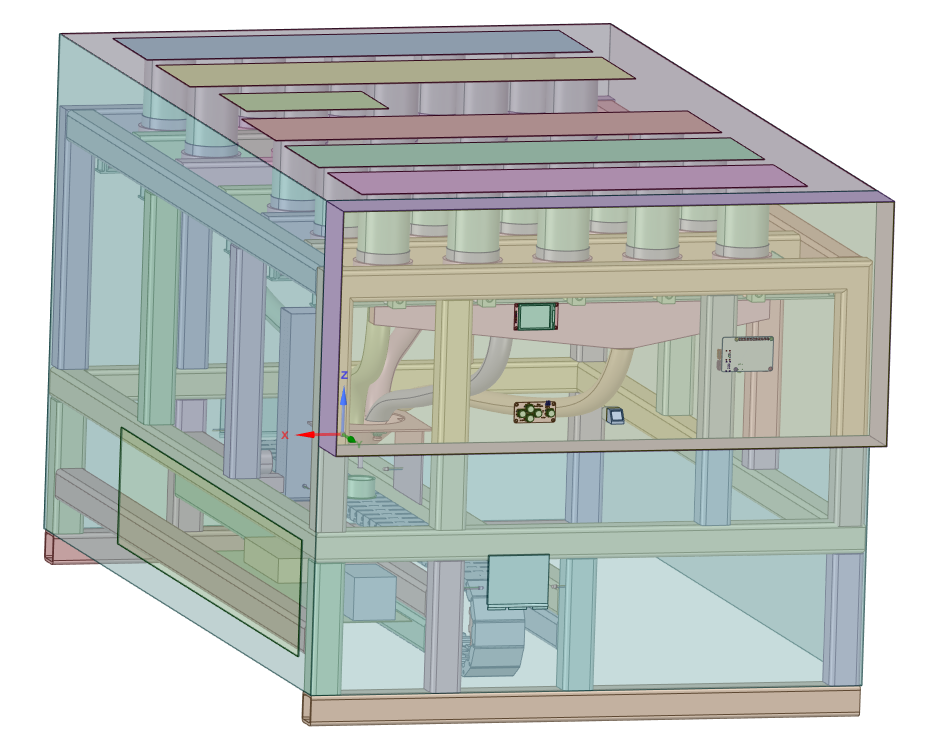
\includegraphics[width=.8\textwidth]{figuras/estrutura/Design/Vista completa com circuitaria.png}
%       \caption{Modelo em CAD da estrutura global}
%       \label{fig:Vista_completa}
%    \end{figure}

\section{Descrição dos componentes da Estrutura}

A seguir, estão descritos os componentes estruturais enumerados na Fig. \ref{fig:Descrição_Global}.

\begin{figure}[ht]
        \centering
        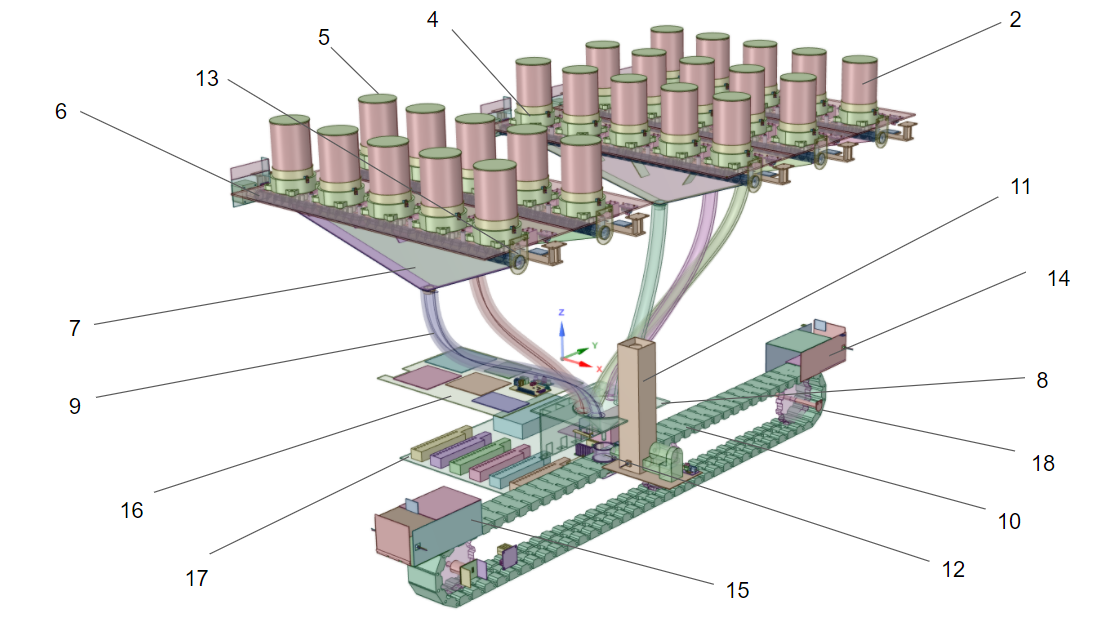
\includegraphics[width=1\textwidth]{figuras/estrutura/Design/descricao_estrutura.png}
        \caption{Descrição dos componentes da estrutura global}
        \label{fig:Descrição_Global}
    \end{figure}

    
%\begin{enumerate}
\subparagraph*{1.}
Estrutura principal: responsável pela proteção dos demais subsistemas, suportar esforços físicos e condições adversas de temperatura, pressão e umidade, além de impedir que o usuário entre em contato com os medicamentos sem autorização. A carcaça será constituída de:
% \begin{enumerate}

    \subparagraph*{a. } \label{retorno_tubos_perfilquadrado}
    Tubos de perfil quadrado:  Conjunto de tubos perfil quadrado, em formato de gaiola estrutural, a qual proporciona resistência estática e sustentação global das estruturas e de seus sistemas, assim como pontos de ancoragem e referência no projeto. Todos os comprimentos, localização e dimensão do perfil utilizado são apresentadas em seu desenho técnico na Fig. \ref{fig:estruturatubular}.
   \begin{itemize}
   \item[]
   \begin{itemize}
      \item Material: Aço carbono SAE 1020;
   \end{itemize}
   \end{itemize}
     
% \begin{enumerate}
    \subparagraph*{b. }  \label{retorno_chapas} 
    Chapas da Carcaça: Estrutura composta de chapas de alumínio, que envelopam a estrutura tubular, inibindo a entrada de agentes externos indesejáveis e auxiliando na resistência da estrutura, além de ancorar as dobradiças e componentes eletrônicos. As dimensões dessa estrutura estão apresentadas em seu desenho técnico na Fig. \ref{fig:chapasexterior}.
   \begin{itemize}
   \item[]
   \begin{itemize}
       \item Material das Chapas: Alumínio;
   \end{itemize}
   \end{itemize}
    
     
    \subparagraph*{c.} \label{Retorno_Mancal_de_suporte} 
    Mancais de suporte dos fusos: Os mancais serão utilizados para ancorar os rolamentos dos fusos, na medida que é necessário o uso de rolamentos para apoio e liberdade de rotação dos fusos. Para tanto, um rolamento rígido de esferas é ideal, na medida que a rotação do fuso é de baixa intensidade e a carga de apoio não é muito elevada. O rolamento escolhido foi o SKF W 61705, por apresentar dimensões satisfatórias para o projeto.   Suas dimensões são apresentadas em seus desenhos técnicso nas Fig. \ref{fig:Mancal_Fuso} e Fig. \ref{fig:rolamento_fuso}.
    
   \begin{itemize}
   \item[]
   \begin{itemize}
       \item  Material: Aço carbono SAE 1020;
       \item  Diâmetro interno do rolamento: 25 mm;
       \item  Diâmetro externo do rolamento: 32 mm;
       \item  Largura do rolamento: 4 mm;
       \item  Tipo de rolamento: SKF W 61705;
   \end{itemize}
   \end{itemize}
     
     
    
   \subparagraph*{d.} \label{retorno_suporte_atuador}  
   Estrutura para suporte do atuador linear do recipiente dos copos,composta de chapas de aço carbono SAE 1020, ancoradas na estrutura tubular para fomentar suporte. 
    Suas dimensões estão explicitadas neste desenho técnico na Fig. \ref{fig:repositorio}.
    
   \begin{itemize}
   \item[]
   \begin{itemize}
       \item Material: Aço Carbono SAE 1020;
   \end{itemize}
   \end{itemize}

    
     
    \subparagraph*{e.} \label{retorno_suporte_esteira}
    Engrenagens da esteira: Utilizadas para suportar e atribuir a dinamicidade de locomoção da esteira.  As dimensões das engrenagens são comerciais pelo próprio fabricante da esteira, e estão apresentadas no desenho técnico na Fig. \ref{fig:engrenagem_esteira}.

    \begin{itemize}
   \item[]
   \begin{itemize}
       \item Material: \textit{Nylon} 6.6;
   \end{itemize}
   \end{itemize}
     
    
    
    \subparagraph*{f.} \label{retorno_suporte_motordepasso}
    Estrutura de suporte para os motores de passo: Estrutura em formato de chapa, que serve de ancoragem dos motores de passo na estrutura, assim como os \textit{Drivers} dos motores. Suas dimensões estão especificadas no desenho técnico na Fig. \ref{fig:supp_motordepasso}.
    
    \begin{itemize}
   \item[]
   \begin{itemize}
       \item Material: Aço carbono SAE 1020;
   \end{itemize}
   \end{itemize}
     
    
    
    \subparagraph*{g.} \label{Retorno_suporte_motorDC}
    Estrutura de suporte para o motor DC: Estrutura em formato de chapa, utilizada para ancoragem do motor DC no plano paralelo às engrenagens da esteira.  As dimensões desse suporte são apresentadas em seu desenho técnico na Fig. \ref{fig:supp_motordc}.
    
    \begin{itemize}
   \item[]
   \begin{itemize}
       \item Material: Aço carbono SAE 1020;
   \end{itemize}
   \end{itemize}
     
% \end{enumerate}


\subparagraph*{2.}
Contêiner de medicamentos: Estrutura responsável pelo abrigo e preservação dos remédios inseridos na máquina. A especificação de cada componente é apresentada abaixo, e os desenhos técnicos de cada um estão apresentados no Apêndice E.
%\begin{enumerate}

    \subparagraph*{a.} \label{retorno_rampaseletora}
    Rampa seletora: Estrutura em formato circular com centro coincidente com o do contêiner, com um domo em formato de calota esférica no topo para que os remédios sejam direcionados às extremidades do contêiner. A rampa tem formato de cunha e é solidária ao domo. Com o movimento rotativo transmitido da engrenagem por meio de um eixo cilíndrico de extremidade hexagonal que se liga à porção inferior do domo, a estrutura de cunha com função de rampa rotaciona e empurra o comprimido para a plataforma de seleção.
    Seu desenho técnico está apresentado na Fig. \ref{fig:rampaseletora}.
    
    \begin{itemize}
   \item[]
   \begin{itemize}
       \item Material: Polipropileno Homopolímero;
   \end{itemize}
   \end{itemize}
     
    
    \subparagraph*{b.} \label{retorno_platosuperior}
    Plataforma de seleção: Peça cilíndrica posicionada abaixo da rampa seletora e fixada ao compartimento inferior por meio de parafusos. Na sua extremidade está localizado o furo retangular responsável pela seleção dos remédios do contêiner para transporte, as extremidades do furo são chanfradas e atuam como facilitadores para a descida dos remédios. No seu centro há um furo com um rolamento inserido e pelo qual passa a porção cilíndrica do eixo que movimenta a rampa seletora. A plataforma de seleção não apresenta movimento rotativo. 
    O rolamento do centro é um rolamento de rolos de agulhas com anéis usinados e um anel interno. Optou-se pelo uso de um rolamento porque as superfícies da plataforma e do eixo estariam sempre em contato e seu desgaste poderia liberar partículas dentro do contêiner, da mesma maneira, o uso de lubrificantes poderia contaminar os medicamentos. Os rolos de agulhas foram escolhidos por sua montagem compacta e considerando que este rolamento não servirá de apoio, portanto o único fator limitante é a rotação à qual ele será submetido. Um rolamento aplicável é o modelo NKI 20/16 com diâmetro (d) interno de 20 mm, espessura (B) de 16 mm e diâmetro externo (D) de 32 mm.
    As dimensões dessa estrutura são explicitadas em seu desenho técnico na Fig. \ref{fig:platosuperior}.
    
    \begin{itemize}
   \item[]
   \begin{itemize}
       \item  Material: Polipropileno Homopolímero;
   \end{itemize}
   \end{itemize}
   
    
    \subparagraph*{c.} \label{retorno_engrenagem_fundo}
    Engrenagem com eixo: Engrenagem helicoidal fabricada em peça única com um eixo escalonado em uma porção cilíndrica e uma extremidade com formato de prisma hexagonal que se encaixa à porção inferior do domo da rampa seletora. Na sua parte inferior, há um furo para o seu suporte.
    A porção cilíndrica tem diâmetro maior que a porção hexagonal, desta maneira, ela é inserida pelo fundo da montagem, através da base do compartimento inferior e da plataforma de seleção (cujo rolamento permite que a plataforma permaneça estática enquanto a rampa seletora se movimenta) e encaixada à rampa seletora. O movimento radial da engrenagem provém de um fuso, cujo eixo é perpendicular ao eixo da engrenagem, instalado solidário a um motor de passo. O desenho técnico da engrenagem se apresenta na Fig. \ref{fig:engrenagem_fundo}.
    
    
    Além da engrenagem, seu conjunto possui ainda uma arruela e um rolamento interno, explicitados em seus desenhos técnicos: a arruela de proteção está na Fig. \ref{fig:arruela} e o rolamento interno na Fig. \ref{fig:rolamento_engrenagem}.
    
    \begin{itemize}
   \item[]
  \begin{itemize}
%        \item Módulo da Engrenagem: 2 mm.
%        \item Número de dentes: 21.
%        \item Ângulo de pressão: 20$^{\circ}$.
%        \item Diâmetro do furo da engrenagem: 10 mm.
%        \item Diâmetro da seção circular do eixo: 20 mm.
%        \item Comprimento da seção circular: 32 mm.
%        \item Lado da extremidade hexagonal: 8,66 mm.
%        \item Comprimento da extremidade hexagonal: 10 mm.
        \item Material: \textit{Nylon} 6.6;
   \end{itemize}
   \end{itemize}
   
    
    \subparagraph*{d.} \label{retorno_compartimentoinferior}
    Compartimento inferior: Compartimento que funciona de base para a montagem do contêiner. Nele é fixada a plataforma de seleção e a parede cilíndrica do contêiner. Sua porção inferior possui dois furos, um central pelo qual o eixo da engrenagem passa e um na extremidade radial para a seleção do medicamento armazenado. Ele apresenta um pequeno macho de rosca na sua lateral para que ele se encaixe com um pequeno giro à base que sustenta cada fileira de contêineres, de forma semelhante ao que ocorre com o copo de um liquidificador. As dimensões desse componente são apresentadas em seu desenho técnico na Fig. \ref{fig:compartimentoinferior}.
    
    \begin{itemize}
   \item[]
   \begin{itemize}
       \item Material: Polipropileno Homopolímero;
   \end{itemize}
   \end{itemize}
     

    \subparagraph*{e.} \label{retorno_suporte_engrenagem}
    Suporte da Engrenagem: Pequena chapa retangular com extremidades arredondadas. Em seu centro há um pino que recebe uma arruela e se encaixa à porção inferior da engrenagem. Em cada uma das extremidades projeta-se um tubo pelos quais são passados os parafusos de fixação do suporte, estes se prendem à mesa de apoio utilizando uma porca. As dimensões deste suporte são apresentadas no desenho técnico da Fig. \ref{fig:supp_engrenagem}.
    
    \begin{itemize}
   \item[]
   \begin{itemize}
       \item Material: Polipropileno Homopolímero;
   \end{itemize}
   \end{itemize}
     
   
    \subparagraph*{f.}\label{retorno_cilindro}
    Parede cilíndrica: Chapa de pequena espessura feita de aço inoxidável curvada e soldada ou conformada mecanicamente até formar um cilindro. Encaixa-se no compartimento inferior em uma porção vazada da sua região superior. Em cima dessa estrutura, é encaixada uma tampa para garantir o melhor isolamento possível do contêiner. As dimensões do cilindro são apresentadas no desenho técnico da Fig. \ref{fig:cilindro}.
    \begin{itemize}
   \item[]
   \begin{itemize}
       \item  Material da parede cilíndrica: Aço inoxidável SAE 304;
   \end{itemize}
   \end{itemize}
     
    
    \subparagraph*{3.} \label{retorno_comporta}
    Comporta do solenoide: Pequena chapa de material polimérico e formato semelhante a um trapézio com as bases arredondadas e uma estrutura triangular de suporte. Posiciona-se na extremidade inferior do contêiner, abaixo do compartimento inferior e encontra-se normalmente fechada. Está fixada por parafuso a um solenoide com retorno por mola e recua quando necessária a liberação de um medicamento. O solenoide é aparafusado à mesa de apoio. As dimensões desse componente estão explicitadas em seu desenho técnico da Fig. \ref{fig:comporta}.
    
     \begin{itemize}
   \item[]
   \begin{itemize}
       \item  Material: Polipropileno Homopolímero;
   \end{itemize}
   \end{itemize}
    
    
    \subparagraph*{4.}\label{retorno_conector}
    Base conectora do contêiner: Unida mecanicamente por quatro parafusos à mesa de apoio, possui um furo com rosca fêmea para o encaixe do compartimento inferior do contêiner, impedindo tanto seu movimento axial quanto radial. As dimensões dessa estrutura são apresentadas no desenho técnico da  Fig. \ref{fig:conector}.
    
    \begin{itemize}
   \item[]
   \begin{itemize}
       \item  Material: Polipropileno Homopolímero;
   \end{itemize}
   \end{itemize}
         
     
     \subparagraph*{5.}\label{retorno_tampa}
     Tampa de vedação: Componente cujo objetivo é de vedação da parte superior do cilindro dos contêineres, evitando a entrada de ar e outros agentes externos em contato direto com os comprimidos. As dimensões desse componente estão apresentados em seu desenho técnico  da Fig. \ref{fig:tampa}.
     
     \begin{itemize}
   \item[]
   \begin{itemize}
       \item  Material: Polipropileno Homopolímero;
   \end{itemize}
   \end{itemize}
      
    
%\end{enumerate}

\subparagraph*{6.}\label{retorno_base_subgrupo}
Mesa de apoio: Local responsável por estabelecer a sustentação do suporte e promover local de encaixe para os 25 contêineres, assim como para fixação dos solenoides e de seus \textit{Drivers}. As dimensões dessa estrutura estão apresentadas em seu desenho técnico da Fig. \ref{fig:base_subgrupo}.

\begin{itemize}
   \item[]
   \begin{itemize}
       \item  Material: Aço carbono SAE 1020;
   \end{itemize}
   \end{itemize}
 

\subparagraph*{7.}\label{retorno_zonadetransição}
Zona de transição: Região composta por estrutura tubular que se deriva em canaletas, uma por cada subgrupo de 5 contêineres, onde o medicamento será direcionado para a mangueira de silicone, possibilitando seu movimento até o copo especificado. Os desenhos técnicos desses componentes, que compreendem as canaletas, canal de guia e suporte do canal de guia, são apresentados abaixo:

\begin{itemize}
   \item[]
   \begin{itemize}
       \item Canaleta do subgrupo 1 - Fig. \ref{fig:canaletaS1}.
       \item Canaleta do subgrupo 2 - Fig. \ref{fig:canaletaS2}.
       \item Canaleta do subgrupo 3 - Fig. \ref{fig:canaletaS3}.
       \item Canaleta do subgrupo 4 - Fig. \ref{fig:canaletaS4}.
       \item Canaleta do subgrupo 5 - Fig. \ref{fig:canaletaS5}.
       \item Canal de guia - Fig. \ref{fig:canalguia}.
       \item Suporte do canal de guia - Fig. \ref{fig:supp_canal}.
       \item Material dos componentes: Polipropileno Homopolímero;
   \end{itemize}
   \end{itemize}

 
 \subparagraph*{8.}\label{retorno_funil}
 Funil de saída: Objeto afunilado que será o ponto de término dos comprimidos após a saída das mangueiras de silicone, depositando-os dentro do copo, na posição inicial. Suas dimensões são apresentadas em seu desenho técnico da Fig. \ref{fig:funil}.
 
 \begin{itemize}
   \item[]
   \begin{itemize}
       \item  Material do Funil: Alumínio;
   \end{itemize}
   \end{itemize}
  
  
 \subparagraph*{9.}\label{retorno_mangueira}
 Mangueiras de Silicone: Mangueiras que funcionam como dutos de orientação dos medicamentos até seu destino final, o funil de despejo nos copos. As dimensões dessas estruturas são explicitadas em seus desenhos técnicos:
 
 
 \begin{itemize}
    \item[]
    \begin{itemize}
    \item  Mangueira do Subgrupo 1 - Fig. \ref{fig:M_S1};
    \item  Mangueira do Subgrupo 2 - Fig. \ref{fig:M_S2};
    \item  Mangueira do Subgrupo 3 - Fig. \ref{fig:M_S3};
    \item  Mangueira do Subgrupo 4 - Fig. \ref{fig:M_S4};
    \item  Mangueira do Subgrupo 5 - Fig. \ref{fig:M_S5};
    \item Material das mangueiras: Silicone;
     \end{itemize}
 \end{itemize}
 

\subparagraph*{10.}\label{retorno_esteira}
Esteira: Objeto utilizado para fazer o transporte do recipiente com os medicamentos selecionados para o compartimento frontal ou traseiro. Essa estrutura é formada por pequenas plataformas de acetal, interligadas por pinos de aço inoxidável, com suas dimensões especificadas em seu desenho técnico, disposto na Fig.\ref{fig:esteira}


\begin{itemize}
    \item[]
    \begin{itemize}
    \item  Material dos módulos da esteira: Acetal;
    \item  Material dos pinos: Aço Inox AISI 304;
    \item  Peso linear da plataforma com pinos: Aproximadamente 1 kg/m;
    \end{itemize}
\end{itemize}   

\subparagraph*{11.}\label{retorno_reservatorio}
Reservatório de copos: Local responsável por armazenar os copos responsáveis para deposição dos medicamentos. Essa estrutura está localizada em um plano adjacente a esteira, e há uma limitação por cantoneiras circulares internamente, para que não haja movimento dos copos dentro da estrutura. As dimensões dessa estrutura são especificadas em seu desenho técnico na Fig. \ref{fig:repositorio}.

\begin{itemize}
   \item[]
   \begin{itemize}
       \item  Material: Aço carbono SAE 1020;
   \end{itemize}
   \end{itemize}
  

\subparagraph*{12.} \label{retorno_copo}
Copo dos medicamentos: Recipiente responsável por resguardar os medicamentos selecionados pela Central de Comando, que passaram pela Zona de Transição e são depositados sobre o mesmo, na posição inicial de despejo. Suas dimensões são explicitadas no desenho técnico, compreendido na Fig. \ref{fig:copo}.

\begin{itemize}
   \item[]
   \begin{itemize}
       \item Material: Polipropileno Homopolímero;
   \end{itemize}
   \end{itemize}


\subparagraph*{13.}\label{retorno_fuso}
Fuso de acoplamento: Estrutura em formato de parafuso sem-fim com coincidência central no eixo dos motores de passo de cada subgrupo, e suportado por meio de um rolamento rígido de esferas, dentro de um mancal de suporte, oposto ao motor de passo. As dimensões do fuso são especificadas no desenho técnico da Fig. \ref{fig:fuso}.

\begin{itemize}
   \item[]
   \begin{itemize}
       \item Material: \textit{Nylon} 6.6;
   \end{itemize}
   \end{itemize}
 

\subparagraph*{14.} \label{retorno_porta}
Compartimento Anterior: Área onde será efetuada a retirada dos recipientes com medicação extra (com falhas), ou em falta, pelo usuário. Ela é composta tanto pela Zona de retorno quanto pela porta de saída de retorno. As dimensões desses elementos são apresentadas em seus desenhos técnicos nas Fig. \ref{fig:porta_saida} e Fig. \ref{fig:zona_retorno}.

 \begin{itemize}
   \item[]
   \begin{itemize}
       \item Material: Aço carbono SAE 1020;
   \end{itemize}
   \end{itemize}

\subparagraph*{15.}
Compartimento frontal: Área onde será efetuada a retirada dos recipientes com medicação correta pelo usuário. Essa região é composta pela área de espera e pela porta de saída correta. As dimensões desses elementos são apresentadas nas Fig. \ref{fig:porta_saida} e Fig. \ref{fig:area_espera}.

 \begin{itemize}
   \item[]
   \begin{itemize}
       \item Material: Aço carbono SAE 1020;
   \end{itemize}
   \end{itemize}
   
 \subparagraph*{16.} \label{retorno_Centro_PCBs}
 Centro de comunicação das PCBs: Chapa utilizada para ancoragem e organização das PCBs, assim como da \textit{Raspberry}. Seu desenho técnico, possuindo a fixação de cada componente, está explicitado na Fig. \ref{fig:Centro_PCBs}.

\begin{itemize}
   \item[]
   \begin{itemize}
       \item Material: Aço carbono SAE 1020;
   \end{itemize}
   \end{itemize} 

 \subparagraph*{17.} \label{retorno_suporte_energia}
 Suporte dos componentes energéticos: Chapa utilizada para ancoragem e disposição dos componentes energéticos, compreendendo bateria, fonte chaveada, PCBs e \textit{bornes}. O desenho técnico dessa estrutura se encontra na Fig. \ref{fig:suporte_energia}.
 
  \begin{itemize}
   \item[]
   \begin{itemize}
       \item Material: Aço carbono SAE 1020;
   \end{itemize}
   \end{itemize} 
  
 \subparagraph*{18.} \label{retorno_Eixos_Esteira}
 Eixos de suporte da esteira: Eixos solidários às engrenagens de sustentação da esteira, ancorados por mancais nos tubos paralelos à esteira. O desenho técnico dessa estrutura está apresentado na Fig. \ref{fig:Eixos_Esteira}.
 
 \begin{itemize}
   \item[]
   \begin{itemize}
       \item Material: \textit{Nylon} 6.6;
   \end{itemize}
   \end{itemize} 
  
  \subparagraph*{19.} \label{retorno_suporte_interruptor}
  Suporte dos interruptores: Estrutura composta por chapas que funcionam como \textit{housing} dos interruptores na estrutura. O desenho técnico é disposto na Fig. \ref{fig:suporte_interruptor}
  
  \begin{itemize}
   \item[]
   \begin{itemize}
       \item Material: Aço carbono SAE 1020;
   \end{itemize}
   \end{itemize} 
   
%\end{enumerate}

\section{Desenhos técnicos}
Os desenhos técnicos da estrutura e seus componentes estão disponíveis no Apêndice \ref{cad_preliminar}.

\section{Dinâmica de operação}
\label{sec:dinamica_operacao}

Após identificados os componentes do sistema, temos a exemplificação de seu funcionamento, feita preliminarmente via o fluxograma da Fig. \ref{fig:FEst}.

\begin{figure}[ht] %tem necessidade de alterar o tamanho dessa imagem?
        \centering
        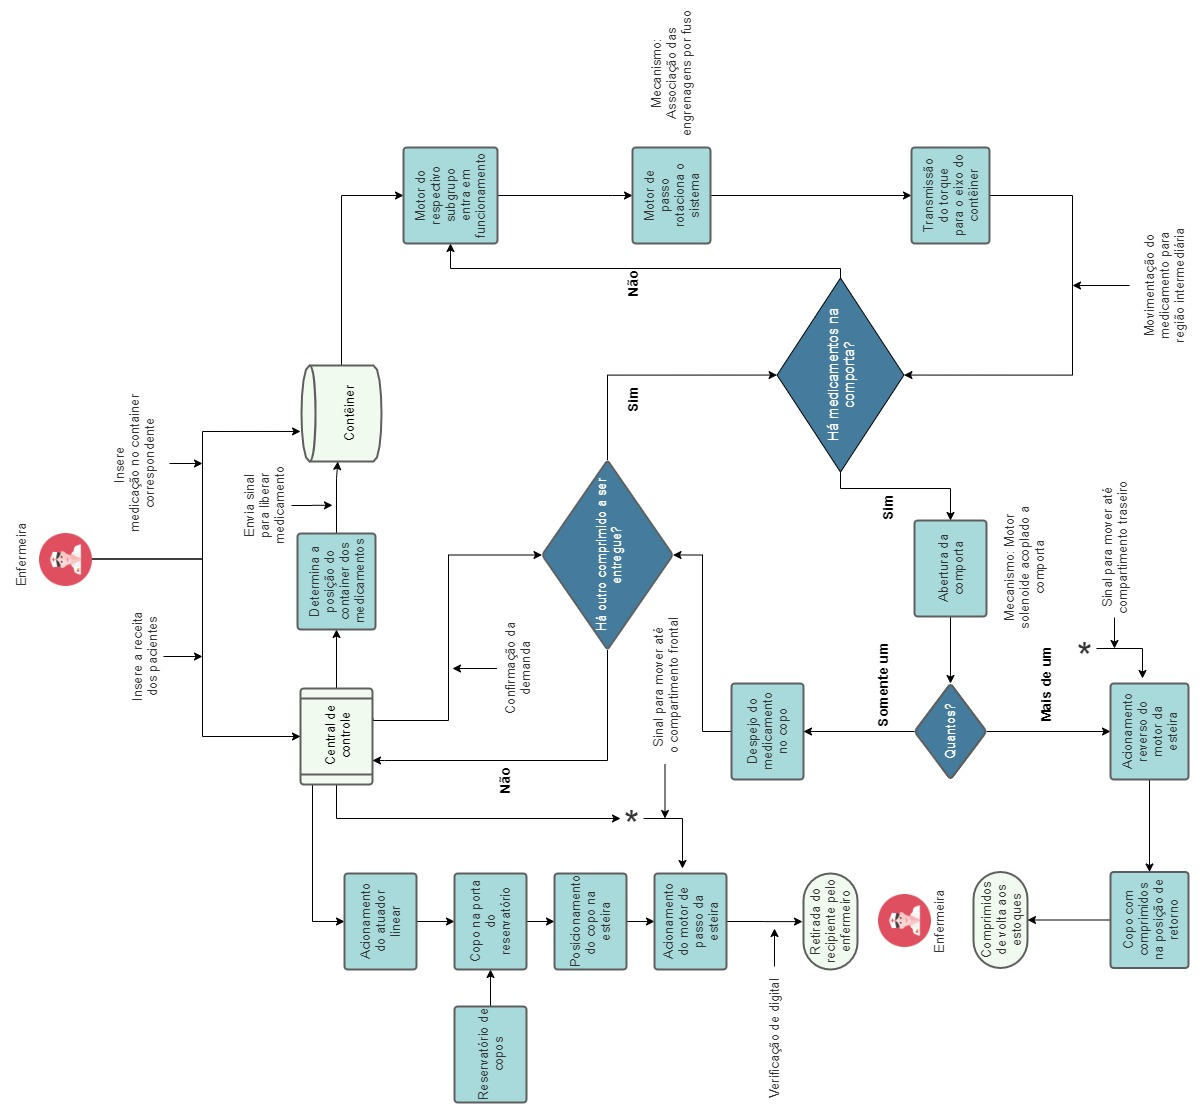
\includegraphics[width=1\textwidth, angle = -90]{figuras/estrutura/FEstrV35.jpg}
        \caption{Fluxograma de operação do Sistema Mecânico}
        \label{fig:FEst}
    \end{figure}

\paragraph*{O processo é iniciado:}

\begin{enumerate}
    \item[1.] Inserção de dados feita pelo enfermeiro do usuário e a respectiva entrada dos medicamentos no Contêiner.
    \item[2.] Determinação da posição dos contêineres dos medicamentos pela central de controle.
    \item[3.] Envio do sinal para liberar a medicação por demanda.
    \end{enumerate} 
   
% O conjunto abaixo entraria em ação após execução da etapa 3.
\paragraph*{O conjunto abaixo entraria em ação após execução da etapa 3:}

\begin{enumerate}
    \item [4.] Acionamento do micro atuador linear por demanda da central de controle.
    \item [5.] Posicionamento do copo no local de deposição dos medicamentos o e o recipiente adjacente (próximo copo) assume a posição inicial após o retorno do atuador linear para a posição de repouso.
    \item [6.] Pausa até a verificação de funcionamento dos motores de passo ser concluída.
\end{enumerate}
    
    % Enquanto a movimentação do copo pela esteira se conclui, a ação do sistema de seleção tem início:
\paragraph*{Enquanto a movimentação do copo pela esteira se conclui, a ação do sistema de seleção tem início:}

\begin{enumerate}
    \item[7.] Verificação da presença de medicamentos na região intermediária do sistema (anterior à comporta).
    \item[8.] Abertura da comporta do contêiner por motor solenoide.
    \item[9.] Verificação da quantidade de comprimidos despejados pelo sistema no recipiente do usuário (copo).
\end{enumerate}
   
    % Caso não seja detectada a presença do medicamento na região intermediária (parte  anterior à comporta), a sequência ocorre:
\paragraph*{Caso não seja detectada a presença do medicamento na região intermediária (parte  anterior à comporta), a sequência ocorre:}

\begin{enumerate}
    \item[10.] Início da operação do motor do subgrupo do contêiner selecionado.
    \item[11.] Motor de passo rotaciona o fuso.
    \item[12.] Transmissão do torque para os eixos dos contêineres por meio de engrenagens helicoidais.
    \item[13.] Posicionamento do remédio na plataforma de seleção do contêiner.
    \item[14.] Abertura da comporta do contêiner por motor solenoide.
    \item[15.] Checagem de sensores da queda dos medicamentos para repetição ou fim do ciclo de rotação.
    \item[16.] Verificação da quantidade de comprimidos despejados pelo sistema no recipiente do usuário (copo).
    \item[17.] Repetição do ciclo a partir da etapa 7 até que todos os comprimidos selecionados sejam entregues.
\end{enumerate}


    % Durante o processo de escolha dos medicamentos do paciente, a verificação irá traduzir na atuação da esteira como segue:
\paragraph*{Durante o processo de escolha dos medicamentos do paciente, a verificação irá traduzir na atuação da esteira como segue:}

\begin{enumerate}
    \item[18a.] A medicação é verificada e não há erros detectados pelos sensores.
    \item[19a.] Acionamento do motor de passo da esteira no sentido usual.
    \item[20a.] Operação da esteira até local de retirada do enfermeiro. 
    \item[21a.] Verificação de digital e abertura do compartimento frontal.
\end{enumerate}
   
\paragraph*{Caso seja identificada alguma falha:}

\begin{enumerate}
    \item[18b.] A medicação é verificada e erros são encontrados pelos sensores.
    \item[19b.] Acionamento reverso do motor da esteira.
    \item[20b.] Operação da esteira até o compartimento traseiro.
    \item[21b.] Despejo do copo no compartimento traseiro.
    \item[22b.] Medicação extra preparada para remoção pelo enfermeiro.
\end{enumerate}

\section{Escolha de Materiais}
No desenvolvimento de tecnologias médicas, a escolha dos materiais assume um papel de suma importância, pois nestes casos, os materiais deverão atender não somente requisitos de engenharia estrutural, mas também aos protocolos de segurança da saúde \cite{Steel_Group}.

Com o aumento das restrições de projeto, há uma diminuição da quantidade de materiais disponíveis para atender a solução, dessa forma, a escolha se torna mais limitada e responsável. Os materiais apresentados a seguir, tiveram sua escolha baseada em três segmentos gerais: segurança sanitária; propriedades de engenharia e custos.

\subparagraph*{$\bullet$ Aço Inoxidável 304} \hfill

O tipo de aço inox escolhido pertence a família dos austeníticos, o que significa que ele é composto basicamente por: ferro; cromo e níquel. Temos assim, a garantia de uma alta resistência à oxidação, corrosão, boa conformabilidade e boa soldabilidade \cite{Askeland_Wright_2019}. Além das vantagens já apresentadas, o aço Inox 304 possui características essenciais para o setor da saúde:
\begin{itemize}
    \item []

    \begin{itemize}
        \item Superfície não porosa, o que proporciona uma diminuição do risco de contaminação por bactérias e vírus.
        \item Resistente a produtos químicos.
        \item Fácil higienização.
        \item Material não magnético. 
        \item Resistente ao Calor.
        \item Reciclável.
    \end{itemize}
\end{itemize}
    

\begin{table}[H]
    \centering
    \caption{Propriedades do Aço Inox 304 \cite{Askeland_Wright_2019}.}
    \label{fig:PropAI}
    \begin{adjustbox}{max width = \textwidth}
        \begin{tabular}{|C{1.5cm}|C{1.5cm}|C{1.5cm}|C{1.5cm}|C{3cm}|C{3cm}|C{2.8cm}|C{3cm}|}
            \hline
            \rowcolor[HTML]{A8DADC}
            \textbf{Aço} & \textbf{\%C} & \textbf{\%Cr} & \textbf{\%Ni} & \textbf{Limite de Resistencia [MPa]} & \textbf{Limite de Escoamento [MPa]} & \textbf{Alongamento [\%]} & \textbf{Massa Específica [kg/m$^3$]}  \\ \hline
            
              Inox 304 & 0,08 & 0,19 & 0,10  & 517 & 207 & 30 & 8030              \\ \hline
            
        \end{tabular}
    \end{adjustbox}
\end{table}

\subparagraph*{$\bullet$ Aço-carbono 1020}\hfill

O material em questão foi escolhido por apresentar características técnicas e orçamentárias que contribuem para o sucesso do projeto. Segundo \cite{Aco_1020_ensaio}, a quantidade de cementita apresentada na metalografia do aço 1020 proporciona ótima resistência à traç{\~a}o e propriedades mecânicas para as mais diversas aplicações industriais. Serão utilizados tanto aço de classificação SAE como da classificação AISI, não por requisitos estruturais, mas pela disponibilidade no mercado e pelo escopo de custos do projeto. Seguem os fatores responsáveis pela escolha do aço-carbono 1020:

\begin{itemize}
    \item []
    \begin{itemize}
        \item Boa conformabilidade.
        \item Boa soldabilidade.
        \item Custo-benefício.
    \end{itemize}
\end{itemize}

\begin{table}[H]
    \centering
    \caption{Propriedades do Aço 1020 \cite{Askeland_Wright_2019}.}
    \label{tab:PropA1020}
    \begin{adjustbox}{max width = \textwidth}
        \begin{tabular}{|C{2cm}|C{2cm}|C{2cm}|C{3cm}|C{3cm}|C{3cm}|C{2.8cm}|C{2cm}|C{3cm}|}
            \hline
            \rowcolor[HTML]{A8DADC}
            \textbf{Aço } & \textbf{\%C} & \textbf{\%Mn} & \textbf{Limite de Resistência [MPa]} & \textbf{Limite de Escoamento [MPa]} & \textbf{Alongamento [\%]} &
            \textbf{Massa Específica [kg/m$^3$]} \\ \hline
            
              Carbono 1020 & 0,18-0,23 & 0,30-0,60 & 450  & 330 & 36 & 7850
             \\ \hline
            
        \end{tabular}
    \end{adjustbox}
\end{table}

%\subparagraph*{$\bullet$ Polipropileno (PP)}\hfill


\subparagraph*{$\bullet$ Polipropileno (PP)}\hfill 

 A transmissão dos gases, vapores, ou líquidos através dos materiais de embalagem primária, conhecidos como blisters, pode ter um efeito adverso sobre o prazo de validade do medicamento. A permeabilidade do vapor de água ou do oxigênio através do material de embalagem pode constituir um problema se a forma farmacêutica for sensível à hidrólise ou oxidação \cite{embalagem}. Ao retirar o remédio da fonte de proteção primária, deve-se atentar aos efeitos físico-químicos consequentes da exposição do mesmo a condições adversas. 

Com o intuito de promover uma armazenagem segura da dose medicamentosa, o aspecto de permeabilidade e absorção do material, os quais quantificam o movimento de difusão de pequenas moléculas externas (O$_2$, H$_2$O, CO$_2$, CH$_4$) no material, representam um papel fundamental na escolha do polímero \cite{materiais}.  

Para tanto, pelas características limitantes do presente projeto, foi se escolhido o polipropileno devido aos critérios de: 

\begin{itemize} 

    \item[ ] 

    \begin{itemize} 

        \item Baixo custo. 

        \item Reciclável. 

        \item Comportamento mecânico.  

        \item Comportamento plástico. 

        \item Comportamento dúctil. 

        \item Atoxidade 

        \item Baixa absorção de umidade (baixa permeabilidade). 

        \item Resistência química. 

        \item Resinas com baixo potencial de contaminação 
    \end{itemize} 

\end{itemize} 

 

 

Se tratando de um material que será utilizado como componente estrutural da solução, o estudo do comportamento mecânico e suas propriedades devem ser analisado de forma criteriosa. As principais propriedades do polipropileno são apresentadas na Tab. \ref{tab:PropPP}.  

  

\begin{table}[ht] 

    \centering 

    \caption{Propriedades do Polipropileno (PP) \cite{materiais}.} 

    \label{tab:PropPP} 

    \begin{adjustbox}{max width = \textwidth} 

        \begin{tabular}{|C{3cm}|C{3cm}|C{2.8cm}|C{3cm}|C{2.5cm}|} 

            \hline 

            \rowcolor[HTML]{A8DADC} 

            \textbf{Polímero} & \textbf{Resistência a tração [MPa]} & \textbf{Alongamento [$\%$]} & \textbf{Módulo  de Elasticidade [GPa]} & \textbf{Massa Específica [kg/m$^3$]} \\ \hline 

             

              Polipropileno (PP) & 25-40 & 150-600 & 0,90-1,60  & 900 

             \\ \hline 

        \end{tabular} 

    \end{adjustbox} 

\end{table} 
Disponível comercialmente em diversas formas, o PP ideal para aplicação neste projeto é na forma de homopolímero (PP-HOMO), pois além de todas as características desejadas, também permite limpeza com detergentes e possibilidade de esterilização a vapor. Uma alternativa é a utilização de copolímeros de polipropileno de aplicação médica como o \textit{Purell}. \cite{HMC_poly}.

%Disponível comercialmente em diversas formas, o PP ideal para aplicação neste projeto é na forma de homopolímero (PP-HOMO), pois além de todas as características desejadas, também permite limpeza com detergentes e possibilidade de esterilização a vapor. Uma alternativa é a utilização de copolímeros de polipropileno de aplicação médica como o \textit{Purell}. \cite{HMC_poly}. 
%O movimento de difusão de pequenas moléculas externas (O$_2$, H$_2$O, CO$_2$, CH$_4$) nos polímeros são fatores que influenciam na escolha  do material, pois características de permeabilidade e de absorção de um polímero estão relacionadas com o grau no qual as substâncias externas se difundem no material. A entrada de substâncias externas pode levar ao inchamento e/ou a reações químicas com o polímero, gerando à degradação das propriedades mecânicas e físicas do material \cite{materiais}. 

%O coeficiente de permeabilidade caracteriza a difusão dos polímeros para determinadas aplicações, e pelas características limitantes do presente projeto, as taxas de permeabilidade (Pm) devem ser baixas, fator que contribuiu para a escolha do presente polímero. Na Tab. \ref{tab:coef_permeabilidade}, pode-se observar os valores dos coeficientes de permeabilidade para os principais elementos químicos que podem estar presentes no meio externo e interno da solução a ser desenvolvida. 

%\begin{table}[H]
%    \centering
%    \caption{Coeficientes de Permeabilidade (Pm) a 25°C para o Oxigênio, Nitrogênio, Dióxido de Carbono e Vapor d’Água}
%   \label{tab:coef_permeabilidade}
%    \begin{adjustbox}{max width = \textwidth}
 %       \begin{tabular}{|C{3cm}|C{4.5cm}|C{4.5cm}|C{4.5cm}|C{4.5cm}|C{4.5cm}|}
 %%          \hline
%            \rowcolor[HTML]{A8DADC}
%            \textbf{Polímero} & 
%            
%            \textbf{O2 $10 \to13 \;\frac{(cm^3 \, CNTP)(cm)}{(cm^2\cdot s\cdot P)}$} & 
%            \textbf{N2 $10 \to13 \;\frac{(cm^3 \, CNTP)(cm)}{(cm^2\cdot s\cdot Pa)}$} & 
%            \textbf{CO2 $10 \to13 \;\frac{(cm^3 \, CNTP)(cm)}{(cm^2\cdot s\cdot Pa)}$} &
%            \textbf{H2O $10 \to13 \;\frac{(cm^3 \, CNTP)(cm)}{(cm^2\cdot s\cdot Pa)}$} 
%           \\ \hline
%            
%              Polipropileno (PP) & 1,2 & 0,22  & 5,4 & 38
%             \\ \hline
%        \end{tabular}
%    \end{adjustbox}
%\end{table}

%Se tratando de um material que será utilizado como componente estrutural da solução, o estudo do comportamento mecânico e suas propriedades devem ser analisado de forma criteriosa. As principais propriedades do polipropileno são apresentadas na Tab. \ref{tab:PropPP}. 

%\begin{table}[H]
%    \centering
%    \caption{Propriedades do Polipropileno (PP). \cite{materiais}.}
%    \begin{adjustbox}{max width = \textwidth}
%        \begin{tabular}{|C{3cm}|C{3cm}|C{2.8cm}|C{3cm}|C{2.5cm}|}
%            \hline
%            \rowcolor[HTML]{A8DADC}
%            \textbf{Polímero} & \textbf{Resistência a tração (MPa)} & \textbf{Alongamento ($\%$)} & \textbf{Módulo  de Elasticidade (GPa)} & \textbf{Massa Específica (kg/m$^3$)} \\ \hline
%            
%              Polipropileno (PP) & 25-40 & 150-600 & 0,90-1,60  & 900
%             \\ \hline
%        \end{tabular}
%    \end{adjustbox}
%\end{table}

%O presente polímero termoplástico foi escolhido depois de se assumir requisitos essenciais para o sucesso do projeto e buscar o material que mais se adequasse a essas exigências. Segundo \cite{PP_Recycle}, o polipropileno é muito utilizado na indústria farmacêutica para frascos de prescriç{\~a}o, recipientes de medicamentos, tanto ovais como cilíndricos e quadrados, e também para fechamento de recipientes. A seguir são listadas as características responsáveis pela escolha do polipropileno: 

%\begin{itemize}
%    \item[ ]
%    \begin{itemize}
%        \item Baixo custo.
%        \item Reciclável.
%        \item Comportamento mecânico. 
%        \item Comportamento plástico.
%        \item Comportamento dúctil.
%        \item Atoxidade
%        \item Baixa absorção de umidade.
%        \item Resistência química.
%        \item Resinas com baixo potencial de contaminação
%    \end{itemize}
%\end{itemize}

%Disponível comercialmente em diversas formas, o PP ideal para aplicação neste projeto é na forma de homopolímero (PP-HOMO), apresentando excelente resistência mecânica, química e térmica, permitindo, por exemplo, limpeza com detergentes e esterilização a vapor. Também é possível a utilização de copolímeros de polipropileno de aplicação médica como o \textit{Purell}. \cite{HMC_poly}.

\subparagraph*{$\bullet$ Nylon 6.6 (Poliamida PA 6,6)} \hfill

A escolha do \textit{Nylon} para o projeto se deu pela sua facilidade de manipulação e custo operacional. Segundo \cite{Imp3D_Polimeros}, o \textit{Nylon} é um plástico de baixo custo, forte, leve e flexível, que possui propriedades como estabilidade dimensional, boa resistência ao impacto sem entalhe e excelente resistência química. Ele é muito utilizado tanto para Impressão 3D de componentes, como para extrusão, injeção e até mesmo usinagem de peças.

\begin{table}[H]
    \centering
    \caption{Propriedades do \textit{Nylon} 6.6 (PA 6,6) \cite{mechanicalPolymers}.}
    \label{tab:PropPA6}
    \begin{adjustbox}{max width = \textwidth}
        \begin{tabular}{|C{2cm}|C{3cm}|C{3cm}|C{3cm}|C{2.5cm}|}
            \hline
            \rowcolor[HTML]{A8DADC}
            \textbf{Polímero} & \textbf{Resistência a tração [MPa]} & \textbf{Alongamento [$\%$] } & \textbf{Módulo de Elasticidade [GPa]} & \textbf{Massa Específica [kg/m$^3$]} \\ \hline
            
              \textit{Nylon} 6.6 & 80-84 & 60-300 & 1,80-3,30 & 1140
             \\ \hline
        \end{tabular}
    \end{adjustbox}
\end{table}

\subparagraph*{$\bullet$ Acrilonitrila Butadieno Estireno (ABS)}\hfill

O ABS é um copolímero utilizado na impressão 3D que traz um alto grau de detalhamento para as peças. Segundo \cite{Imp3D_Polimeros}, o ABS é superior ao PLA em relação à propriedades mecânicas, é durável, forte e é considerado leve. Suporta altas temperaturas e é um dos termoplásticos mais baratos no mercado de filamentos.

Ele foi utilizado para a cotação dos valores de impressão 3D de um protótipo do produto final, uma vez que suas condições de processamento em impressão mais são próximas do Polipropileno e \textit{Nylon} que outros materiais usuais como PLA e PETG.

\subparagraph*{$\bullet$ Silicone} \hfill

O silicone também possui papel fundamental neste projeto, pela sua alta maleabilidade de uso. Segundo \cite{Silicone_estudo}, o silicone é utilizado para resistir a altas temperaturas, resistência às intempéries, biocompatibilidade, além de alta estabilidade, baixa tensão superficial e falta de toxicidade, o que permite sua utilização com medicamentos.

\section{Processos de Fabricação} 
\label{section:fabricacao}

\subparagraph*{$\bullet$ Estrutura principal tubular} \hfill

O aço carbono SAE 1020 apresenta boa soldabilidade e faz com que a estrutura tubular possa ser fabricada por processos simples de corte, desbaste e soldagem MIG, que apresenta boa relação entre resistência, facilidade de execução, acabamento e custo, quando comparada aos processos de eletrodo revestido e TIG.

A base tem seus tubos cortados em ângulos de 45$^{\circ}$, unidos por solda, desbastada até que as faces fiquem homogêneas. Os tubos verticais recebem cortes em ângulos retos nas suas extremidades e unidos à base por soldagem em volta do seu perímetro. Os tubos horizontais da região central seriam unidos pelo seu perímetro às laterais dos tubos verticais. Os tubos do topo seriam unidos de forma análoga ao processo da base.

Ainda por soldagem, seriam unidas as abas de fixação dos demais componentes estruturais, eletrônicos e de acabamento externo. Após a inspeção do resultado, a estrutura tubular, e seus apêndices, passaria por um processo de lixamento, aplicação de fundo anti-corrosão e pintura.

\subparagraph*{$\bullet$ Mancais de suporte dos fusos} \hfill

Necessitam ter a espessura do rolamento que vai ser montado neles somada à espessura de um batente. Assim, é preciso realizar o corte de uma placa de espessura adequada, provavelmente a plasma, laser ou jato d'água. A placa cortada então teria seu centro usinado em um torno de bancada com as medidas corretas para a montagem por interferência do rolamento. Por fim, seria realizada a furação para a fixação na estrutura principal.

\subparagraph*{$\bullet$ Suporte do atuador linear do recipiente de copos} \hfill

Produzido em chapas de aço carbono SAE 1020 cortadas e soldadas por solda MIG na geometria apresentada com furações para a fixação do atuador.

\subparagraph*{$\bullet$ Suporte da esteira} \hfill

Usinagem de um tarugo de aço com chaveta para encaixe na engrenagem da esteira fabricada comercialmente.

\subparagraph*{$\bullet$ Suporte dos motores de passo} \hfill

Chapa de aço carbono SAE 1020 cortada e furada para permitir a fixação por parafusos do motor de passo. Esse suporte é uma aba soldada por solda MIG na estrutura principal.

\subparagraph*{$\bullet$ Suporte do motor DC da esteira} \hfill

Produzido em chapas de aço carbono SAE 1020 cortadas e soldadas em solda MIG na geometria apresentada com furações para a fixação do atuador.

\subparagraph*{$\bullet$ Componentes poliméricos do contêiner} \hfill

Os seguintes componentes seriam produzidos por impressão 3D com filamento de Polipropileno Homopolímero(PP-HOMO) para a manufatura do protótipo, uma vez que entram em contato direto com os medicamentos. Para uma produção em escala, o ideal é que sejam produzidos por injeção em molde fechado.

\begin{itemize}
    \item Rampa seletora;
    \item Plataforma de seleção;
    \item Compartimento inferior;
    \item Comporta do solenoide;
    \item Tampa;
    \item Base para fixação do contêiner.
\end{itemize}

\subparagraph*{$\bullet$ Parede cilíndrica do contêiner} \hfill 

Encaixada no compartimento inferior do contêiner, é produzida em uma chapa cortada de aço inox 304 de baixa espessura. A baixa espessura permite que o processo de curvatura seja feito manualmente ou sobre um molde com as dimensões finais, sem a necessidade do processo de calandragem.

A união das extremidades da chapa seria feita por soldagem TIG, considerado um processo ótimo, uma vez que a composição química do aço inoxidável dificulta a aplicação de outros processos.

\subparagraph*{$\bullet$ Fuso e Engrenagem com eixo} \hfill

Produzidos em \textit{Nylon}, muito aplicado em componentes poliméricos de transmissão como engrenagens e parafusos de potência, o fuso e a engrenagem tem diversas opções para a escolha do seus processos produtivos.

A impressão 3D é uma opção, mas enfrenta problemas como o \textit{Nylon} não ser largamente utilizado neste processo, e as grandes dimensões do fuso.

Assim, a usinagem apresenta-se como uma alternativa viável para a manufatura do protótipo. O fuso pode ser usinado em um torno de bancada. A engrenagem pode ser confeccionada com a utilização de um fresadora universal com fresa caracol ou módulo para a confecção dos dentes da engrenagem, um torno para usinagem do eixo cilíndrico, uma fresa topo para o eixo hexagonal e uma furadeira de bancada para abrir o furo do suporte da extremidade oposta.

Em grande escala, o processo de usinagem pode ser substituído por injeção em molde fechado a fim de reduzir custos e aumentar a produtividade.

\subparagraph*{$\bullet$ Mesa de apoio dos contêineres} \hfill

Confeccionada em uma chapa de aço carbono SAE 1020, seu formato é obtido por processo de corte, já os furos para fixação podem ser feitos apenas com o uso de uma furadeira, enquanto os furos maiores para os contêineres necessitam da aplicação de uma serra copo.

Depois de pronta, recebe lixamento, fundo anti-corrosão e pintura.

\subparagraph*{$\bullet$ Zona de transição dos medicamentos} \hfill

Produzida também em impressão 3D em Polipropileno, uma vez que estará em contato com os medicamentos. Apesar de suas grandes dimensões, ela pode ser seccionada em partes menores e unida mecânica ou quimicamente após a impressão. Ao contrário do fuso, isso é possível sem maiores prejuízos porque o componente permanece estático.

\subparagraph*{$\bullet$ Canaletas} \hfill

As cinco canaletas apresentadas serão produzidas de polipropileno, e sua fabricação é feita a partir da utilização de placas de polipropileno, de espessura 1 mm, cortadas nas medidas apresentadas no desenho técnico dessa estrutura (Fig. \ref{fig:canaletaS1}), sendo fixadas por cantoneiras parafusadas.

\subparagraph*{$\bullet$ Reservatório de copos} \hfill

Confeccionado em uma chapa de aço carbono SAE 1020 de baixa espessura, é submetido aos processos de corte, soldagem MIG e furação para atingir a geometria especificada. Depois de pronto, recebe lixamento, fundo anti-corrosão e pintura.

\subparagraph*{$\bullet$ Copos de medicamentos} \hfill

Impressos em 3D, em polipropileno, mas em 10 cores distintas para a diferenciação. Sua produção em grande escala também pode ser substituída pelo processo de injeção em molde fechado. 

\subparagraph*{$\bullet$ Compartimentos traseiro e frontal} \hfill 

Chapas de aço carbono SAE 1020 cortadas, dobradas e aparafusadas na estrutura principal para receber os copos com medicamentos para descarte ou entrega.

\section{Dimensionamento de fuso e engrenagem dos contêineres} \label{section:dimensionamento_F_E} 

Para os dois principais componentes do sistema dinâmico do projeto estrutural, se faz a necessidade de um dimensionamento que inclui etapas de decisão de projeto e modelagem teórica. Os tópicos em sequência justificam as escolhas feitas.

\subsection{Dimensionamento da engrenagem}

O dimensionamento da engrenagem partiu, em um primeiro momento, dos requisitos dimensionais da estrutura do contêiner. O diâmetro externo da engrenagem (diâmetro primitivo somado ao adendo) deveria ter uma distância suficiente para não atrapalhar o funcionamento do mecanismo de liberação dos medicamentos, conforme exibido na Fig. \ref{fig:mangueira_engrenagem}. O material inicialmente escolhido foi Poliamida PA 6,6 (Nylon 6.6), uma vez que estes elementos não entram em contato direto com os medicamentos e suas propriedades mecânicas são de maior interesse.

\begin{figure}[H]
        \centering
        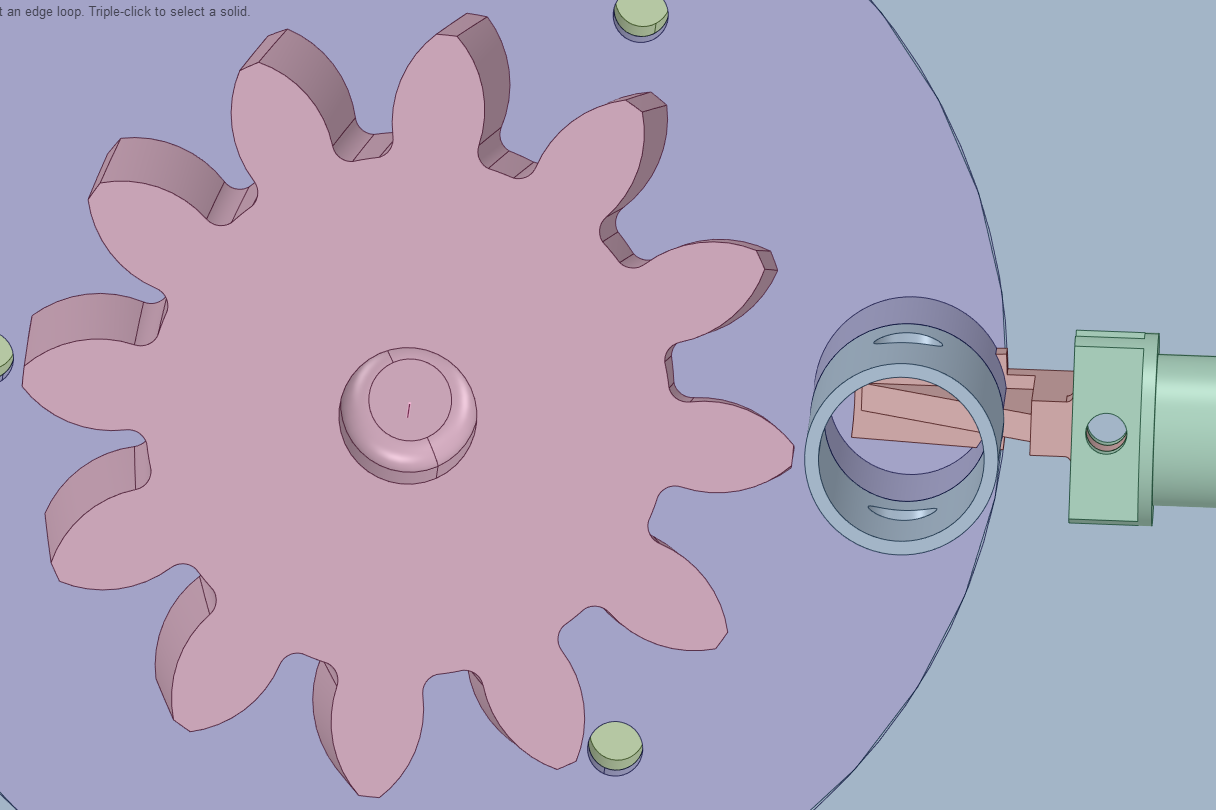
\includegraphics[width=.7\textwidth]{figuras/estrutura/Design/engrenagem_mangueira.png}
        \caption{Porção Inferior do contêiner com um exemplo de engrenagem.}
        \label{fig:mangueira_engrenagem}
    \end{figure} 

Na engrenagem modelada foi utilizado um ângulo de hélice ($\psi$) de 20$^{\circ}$ e um ângulo de pressão ($\phi$) também de 20$^{\circ}$, além de uma quantidade de dentes ($N_G$) de 21 dentes e um módulo ($M$) de 2 mm. A escolha do ângulo de hélice foi baseada nos valores padrão utilizados na indústria, a escolha do ângulo de pressão, além de baseada em valores usuais, foi considerado também seu rendimento de transmissão ($\eta_T$) estimado em 85,9$\%$ para um coeficiente de atrito $f$ = 0,05 entre o par sem-fim. O número de dentes adotado foi de 21 dentes, que seria o mínimo para uma coroa do par sem-fim, para evitar interferência, considerando o ângulo de pressão escolhido. A escolha do módulo (também chamado de módulo aparente ou módulo frontal) foi feita considerando os valores para tamanho de fresa, caso sua manufatura fosse feita por usinagem, e também o diâmetro da engrenagem com base no número de dentes. \cite{shigley2005}

As Eq. \ref{eqengrenagem1} a \ref{eqengrenagem8} representam as relações dimensionais para engrenagens helicoidais \cite{shigley2005} e foram utilizadas para determinar os outros parâmetros necessários supracitados, afim de determinar a geometria das engrenagens. 

\begin{alignat}{8}
\label{eqengrenagem1}
    D_p & = N_G \cdot M & [\text{mm}]\\
\label{eqengrenagem2}
    D_e & = D_p + 2 \cdot M & [\text{mm}] \\
\label{eqengrenagem3}
    p_t & = \frac{D_P \cdot \pi}{N_G} & [\text{mm}] \\
\label{eqengrenagem4}
    p_n & = p_t \cdot \cos{\psi} & [\text{mm}] \\
\label{eqengrenagem5}
    p_x & = \frac{p_t}{\tan{\psi}} & [\text{mm}]\\
\label{eqengrenagem6}
    \phi_t & = tan^{-1}\left(\frac{\tan{\phi}}{\cos{\psi}}\right) & [\text{graus}] \\
\label{eqengrenagem7}
    P_t & = \frac{N_G}{D_p} & [\text{dentes/mm}]\\
\label{eqengrenagem8}
    P_n & = \frac{P_t}{\cos{\psi}} & [\text{mm}]
\end{alignat}


Onde $D_p$ é o diâmetro primitivo, $D_e$ é o diâmetro externo, $p_t$ é o passo circular transversal, $p_n$ é o passo circular normal, é $p_x$ o passo axial além de $P_t$ e $P_n$ serem os passos diametral transversal e normal, respectivamente. $\phi_t$ é o ângulo de pressão transversal. 

Os valores dimensionais calculados para a engrenagem do contêiner, com base nos valores inicialmente estabelecidos, foram:

\begin{itemize}\label{calculo_fuso}
    \item $D_p$ = 42 mm
    \item $D_e$ = 46 mm
    \item $p_t$ = 5,998 mm
    \item $p_n$ = 5,636 mm
    \item $p_x$ = 2,183 mm
    \item $\phi_t$ = 21,17$^{\circ}$
    \item $P_t$ = 0,5 dentes/mm
    \item $P_n$ = 0,532 mm
\end{itemize}

É importante salientar que os valores acima com resolução da ordem de três casas decimais não são parâmetros de construção e, por isso, apresentam esta resolução. São parâmetros geométricos decorrentes de escolhas dimensionais e parâmetros de construção, estes sim com resolução menor e menos algarismos significativos.

%\begin{tabular}{lp{8cm}}
% Diâmetro Primitivo:                    & $D_p$ = 42 mm \\
% Diâmetro Externo:                      & $D_e$ = 46 mm \\
% Passo circular Transversal:            & $p_t$ = 5,998 mm \\
% Passo circular Normal:                 & $p_n$ = 5,636 mm \\
% Passo Axial:                           & $p_x$ = 2,183 mm \\
% Ângulo de Pressão Transversal:         & $\phi_t$ = 21,17$^{\circ}$ \\
% Passo diametral Transversal:           & $P_t$ = 0,5 dentes/mm¨\\
% Passo diametral Normal:                & $P_n$ = 0,532 mm \\
%\end{tabular}


%Acho que podemos incluir dois tópicos referentes ao dimensionamento da engrenagem, e outro depois sobre o dimensionamento do fuso.
\subsection{Dimensionamento do fuso} 


A definição da geometria da engrenagem foi determinante para o dimensionamento do fuso como um parafuso sem-fim. Sua rosca é esquerda, assim como a da engrenagem e seu passo axial ($p_x$) é igual ao passo circular da engrenagem ($p_t$), uma vez que o ângulo entre os eixos de rotação do fuso e da engrenagem é de 90$^{\circ}$. 

O diâmetro primitivo do fuso ($d_W$) pode ser escolhido livremente, desde seja o mesmo diâmetro primitivo da fresa caracol usada para cortar os dentes da engrenagem, caindo no intervalo dado pela Eq. \ref{diamfuso}, para evitar interferência durante a operação. Este intervalo foi apontado na literatura e determinado experimentalmente como uma boa prática. Onde $C$ é a distância entre o eixo de rotação do sem-fim e da engrenagem. \cite{shigley2005}

\begin{equation}
\label{diamfuso}
  \frac{C^{0,875}}{3,0} \le d_W \le \frac{C^{0,875}}{1,7} \quad [\text{mm}]
\end{equation}

Ou seja, o passo axial do sem-fim deve ser 5,998 mm ou, para fins de construção, aproximadamente 6 mm. E, para o diâmetro primitivo do sem-fim ($d_W$) neste caso, tomaremos o valor de 19 mm, dentro do intervalo estabelecido por \ref{diamfuso}.

\begin{alignat}{2}
    \label{passofuso1}
    L & = p_x \cdot N_W \quad & [\text{mm}] \\
    \label{passofuso2}
    \lambda & = tan^{-1}\left(\frac{L}{\pi \cdot d_W}\right) \quad & [\text{graus}]
\end{alignat}

Assim, utilizando as Eq. \ref{passofuso1} e \ref{passofuso2} e considerando um fuso com 4 entradas ($N_W$ = 4) –  ou seja, cada volta do parafuso move 4 dentes da engrenagem, resultando em uma relação 5,25:1 entre fuso e engrenagem – os parâmetros geométricos de avanço ($L$) e ângulo de avanço ($\lambda$) para o fuso são apresentados a seguir.

\begin{itemize} 
    \item $L$ = 24 mm
    \item $\lambda$ = 21,90$^{\circ}$
\end{itemize}

Para este valor de $\lambda$, o ângulo de pressão ($\phi_n$) ideal é de 20$^{\circ}$ e o adendo e dedendo ideais são de 2,210 mm e 2,210 mm, respectivamente, de acordo com a Tab. \ref{shigley13-5}.

\begin{table}[!htb]
     \centering
     \caption{Ângulos de pressão recomendados e profundidades de dentes para engrenagens sem-fim. Retirado de: \cite{shigley2005}}
    \centering
     \begin{tabular}{|C{3,5cm}|C{3,7cm}|C{1,6cm}|C{2cm}|}
     \rowcolor[HTML]{A8DADC}
       \hline
      \textbf{Ângulo de avanço $\lambda$ [graus]} &
      \textbf{Ângulo de pressão $\phi_n$ [graus]} &
       \textbf{Adendo $a$} &
        \textbf{Dedendo $b_G$} \\ \hline
        0-15 & 14,5 & 0,3683$p_x$ & 0,3683$p_x$ \\ \hline
         15-30 & 20 & 0,3683$p_x$ & 0,3683$p_x$ \\ \hline
        30-35 & 25 & 0,2865$p_x$ & 0,3314$p_x$ \\ \hline
        35-40 & 25 & 0,2546$p_x$ & 0,2947$p_x$ \\ \hline
        40-45 & 30 & 0,2228$p_x$ & 0,2578$p_x$ \\ \hline
        \end{tabular}
     \label{shigley13-5}
\end{table}

Por fim, podemos realizar a análise de forças no sem-fim, para simular as cargas de operação e obter as tensões por análises de elementos finitos a fim de que o material se mantenha no regime elástico e evite também a falha por fadiga, considerando a tensão à qual o par de engrenagens será submetido.

Vamos considerar que o motor de passo opere a uma velocidade de 158 rpm, suficiente para girar o fuso a aproximadamente 30 rpm, considerando a razão de redução de 5,25:1. A potência máxima do motor em questão é de 4,80 W (ou 0,00643 hp, valor utilizado na Eq. \ref{eqpotenciaeng}). Vamos chamar também um eixo paralelo ao eixo de rotação da engrenagem de “z”, um eixo paralelo ao eixo de rotação do sem-fim de “x” e o eixo perpendicular a ambos de “y”.

Começando pela determinação da velocidade no círculo primitivo do par sem-fim ($V_W$) a partir da Eq. \ref{wormspeed}, onde as medidas são expressas em polegadas e $n_W$ é a velocidade (em rpm) do fuso:

\begin{equation}
    \label{wormspeed}
    V_W = \frac{\pi \cdot d_W \cdot n_W}{12} \quad [\text{pol/min}]
\end{equation}

Assim, a velocidade encontrada no círculo primitivo do fuso, convertida para o SI, é 0,157 m/s. Aplicando a equação de potência (Eq. \ref{eqpotenciaeng}), onde H é a potência transmitida pelo fuso em hp e cujo resultado é dado em lbf.

\begin{equation}
    \label{eqpotenciaeng}
    W^z = \frac{33000 \cdot H}{V_W} \quad [\text{lbf}]
\end{equation}

Temos que a força no eixo “z” ($W^z$) adotado anteriormente é, após conversão das unidades, 30,5 N. As demais componentes dependem do coeficiente de atrito entre o par sem-fim, para tanto, consideramos o torque máximo do motor de passo (0,40 N$\cdot$m) depois da multiplicação pela relação (2,1 N$\cdot$m). O coeficiente máximo de atrito (f) entre um par sem-fim de poliamida (\textit{Nylon}), submetido a este torque, de acordo com \cite{starzhinsky2013}, seria de 0,12. 

As equações \ref{compforc},  \ref{compforcy} e \ref{compforcx} são utilizadas para determinar as componentes da força atuante no contato do par sem-fim.

\begin{alignat}{3}
    \label{compforc}
    W & = \frac{W^z}{\cos{\phi_n}\cdot\sin{\lambda}+f\cdot \cos{\lambda}} & \quad [\text{N}] \\
    \label{compforcy}
    W^y & = W \cdot \sin{\phi_t} & \quad [\text{N}] \\
    \label{compforcx}
    W^x & = W (\cos{\phi_n} \cdot \cos{\lambda} - f \cdot \sin{\lambda}) & \quad [\text{N}]
\end{alignat}

Assim, as magnitudes das componentes da força que atua no contato são:

\begin{itemize}
    \item $W^z$ = 30,50 N
    \item $W^y$ = 23,80 N
    \item $W^x$ = 54,60 N
\end{itemize} 

Aplicando estas condições a ambos os sólidos, feitos de poliamida, e utilizando as propriedades mecânicas mínimas descritas na Tab. \ref{tab:PropPA6}, chegou-se aos resultados apresentados nas Fig. \ref{fig:tensaofuso} e \ref{fig:tensaoeng} da Análise numérica.

A máquina irá operar numa temperatura ambiente entre 20-30 $^{\circ}$C, a maior velocidade linear à qual o par sem-fim será submetido é de aproximadamente 0,16 m/s no círculo primitivo do fuso e a tensão equivalente von Mises nos dentes da Engrenagem está em uma faixa entre 20 MPa e 30 MPa. Com esses dados, podemos inferir que a engrenagem está projetada para uma faixa de operação de vida infinita sem necessidade de lubrificação e seu desgaste após 10$^7$ ciclos está em uma faixa de apenas 20-23 $\mu$m de acordo com \cite{starzhinsky2013}.

De maneira resumida, os parâmetros geométricos da engrenagem do eixo de rotação da rampa seletora, assim como os parâmetros do seu par sem-fim (fuso), estão apresentados na Tab. \ref{tab:resumo_p}. Os parâmetros apresentados na Tab. \ref{tab:resumo_p}, em conjunto com as equações descritas nesta seção, são suficientes para calcular quaisquer outros parâmetros. A omissão destes outros parâmetros, além da simplificação na apresentação dos dados, ocorre porque eles não são necessários à seleção de ferramentas e processos de fabricação dos componentes (Fresagem Renânia por fresa caracol).

\begin{table}[!htb]
     \centering
     \caption{Resumo dos parâmetros geométricos da engrenagem e do seu par sem-fim (fuso).}
    \centering
     \begin{tabular}{|l|c|c|c|}
     \rowcolor[HTML]{A8DADC}
       \hline
       \multicolumn{1}{|c|}{\textbf{Parâmetro}} &
      \multicolumn{1}{c|}{\textbf{Unidade}} &
       \textbf{Fuso} &
        \textbf{Engrenagem} \\ \hline
        Ângulo de hélice ($\Psi$) & [graus] & 20 & 20 \\ \hline
        Ângulo de Pressão ($\phi$) & [graus] & N/A & 20 \\ \hline
        Ângulo de Pressão normal ($\phi_n$) &[graus] & 20 & N/A \\ \hline
        Ângulo de Avanço ($\lambda$) & [graus]& 21,9 & N/A \\ \hline
        Diâmetro Primitivo ($D_P$) & [mm] & N/A & 42 \\ \hline
        Diâmetro Primitivo ($d_W$) & [mm] & 19 & N/A \\ \hline
        Módulo ($M$) & [mm]& 2 & 2 \\ \hline
        Avanço ($L$) & [mm]& 24 & N/A \\ \hline
        Rosca & \multicolumn{1}{c|}{N/A} & Esquerda & Esquerda \\ \hline
        Número de Dentes ($N_G$) & \multicolumn{1}{c|}{N/A} & N/A & 21 \\ \hline
        Número de Entradas ($N_W$) & \multicolumn{1}{c|}{N/A} & 4 & N/A \\ \hline
        \end{tabular}
     \label{tab:resumo_p}
     
\end{table}


\section{Análises Numéricas}

Foi escolhido o software \textit{ANSYS R19.2} para fazer a análise dos desenhos gerados no \textit{CATIA V5R21} e nas plataformas auxiliares do \textit{ANSYS} com \textit{DesignModeler} e \textit{SpaceClaim}. As análises numéricas compreendem quatro vertentes, sendo a primeira a modelagem da interação fuso-engrenagem, a segunda como uma análise dos modos de vibração do subgrupo simplificado, a terceira sendo a simulação estática do conjunto do subgrupo estrutural e da estrutura tubular de sustentação do sistema e a quarta será uma análise térmica do subgrupo estrutural com um volume de controle.

\subsection{Elementos da malha}
%\subparagraph*{$\bullet$ Elementos da malha} \hfill

%O primeiro estudo realizado foi a análise dos elementos de malha, responsáveis pela transformação de um problema contínuo e descrito por equações diferenciais analíticas para geometrias simples, substituído por um conjunto de volumes finitos representados por nós e malhas numéricas. 

%No geral, iremos fazer a escolha de densidade dos elementos de malhas variada, conhecidas como malhas não-estruturadas, onde regiões críticas terão mais nós e regiões complementares terão menos elementos \cite{malha}. Um elemento fundamental para a análise das malhas é a qualidade, onde quanto maior o refino mais preciso é o resultado aproximado pela malha e temos sua representação nas Fig.

Malhas são o método de transformação de um problema contínuo descrito por equações diferenciais para um conjunto de volumes finitos representados por nós e elementos numéricos.

Como forma de validação dessas malhas, temos os parâmetros conhecidos como métricas os quais são responsáveis por caracterizar a qualidade da malha, e para fim de exemplificação para abordagem realizada nesse estudo, serão consideradas as métricas de \textit{Aspect Ratio}, \textit{Smoothness} e \textit{Orthogonality} \cite{luiz_malha} para a construção do \textit{Element Quality} do \textit{ANSYS}.

\textit{Aspect Ratio} ou razão de aspecto caracteriza a razão entre a maior e a menor aresta do elemento. Idealmente, o valor da razão de aspecto deveria ser 1 para garantir os melhores resultados, ou em outras palavras, uma maior simetria de arestas.

\textit{Smoothness} ou suavização é uma métrica que está relacionada com a transição no tamanho dos volumes adjacentes na malha. Esta transição deve ser suave para evitar erros de truncamento nas aproximações numéricas para cálculo de fluxos e gradientes.

Por fim, \textit{Orthogonality} ou ortogonalidade qualifica desvio do ângulo entre o vetor que conecta o centro dos volumes adjacentes e o vetor normal à superfície entre eles. É a métrica responsável por melhor caracterizar a penalização do operador gradiente em uma malha.
A Fig. \ref{fig:mesh} ilustra a relação entre volumes e nós para tais parâmetros.

%\begin{figure}[htp]
%\centering
%\begin{subfigure}[b]{0.5\linewidth} 
%\centering
%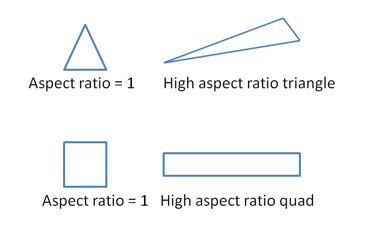
\includegraphics[width=.8\linewidth]{figuras/estrutura/Imagens PC3/Malhas/aspect ratio.png} 
%\caption{\label{fig:ar}\textit{Aspect Ratio}} 
%\end{subfigure}\hfill
%\begin{subfigure}[b]{0.5\linewidth} 
%\centering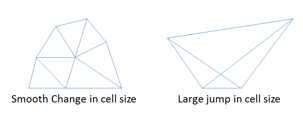
\includegraphics[width=1\linewidth]{figuras/estrutura/Imagens PC3/Malhas/Smoothness.png} 
%\caption{\label{fig:sm}\textit{Smoothness}} 
%\end{subfigure}\vspace{10pt}

%\begin{subfigure}[b]{\linewidth} 
%%\centering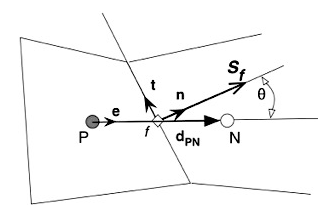
\includegraphics[width=5cm]{figuras/estrutura/Imagens PC3/Malhas/Ortogonalidade.png}
%\caption{\label{fig:or}\textit{ Orthogonality}} 
%\end{subfigure} 
%\caption{Métricas-padrão para análise de Qualidade de Malhas. Fonte: Adaptado de \cite{luiz_malha}} \label{fig:mesh}
%\end{figure} 


\begin{figure}[H]
\centering
\subfloat[\textit{Aspect Ratio}]{\label{fig:ar}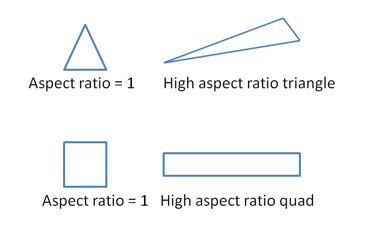
\includegraphics[width=.35\linewidth]{figuras/estrutura/Imagens PC3/Malhas/aspect ratio.png}}\hfill
\subfloat[\textit{Smoothness}]{\label{fig:sm}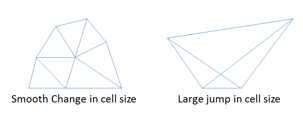
\includegraphics[width=.45\linewidth]{figuras/estrutura/Imagens PC3/Malhas/Smoothness.png}}\par 
\subfloat[\textit{Orthogonality}]{\label{fig:or}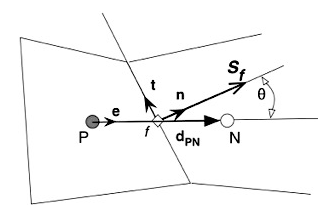
\includegraphics[width=4cm]{figuras/estrutura/Imagens PC3/Malhas/Ortogonalidade.png}}
\caption{Métricas-padrão para análise de Qualidade de Malhas. Fonte: Adaptado de \cite{luiz_malha}}
\label{fig:mesh}
\end{figure}

 Na Fig. \ref{fig:ar} exemplifica-se duas razões de aspecto distintas (malha tetraédrica acima, hexaédrica abaixo para o caso de modelos em três dimensões), na qual a figura com maior simetria apresenta melhor resultado. Para a Fig. \ref{fig:sm}, 
observa-se uma variação de comprimento sutil entre volumes adjacentes localizados na representação à esquerda e na direita uma transição mais brusca (todos os elementos têm formas tetraédricas para modelagem 3D). E concluindo, a Fig. \ref{fig:or} ilustra uma malha com baixa não-ortogonalidade, mas que irá sofrer com a difusão numérica de erros (elementos hexaédricos em 3D).  
Para critério de avaliação das malhas, optou-se por utilizar o misto dos resultados dessas e outras métricas presentes na plataforma \textit{ANSYS}, uniformizados com a funcionalidade \textit{Mesh Quality} da mesma, onde os elementos terão uma avaliação final de 0 a 1 de acordo com os resultados das métricas.

Para simulações com baixo numero de nós, será adotado o modelo de alta densidade de elementos uniformes ou malhas estruturadas (elementos hexaédricos), entretanto, para geometrias com alta complexidade, iremos fazer a escolha de densidade dos elementos de malhas variada, conhecidas como malhas não-estruturadas, onde regiões críticas terão mais nós e regiões complementares terão menos elementos (todos tetraédricos) \cite{malha}. Temos o resultado nas Fig. \ref{fig:Malha_eng}, \ref{fig:malha_carc}, \ref{fig:malha_vol} e \ref{fig:malha_sub}.

\begin{figure}[ht]
        \centering
        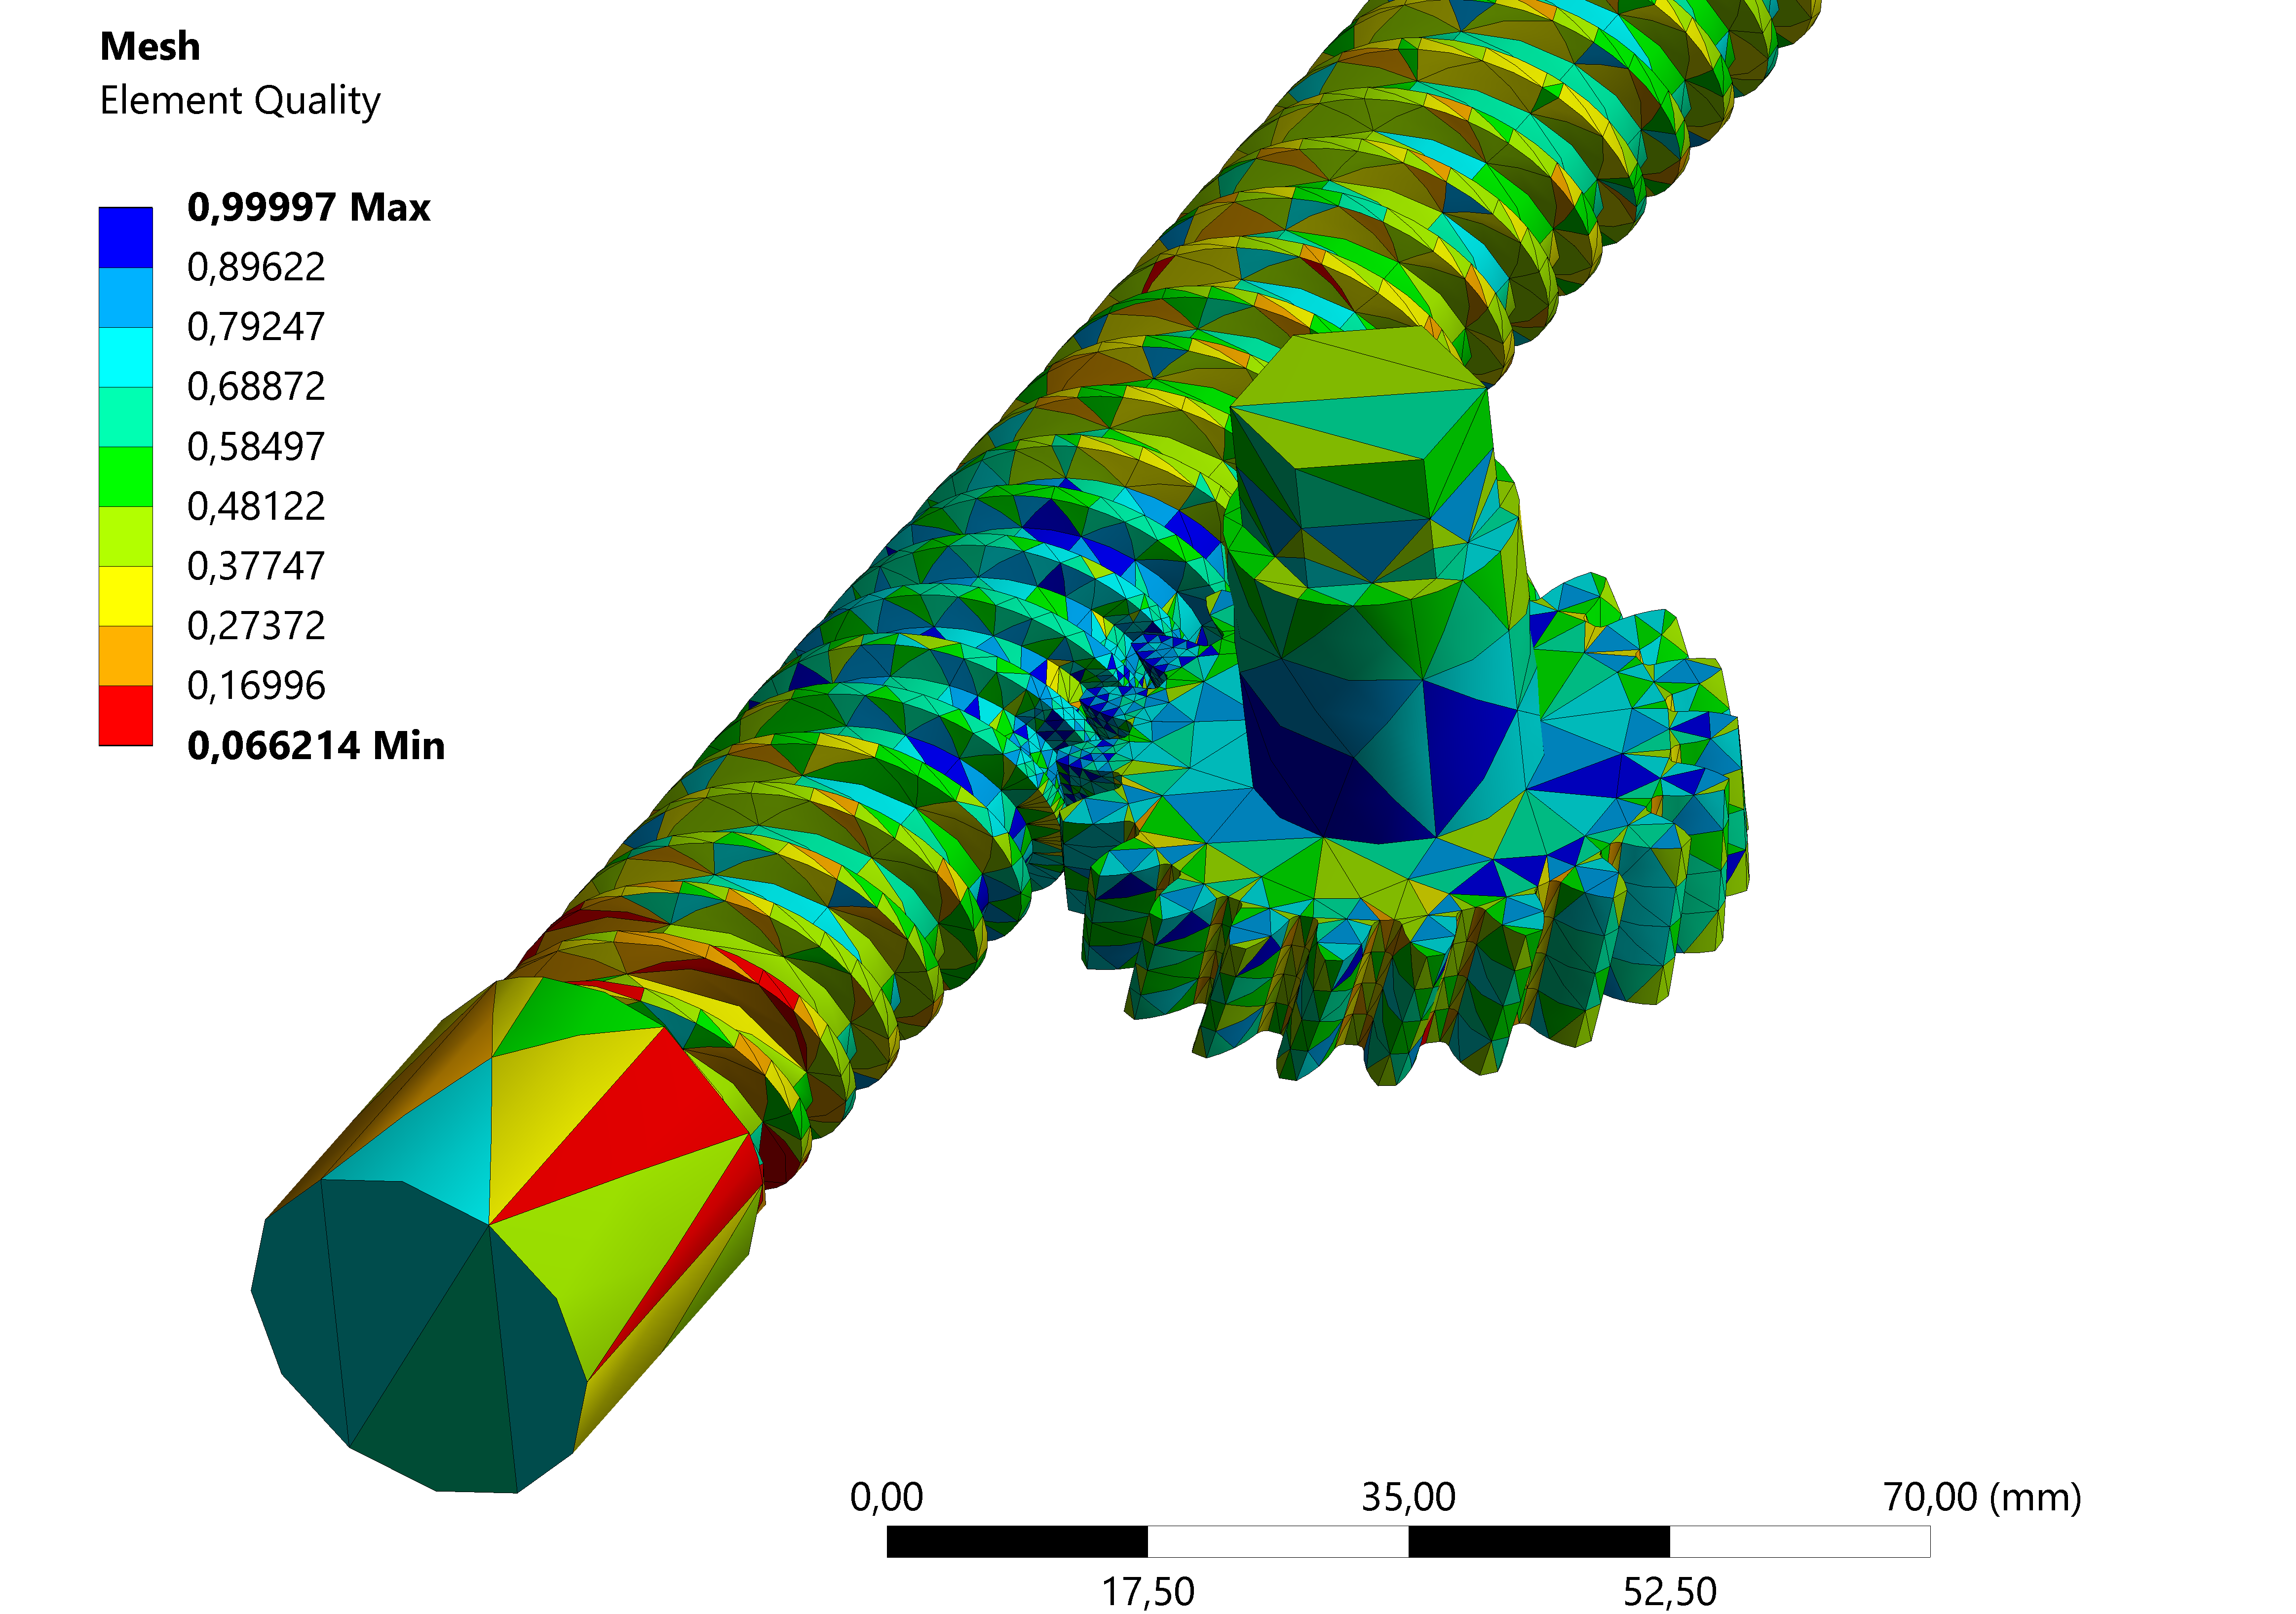
\includegraphics[width=.9\textwidth]{figuras/estrutura/Imagens PC3/Malhas/fuso engrenagem qualidade.png}
        \caption{Qualidade da malha do Fuso com Engrenagem}
        \label{fig:Malha_eng}
    \end{figure}
    
\begin{figure}[H]
        \centering
        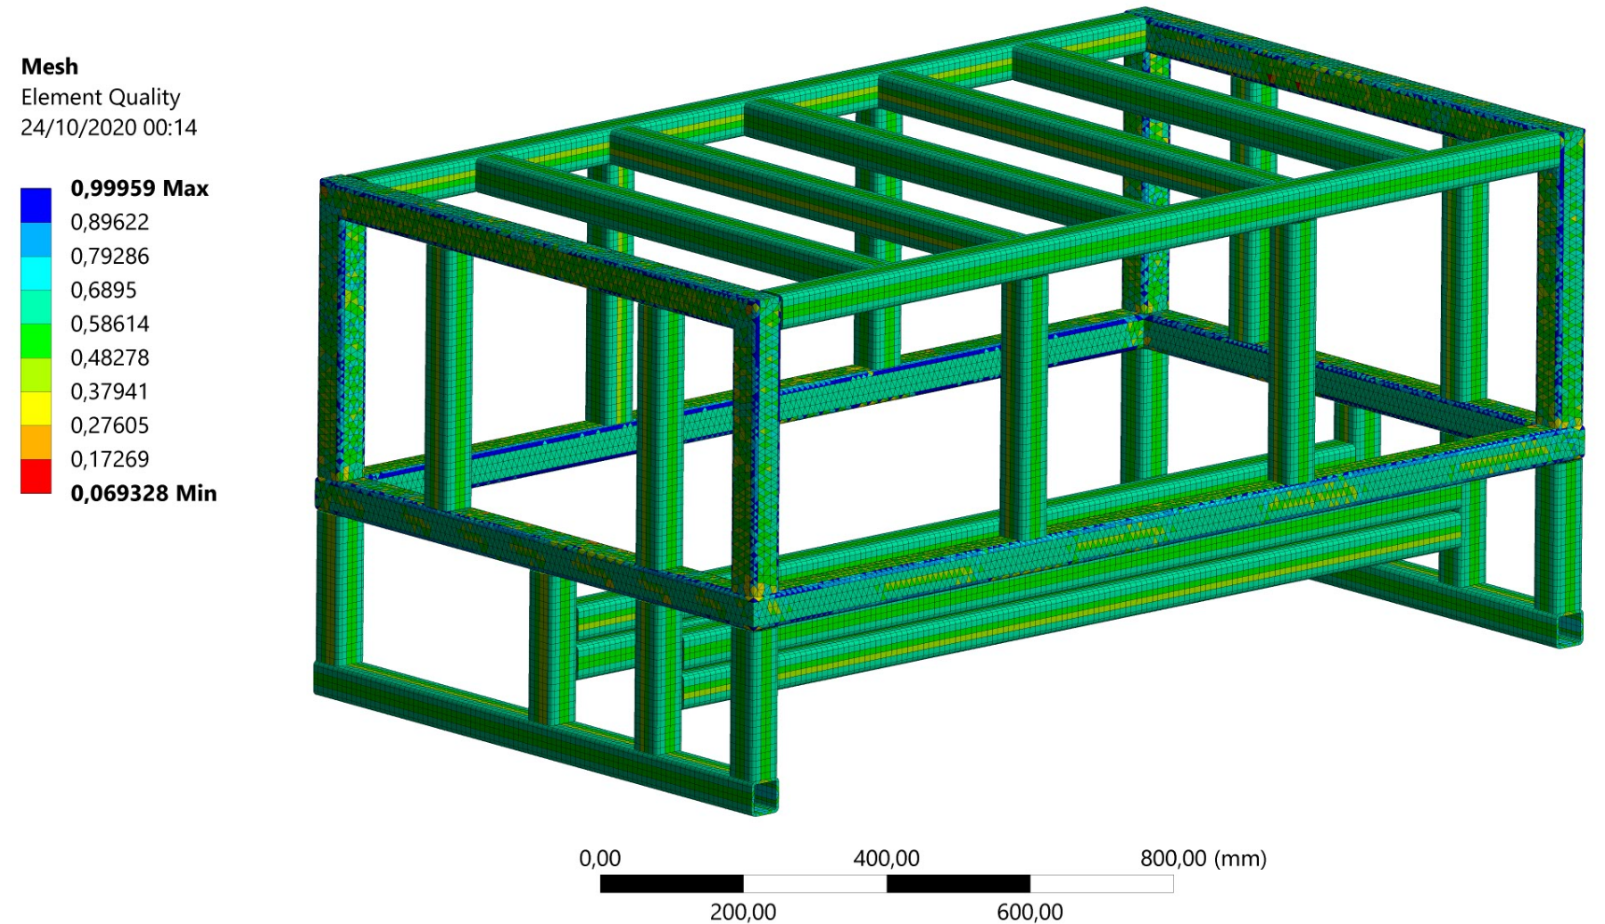
\includegraphics[width=1\textwidth]{figuras/estrutura/Imagens PC3/Malhas/estrutura tubular mesh.png}
        \caption{Qualidade Malha da Estrutura tubular}
        \label{fig:malha_carc}
    \end{figure} 
    
\begin{figure}[H]
        \centering
        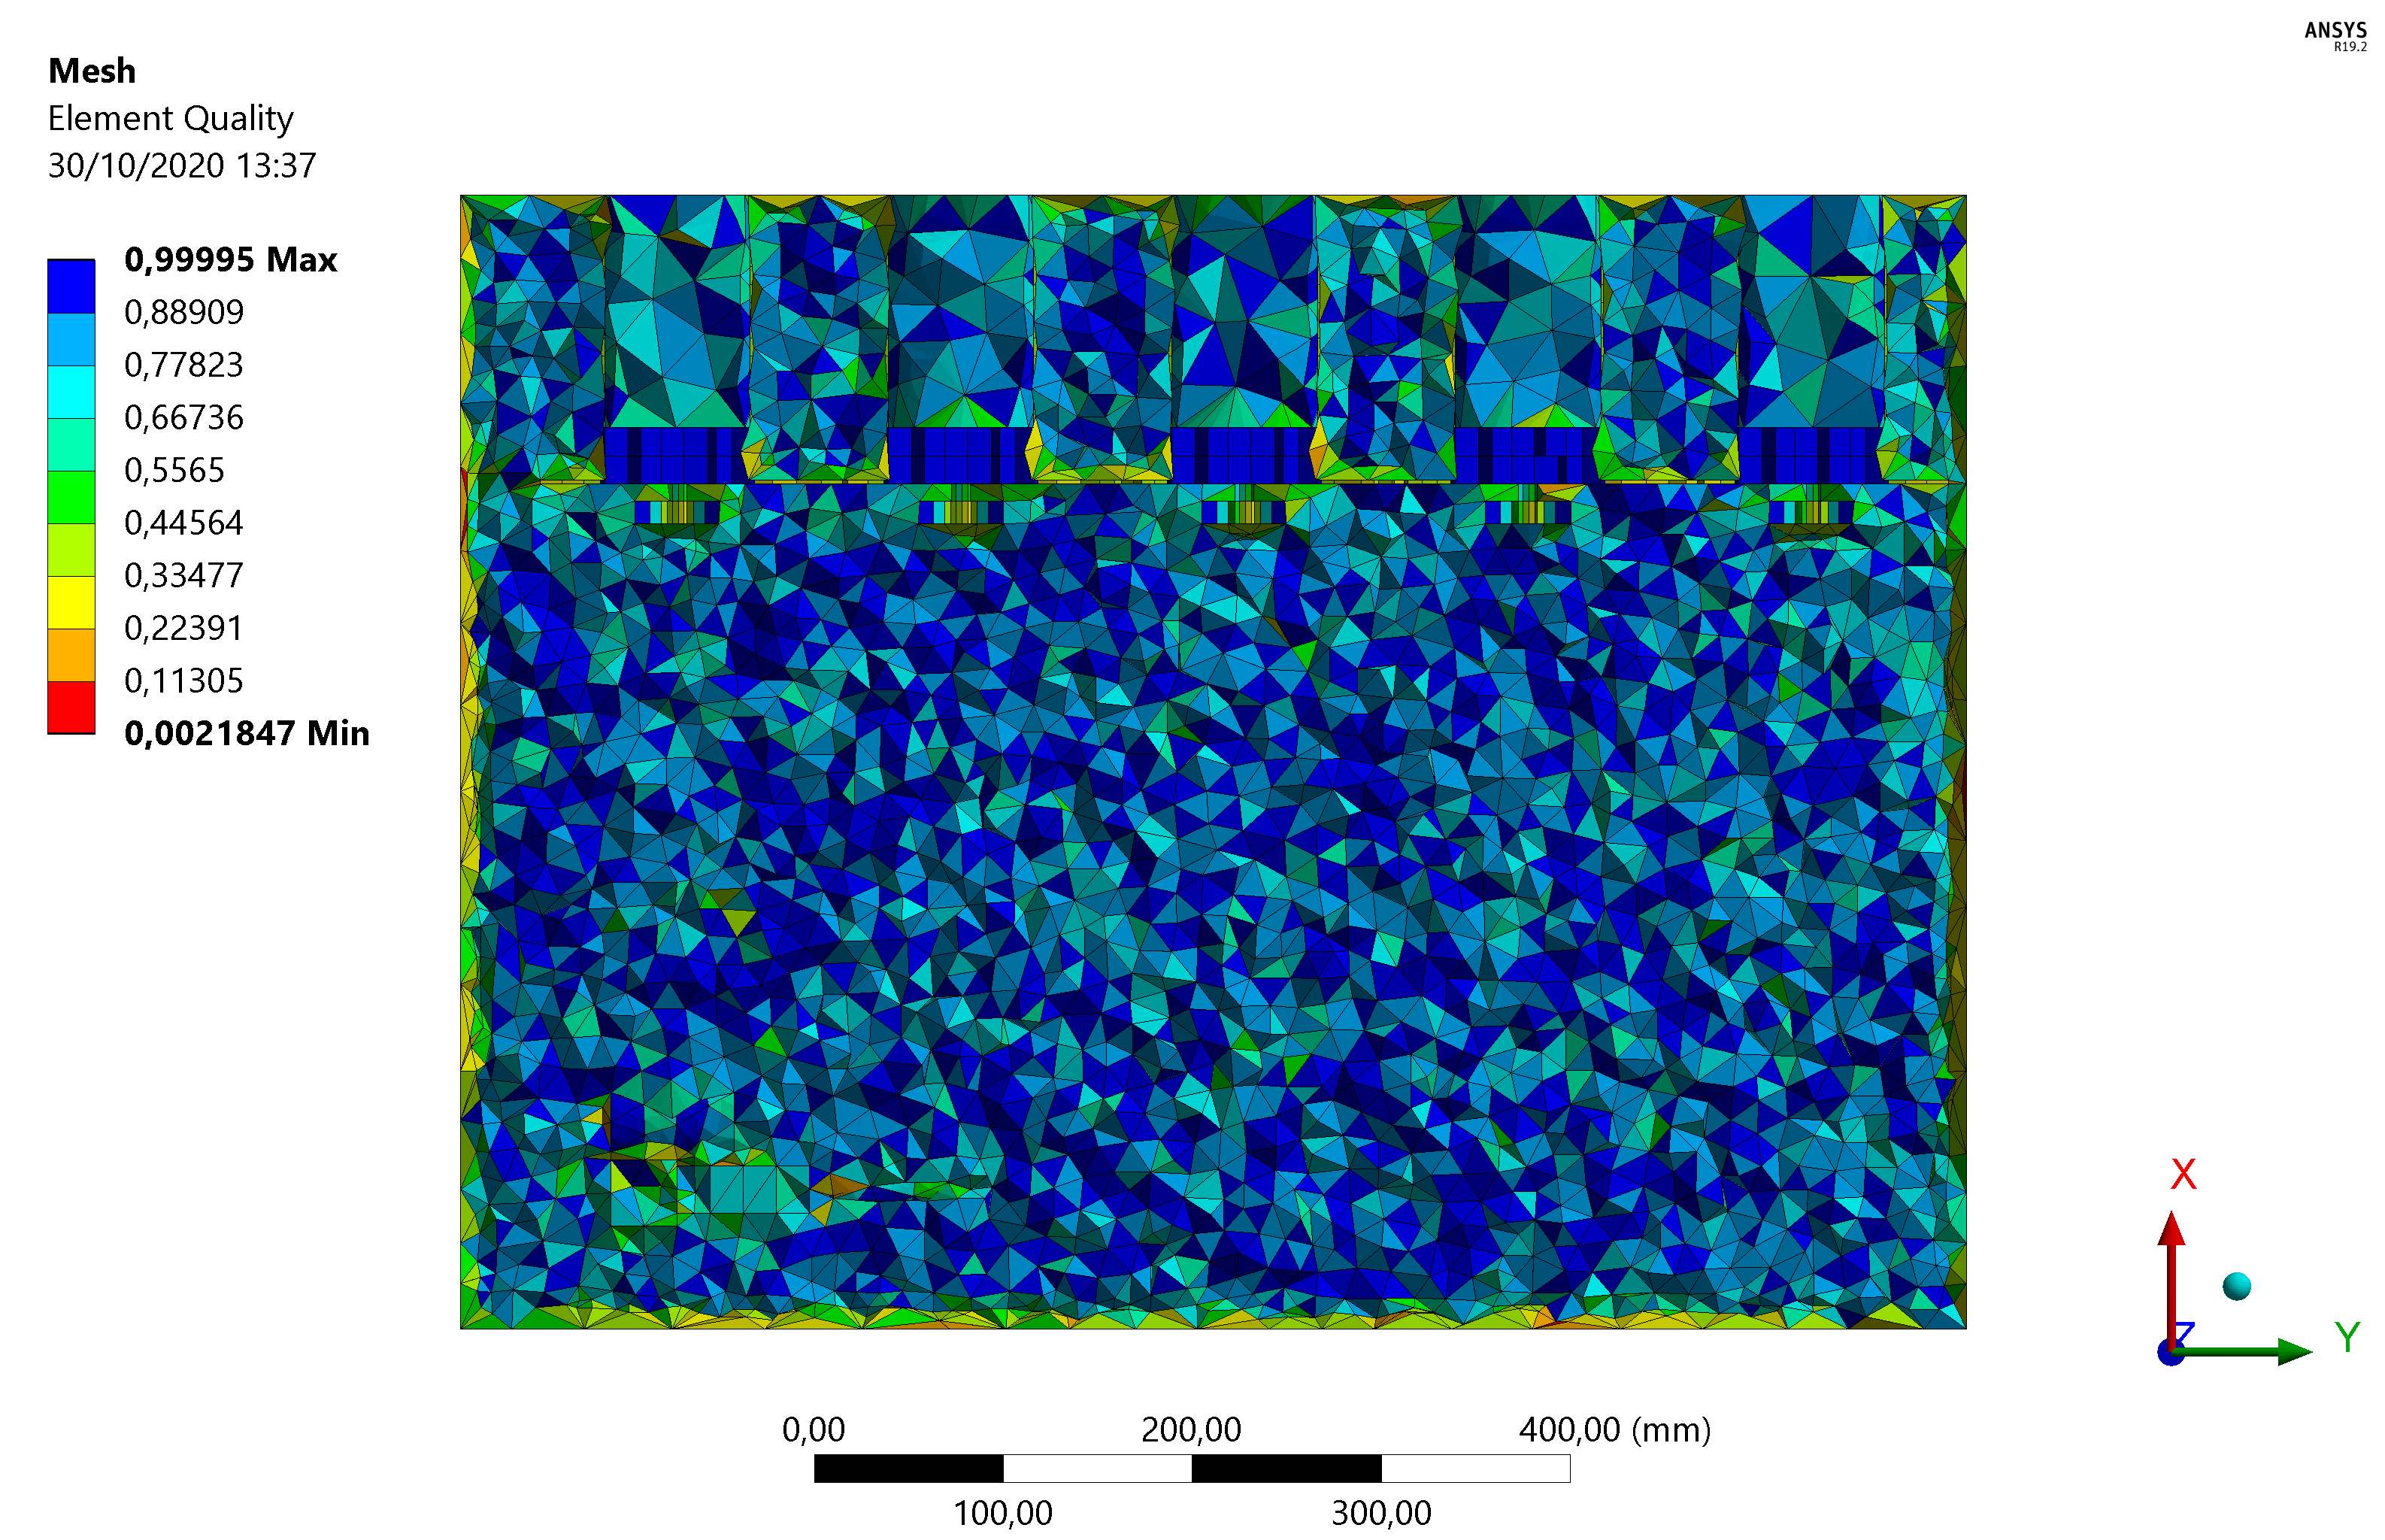
\includegraphics[width=1\textwidth]{figuras/estrutura/InteracaoFusoEng/meshqualityT.png}
        \caption{Qualidade da Malha do volume de controle}
        \label{fig:malha_vol}
    \end{figure}
    
\begin{figure}[H]
        \centering
        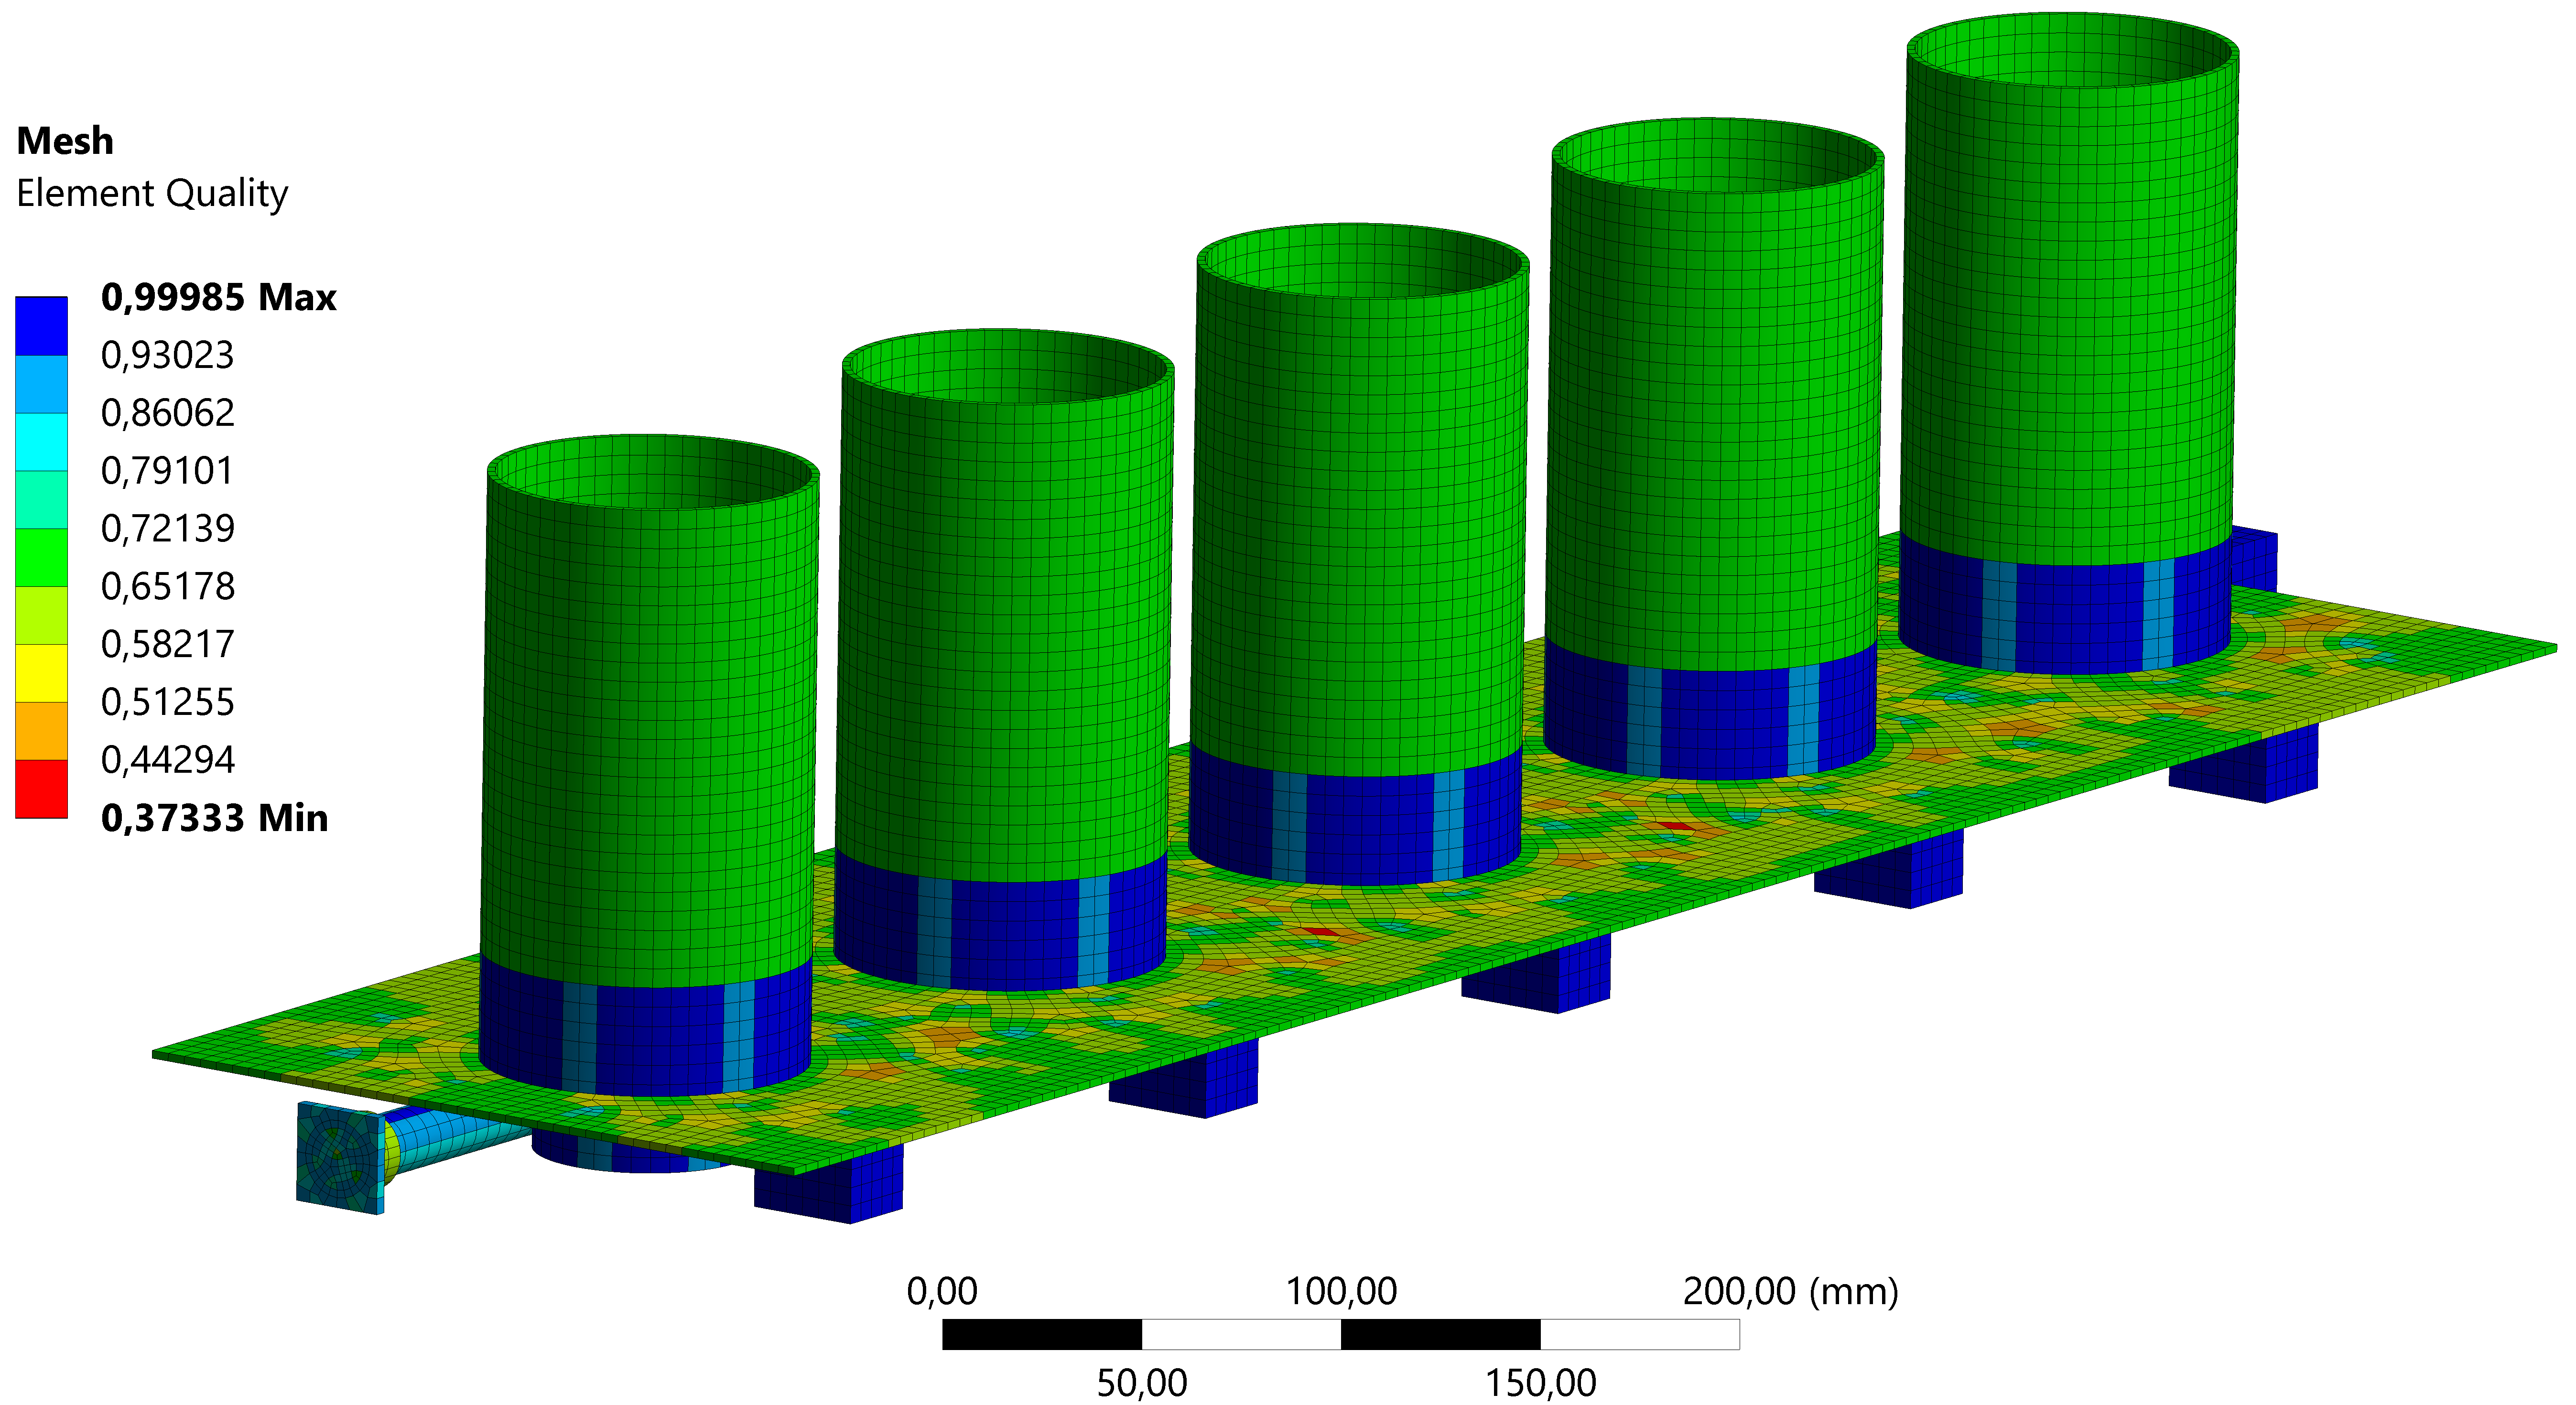
\includegraphics[width=1\textwidth]{figuras/estrutura/Imagens PC3/Malhas/subgrupos malha.png}
        \caption{Qualidade da Malha dos subgrupos}
        \label{fig:malha_sub}
\end{figure}
   
    

%Figura 1, 2 e 3- Malhas do fuso com engrenagem, volume de controle térmico e da estrutura tubular.
Com relação a quantidade de nós e malhas para cada simulação, a Tab. \ref{tab:nos} ilustra a quantidade de nós e elementos por simulação. Temos como conclusão que para geometrias onde existem áreas com grande número de regiões de contato, como por exemplo na geometria do volume de controle, os nós serão melhor aproveitados e por consequência as malhas têm uma qualidade maior para aquele objeto de estudo, de acordo com a análise da qualidade de elemento apresentada.

\begin{table}[ht]
     \centering
     \caption{Número de nós e elementos de malha por simulação}
    \centering
     \begin{tabular}{|C{3cm}|C{3cm}|C{2.5cm}|C{2.5cm}|C{2.5cm}|}
     \rowcolor[HTML]{A8DADC}
       \hline
      \textbf{Malha} &
      \textbf{Engrenagem e Fuso} &
      \textbf{Estrutura Tubular} &
      \textbf{Volume de controle térmico} & \textbf{Subgrupo Estrutural}\\ \hline
        Nós & 163681 & 607876 & 379604 & 157632\\ \hline
         Elementos & 27248 & 164822 & 255686 & 25433 \\ \hline
         
        \end{tabular}
     \label{tab:nos}
\end{table}

Ao mesmo tempo, é perceptível que a qualidade dos elementos encontrada na estrutura tubular e também no o subgrupo estrutural são suficientes para a análise estática e dinâmica estrutural. Com relação ao conjunto fuso-engrenagem, pela complexidade dos objetos em CAD, optou-se por utilizar elementos de qualidade não tão boas quanto os anteriores, pelo alto custo operacional que a análise iria resultar. Conforme já mencionado, para as regiões com contato de interesse, optou-se por uma densidade superior de nós, que é visivelmente clara na Fig. \ref{fig:Malha_eng} e será discutida mais a fundo no estudo da interação do fuso com a engrenagem.


\subsection{Interação Engrenagem com o fuso}
% \subparagraph*{$\bullet$ Interação Engrenagem com o fuso} \hfill   

A análise da interação da engrenagem com o fuso se faz complementar ao estudo do tópico \ref{section:dimensionamento_F_E}, e aqui será abordado o problema estático de reação da engrenagem à rotação do fuso. A primeira etapa seria a determinação das condições de contorno do problema.

Na Fig. \ref{fig:condcontorno}, observamos duas forças aplicadas em sentidos opostos, com a magnitude das componentes determinadas no dimensionamento, representando as forças de reação no contato entre o dente da engrenagem e o fuso.

\begin{figure}[ht]
        \centering
        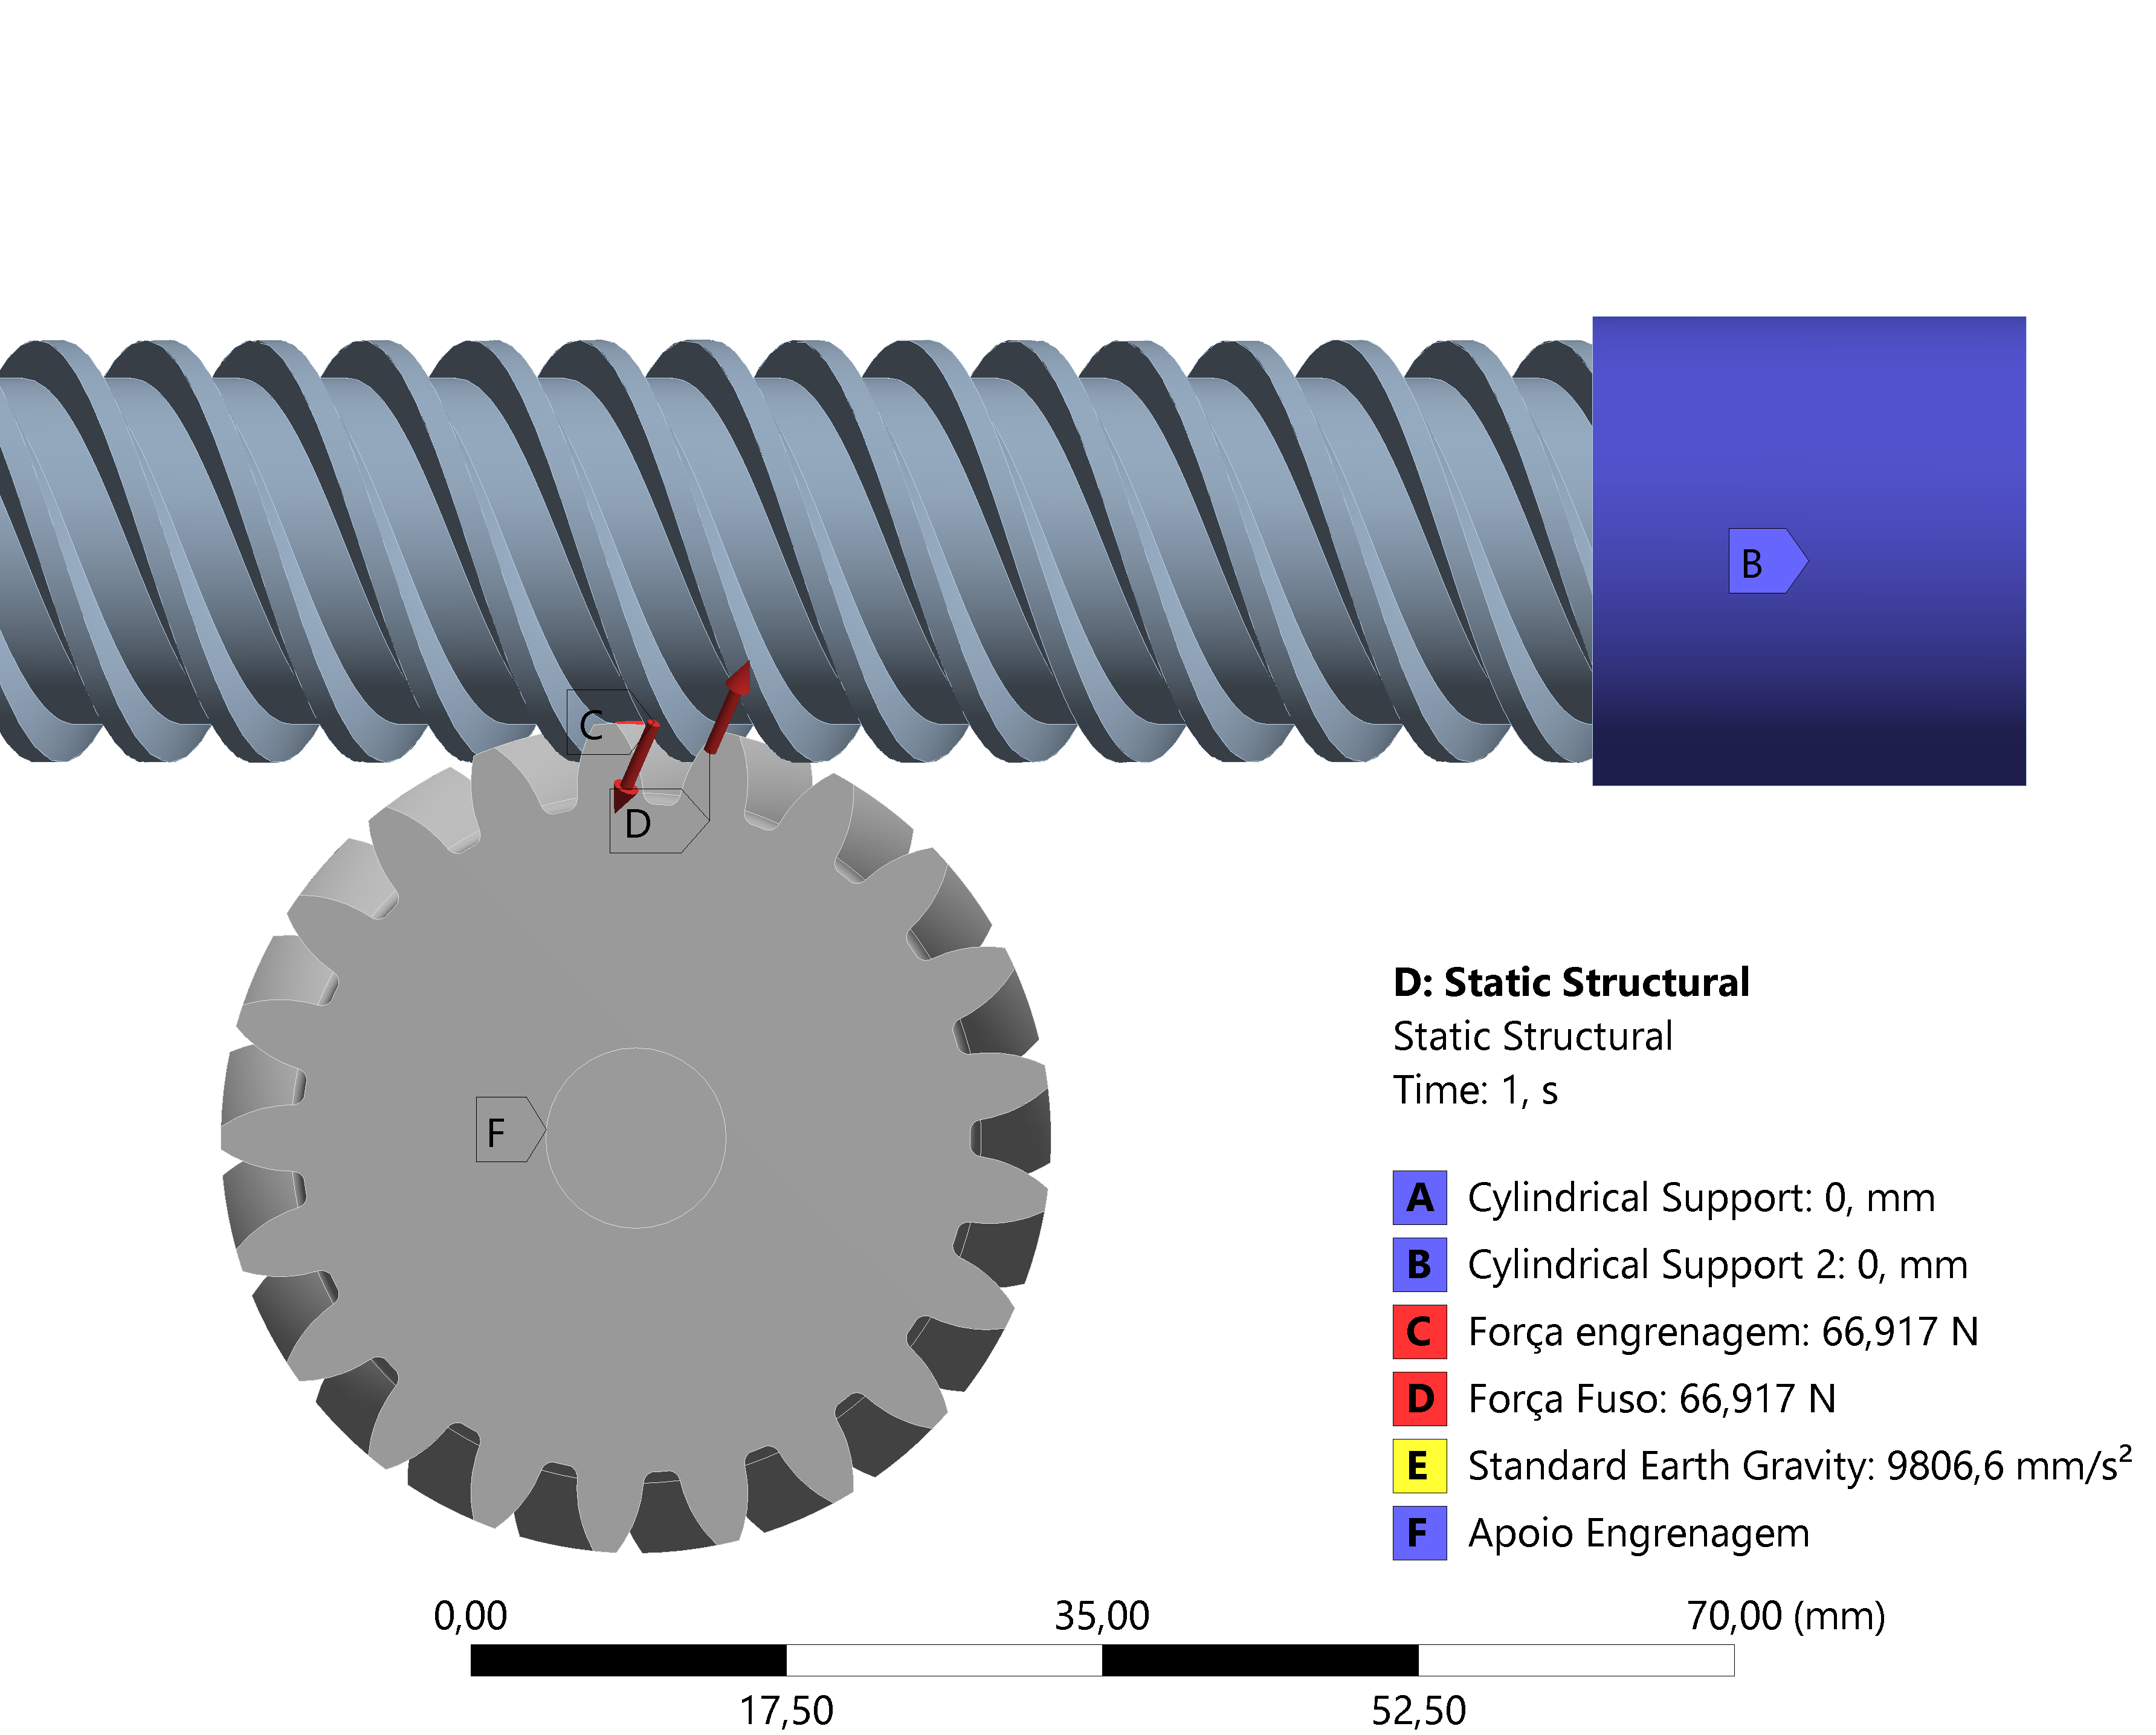
\includegraphics[width=.9\textwidth]{figuras/estrutura/InteracaoFusoEng/PC3 Condicao de contorno.png}
        \caption{Condições de contorno da interação engrenagem fuso}
        \label{fig:condcontorno}
    \end{figure}

Nos resultados apresentados nas Fig. \ref{fig:tensaofuso} e \ref{fig:tensaoeng}, observa-se que as tensões equivalentes von Mises no dente da engrenagem estão em uma faixa entre 20 MPa e 30 MPa. Todavia, no contato com seu par sem-fim, nota-se um único elemento do fuso, localizado na aresta, com uma tensão concentrada de 55 MPa, ainda dentro do limite elástico do material. Consideramos que este valor discordante com a região a sua volta como resultado de uma anomalia pontual da malha.

\begin{figure}[ht]
        \centering
        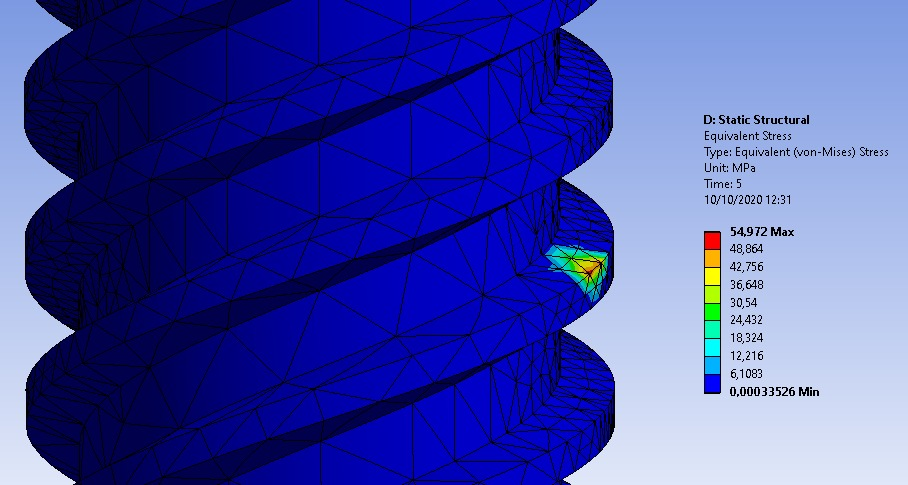
\includegraphics[width=.8\textwidth]{figuras/estrutura/InteracaoFusoEng/tensao fuso.jpeg}
        \caption{Tensões equivalentes von Mises no fuso}
        \label{fig:tensaofuso}
    \end{figure}
    
\begin{figure}[ht]
        \centering
        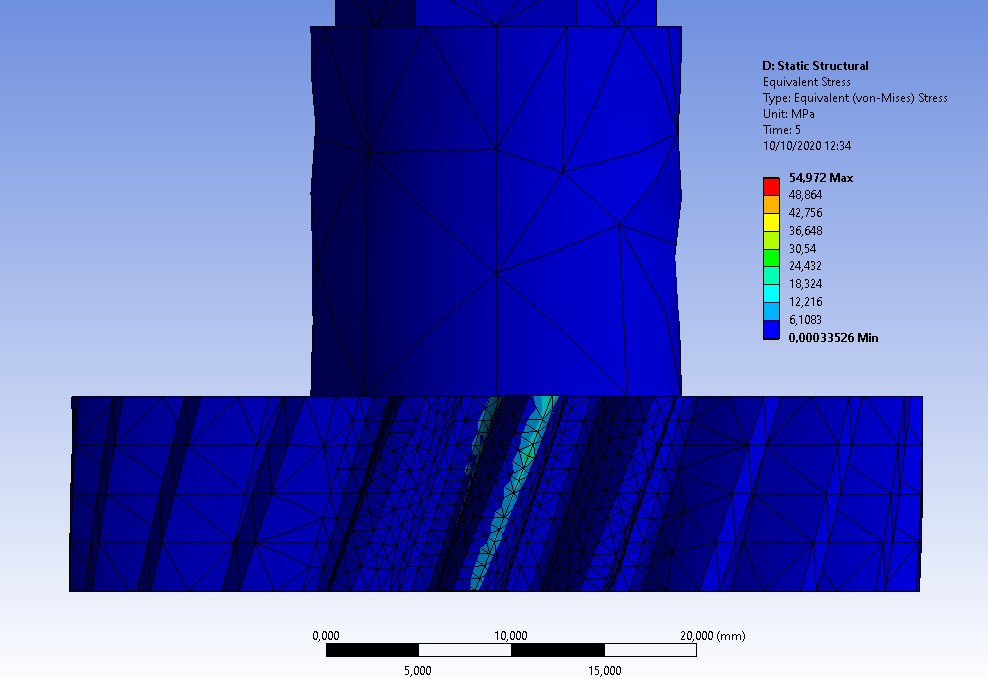
\includegraphics[width=.8\textwidth]{figuras/estrutura/InteracaoFusoEng/tensao engrenagem.jpeg}
        \caption{Tensões equivalentes von Mises na engrenagem}
        \label{fig:tensaoeng}
    \end{figure}    


\subsection{Análise Estrutural}
% \subparagraph*{$\bullet$ Análise Estrutural} \hfill   
    
Para análise das cargas geradas por cada subgrupo, foi feita a escolha da simplificação do sistema para o conjunto mostrado a seguir, onde as estruturas mais complexas foram substituídas por peças de geometria mais simples, como no caso dos motores, caixas quadradas e para o fuso e engrenagens, temos um cilindro do mesmo comprimento do fuso e cinco cilindros com mesma altura e diâmetro das engrenagens (veja a análise térmica em \ref{section:AnaliseTermica} para maiores detalhes da geometria simplificada).


Para o subgrupo de contêineres, foi considerado os efeitos de rotação do fuso (velocidade 158 rpm) e efeito gravitacional nas peças. As condições de contorno foram apoios nas extremidades do fuso, no mancal e nas laterais do subsistema, apoios estes que se refletem em conexões com a estrutura tubular (vide Texto \ref{retorno_tubos_perfilquadrado}). 

As considerações sobre pesos extras no subgrupo estrutural compreenderam um lote com 50 comprimidos de Metformina 850 mg para cada contêiner, totalizando uma força de aproximadamente 0,5 N ou 50g em cada componente cilíndrico. Como se imaginava, a carga aplicada é consideravelmente baixa em relação ao peso próprio da estrutura, que correspondeu a 6,60 kg ou 66 N para cada subgrupo. 

Para os materiais poliméricos, utilizou-se os materiais equivalentes disponíveis na biblioteca \textit{default} do \textit{ANSYS}, com o incremento de dados externos do aço 1020.

No caso da deformação e tensão máximas, observamos um valor total do deslocamento que foi mínimo na estrutura, com magnitude aproximadamente igual a 0,5 mm para os subgrupos. Em relação as tensões, o valor máximo encontrado foi da ordem de 3 MPa na mesa dos contêineres próximo aos apoios com a estrutura tubular, um valor bem abaixo do valor da tensão de escoamento do material da mesa (Tab. \ref{tab:PropA1020}). Os resultados podem ser conferidos pela Fig.\ref{fig:tensao_subgrupo}.

\begin{figure}[ht]
    \centering
    \includegraphics[width=1\textwidth]{figuras/estrutura/AnaliseEstaticaTubular/Tensão total com carga.png}
    \caption{Tensões equivalentes von Mises no subgrupo }
    \label{fig:tensao_subgrupo}
\end{figure}

Com relação à análise estática estrutural do conjunto, foram utilizados os parâmetros levantados anteriormente pela simplificação dos subgrupos e das cargas advindas dos momentos do fuso-engrenagem. Esses parâmetros foram aplicados à estrutura tubular global, em conjunto com forças resultantes da massa dos outros componentes, como Canaletas, suporte das canaletas, mangueiras de silicone, funil, esteira e suas engrenagens, repositório de copos, e chapas da carcaça, com a referência da gravidade sendo 10 m/s$^2$. 

Em seguida, após a aplicação das cargas apresentadas anteriormente em seus devidos pontos de apoio na estrutura tubular, foi feita a análise da força-peso proveniente dos outros quatro subgrupos, em conjunto com a carga de subgrupo calculado anteriormente, na medida que representa um cenário realista de funcionamento da estrutura, onde, enquanto um subgrupo apresenta a reação fuso-engrenagem em funcionamento, os outros quatro restantes se encontram em posição estática. As forças aplicadas na estrutura podem ser visualizadas na Fig. \ref{fig:carga_estruturatubular}.

\begin{figure}[ht]
    \centering
    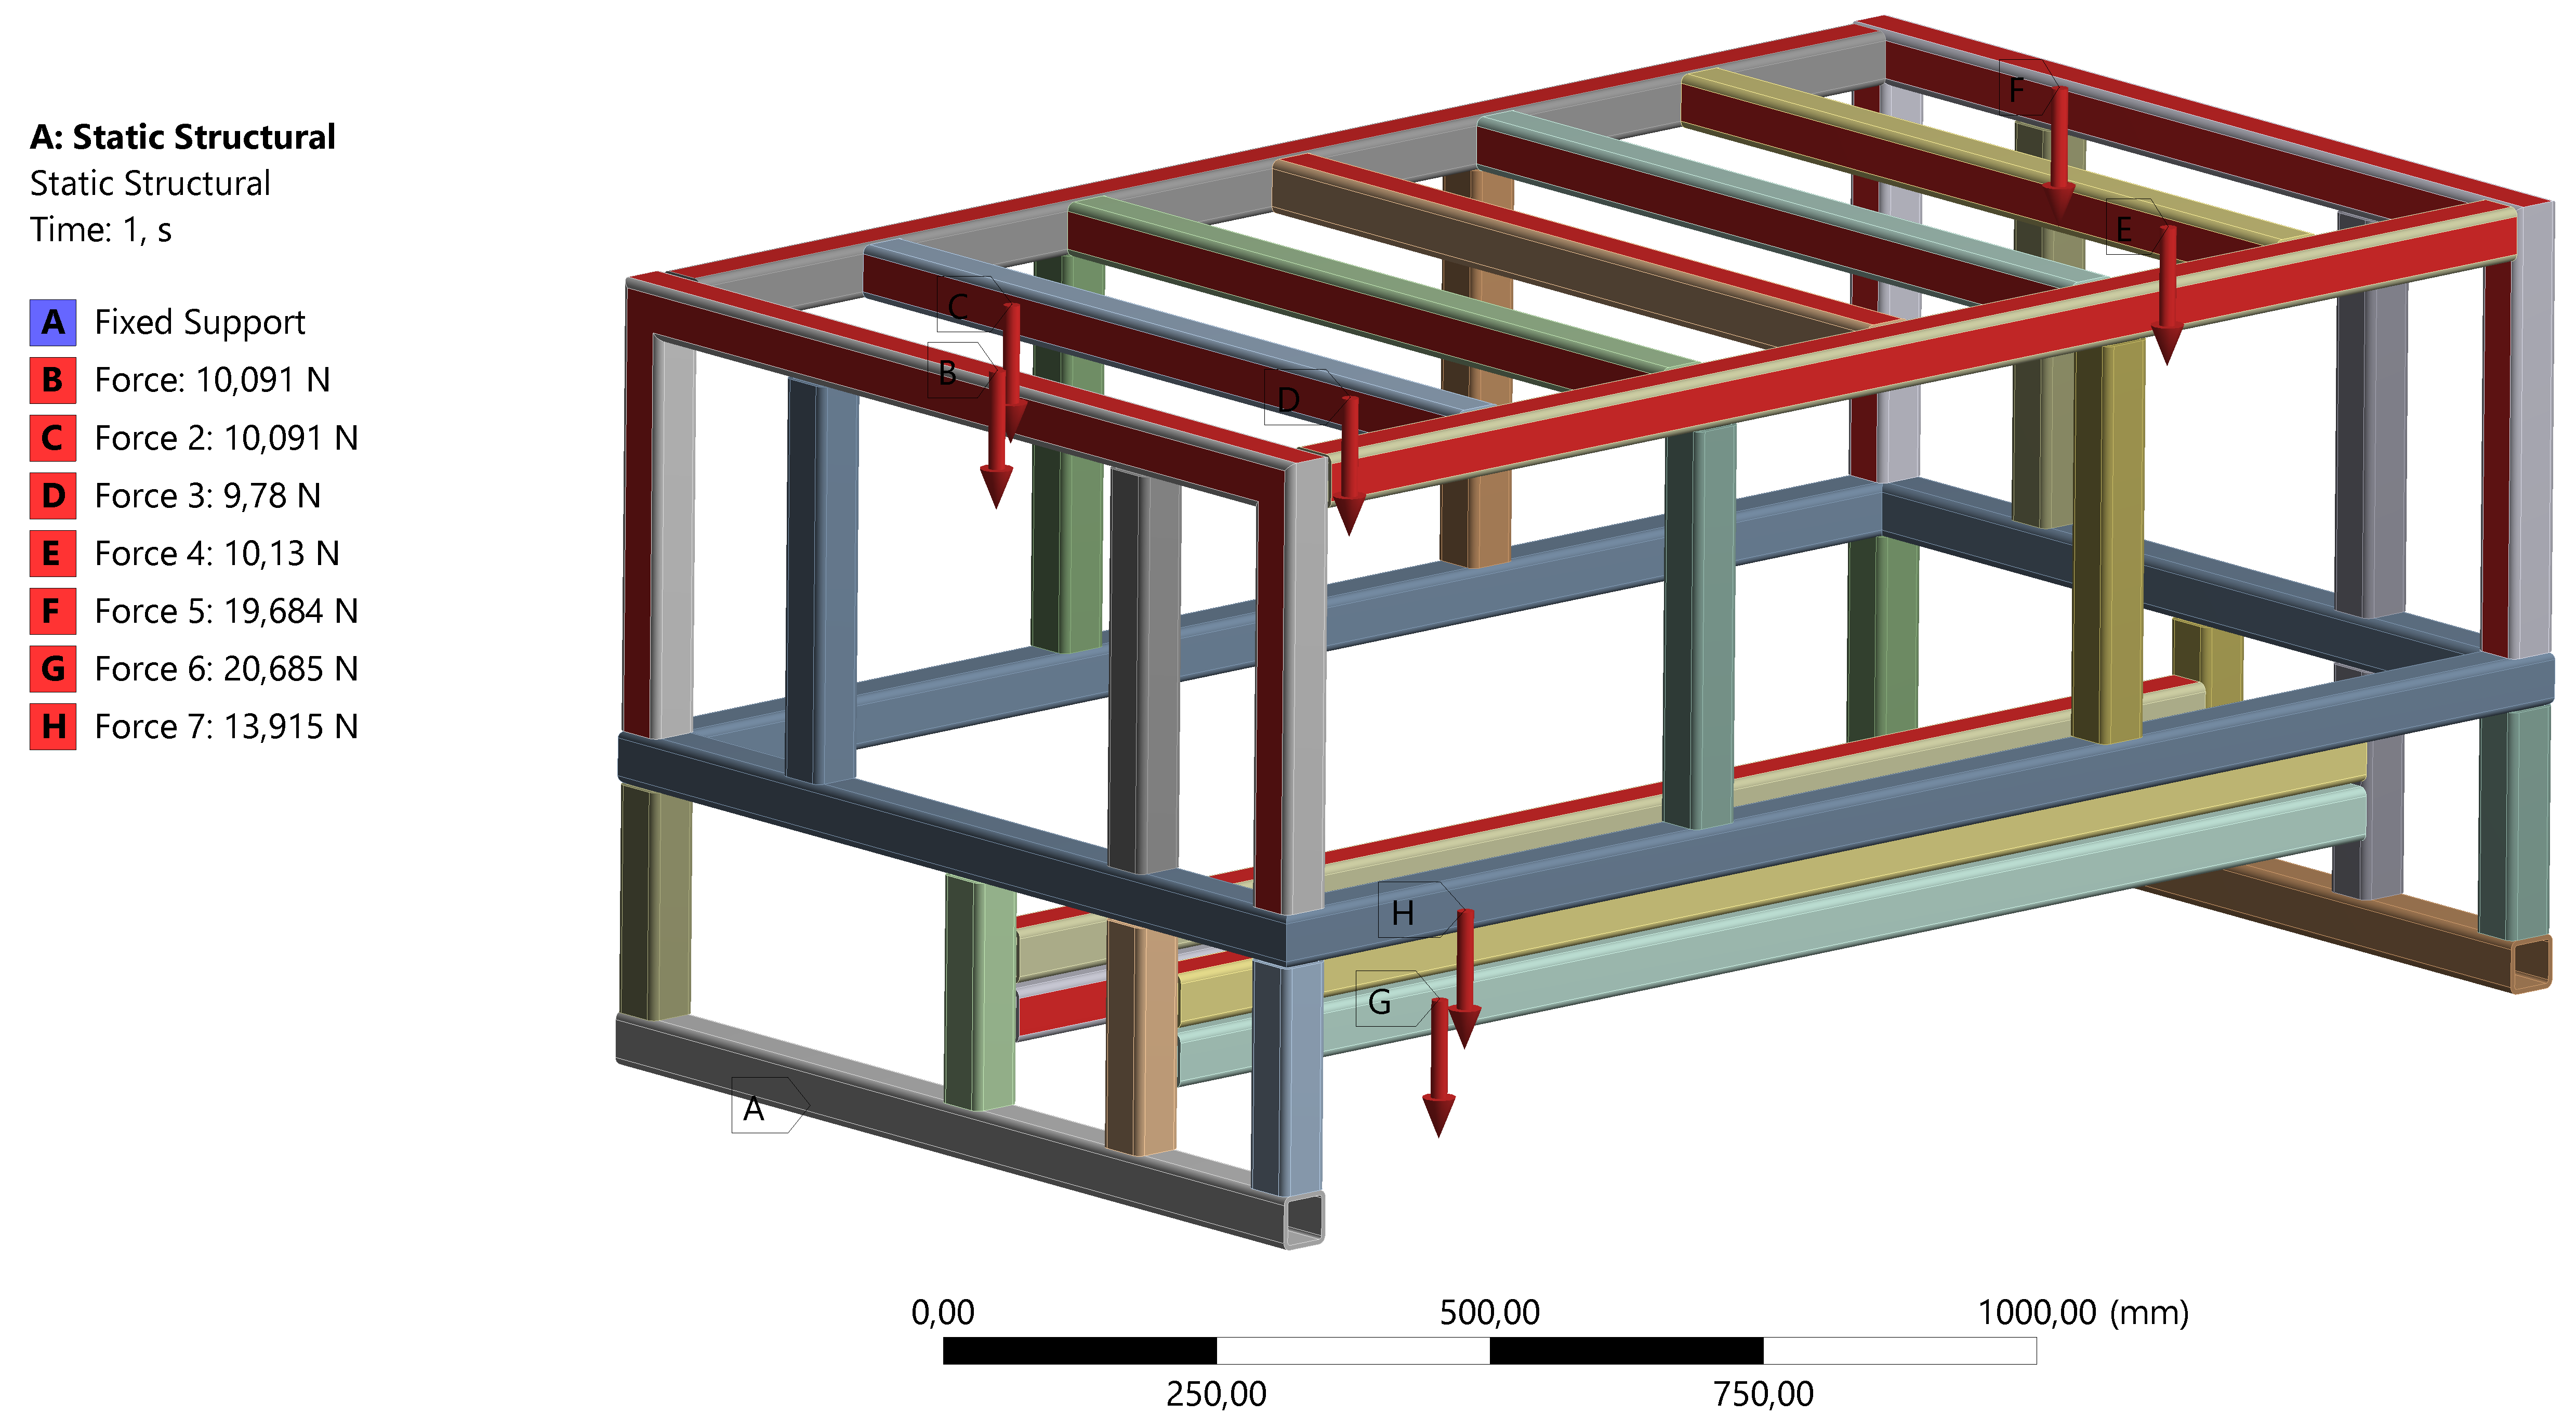
\includegraphics[width=1\textwidth]{figuras/estrutura/AnaliseEstaticaTubular/Cargas_Estrutura.png}
    \caption{Representação das cargas aplicadas à estrutura tubular }
    \label{fig:carga_estruturatubular}
\end{figure}

A explicitação de cada uma dar cargas pode ser observada como:

\begin{itemize}
    \item Forças 1 e 2: 10,09 N, provenientes do resultante dos cálculo do subgrupo com fuso em funcionamento, aplicados nas paredes laterais dos tubos que sustentam este subgrupo, no sentido Z.
    \item Força 3: 9,78 N, correspondente à forças-peso de cada subgrupo, aplicados nas paredes laterais dos tubos que os sustentam, no sentido Z.
    \item Força 4: 10,13 N, correspondente às cargas de força-peso das canaletas, aplicadas em seus devidos subgrupos pelo apoio do suporte das canaletas à estrutura tubular, no sentido Z.
    \item Força 5: 19,68 N, provenientes da força-peso das chapas da carcaça externa, aplicadas em todas as superfícies que apoiam essa estrutura. A força foi aplicada no sentido Z.
    \item Força 6: 20,68 N, proveniente da força-peso derivada do conjunto esteira-engrenagens de suporte-eixos de suporte, aplicados nas paredes de fixação da estrutura tubular desse mesmo conjunto, com a força aplicada no sentido Z.
    \item Força 7: 13,92 N, proveniente do peso do recipiente de copos, do atuador linear e do funil com seu suporte, aplicados na face superior dos tubos que ancoram esse conjunto, com carga aplicada no sentido Z.
\end{itemize}

Após a representação das 7 forças na estrutura, foram ancoradas os dois tubos na porção mais inferior da estrutura, que seriam considerados os apoios fixos para simulação.
Após a simulação, foram avaliados 3 considerações a respeito do desempenho da estrutura tubular às cargas aplicadas nele, sendo elas a representação de Deformação total e Tensão Equivalente de Von Mises, onde os valores máximos destas análises são da ordem 2,5 $\mu m$  e 0,5 MPa, respectivamente. Estes resultados estão ilustrados nas Fig. \ref{fig:deformation_tubular} e \ref{fig:Von_Mises_tubular}.

\begin{figure}[ht]
    \centering
    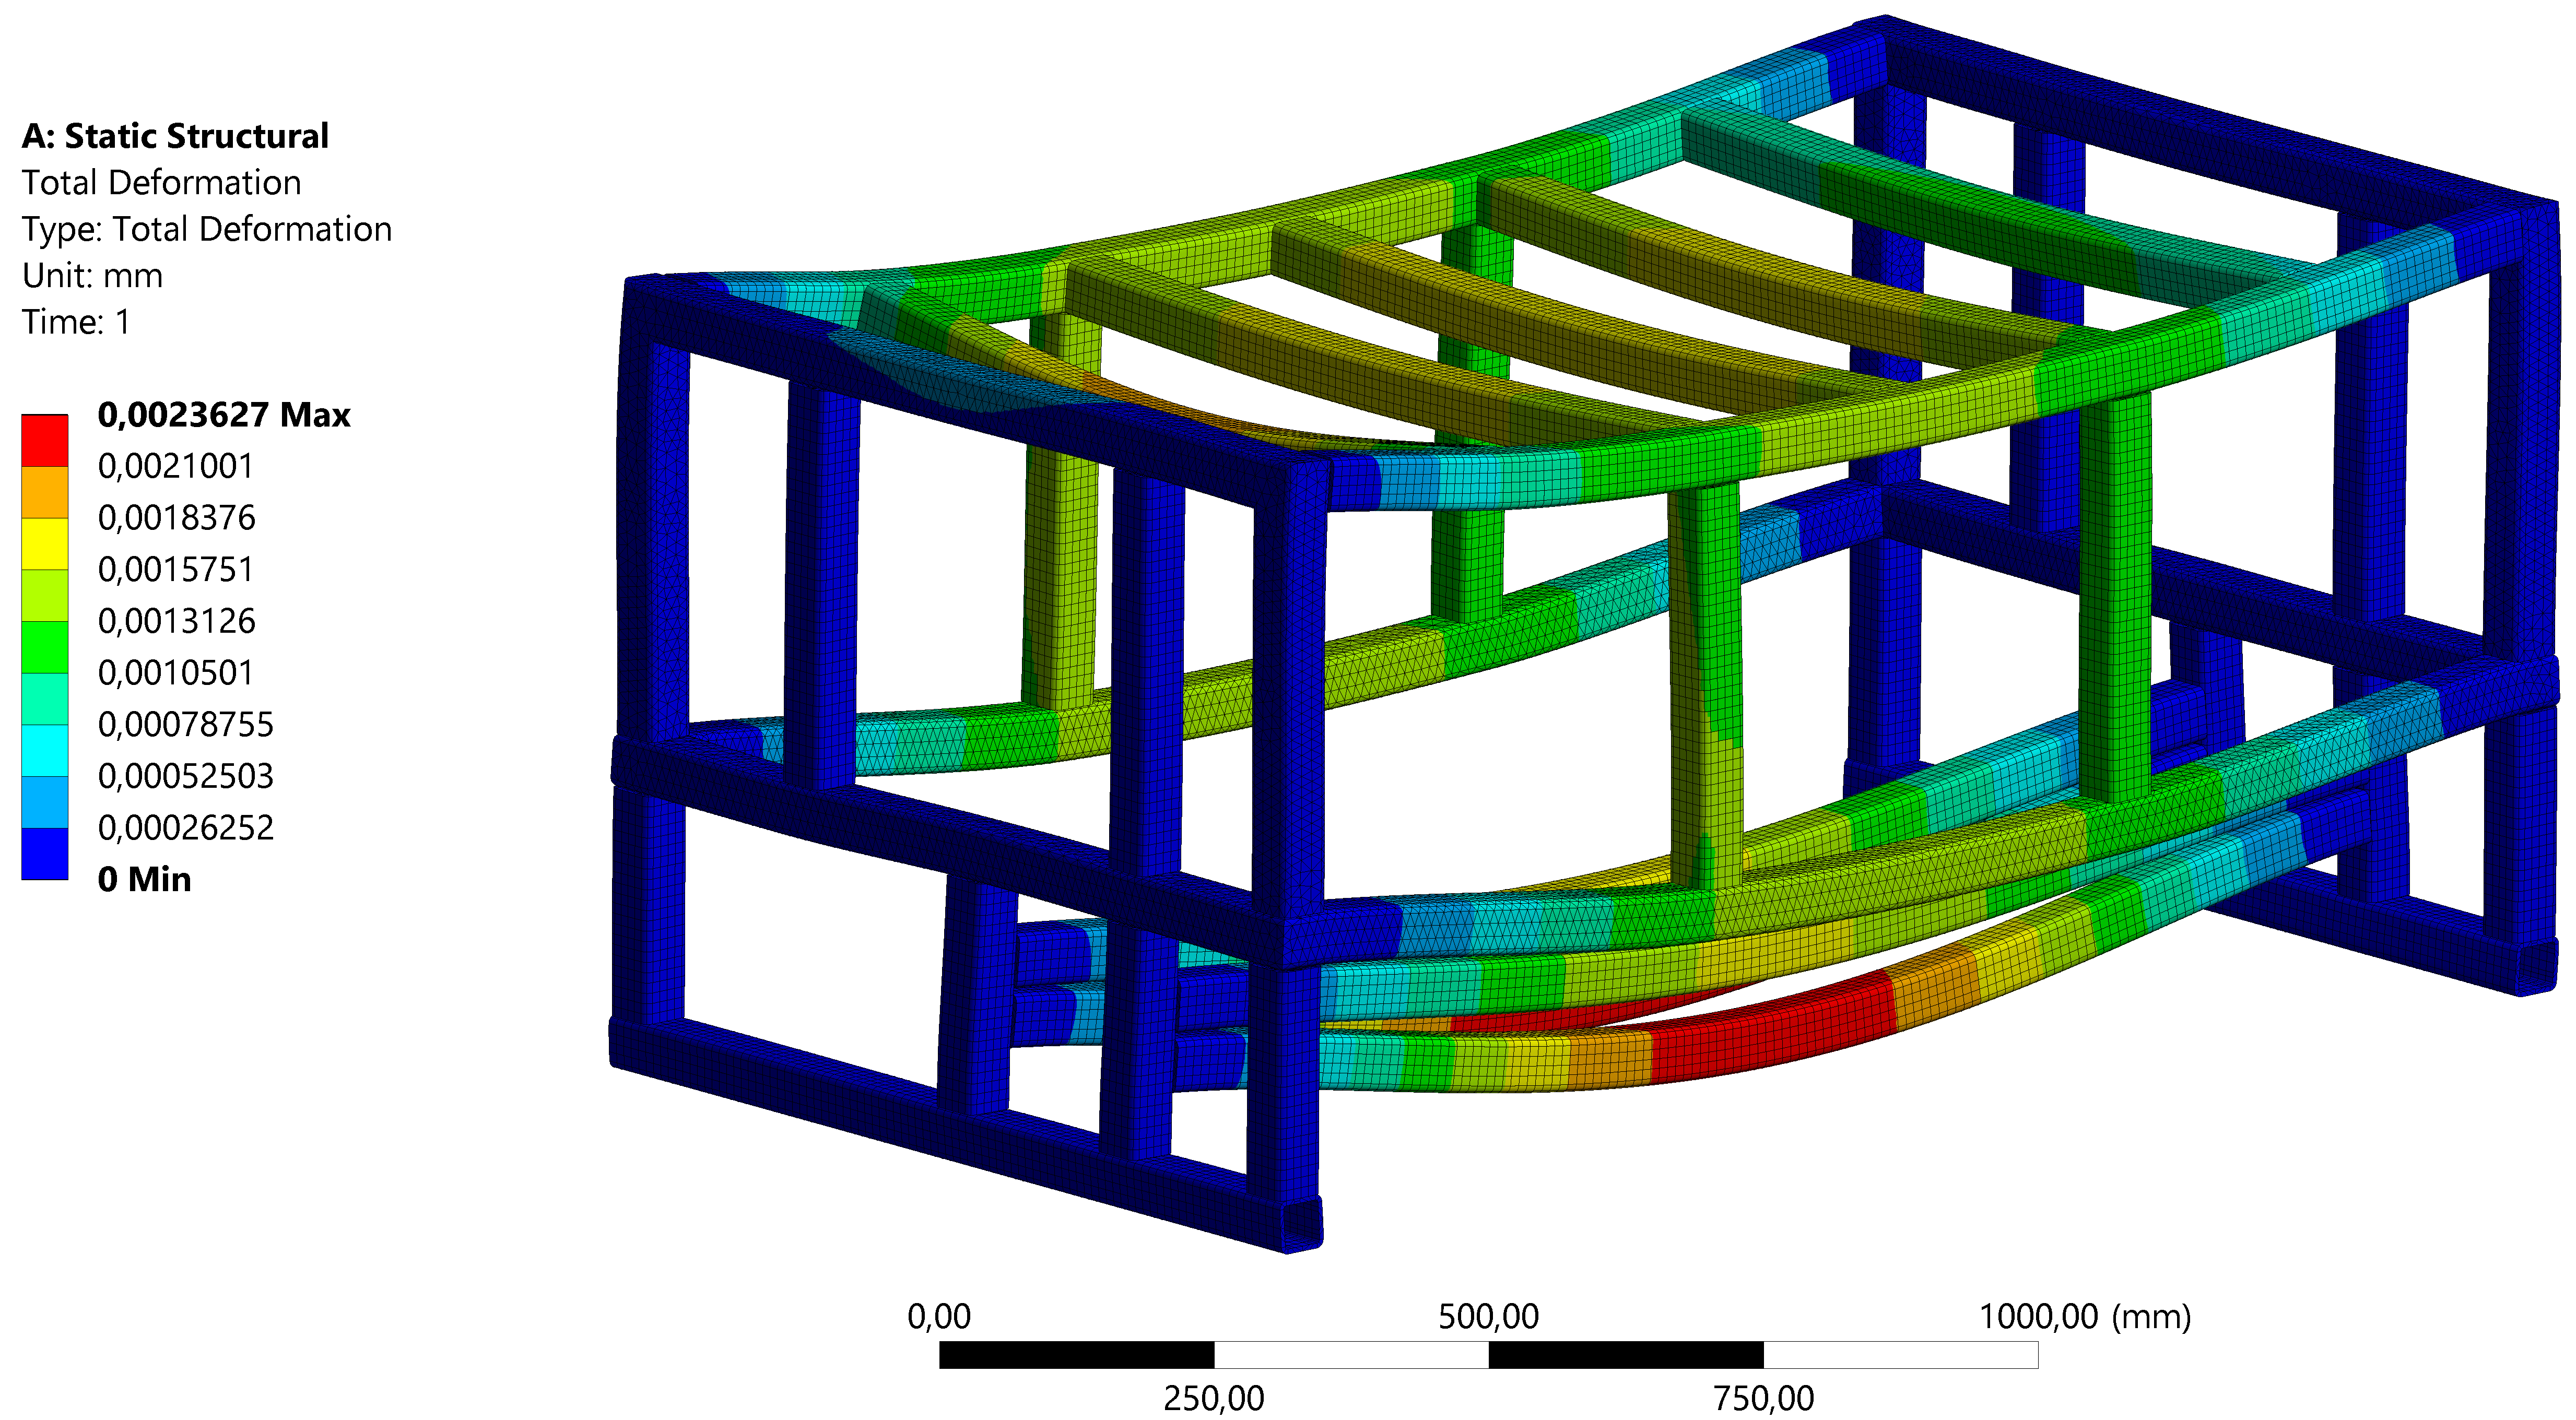
\includegraphics[width=1\textwidth]{figuras/estrutura/AnaliseEstaticaTubular/Deformation_Tubular.png}
    \caption{Análise da deformação total da estrutura }
    \label{fig:deformation_tubular}
\end{figure}

%\begin{figure}[ht]
%    \centering
%    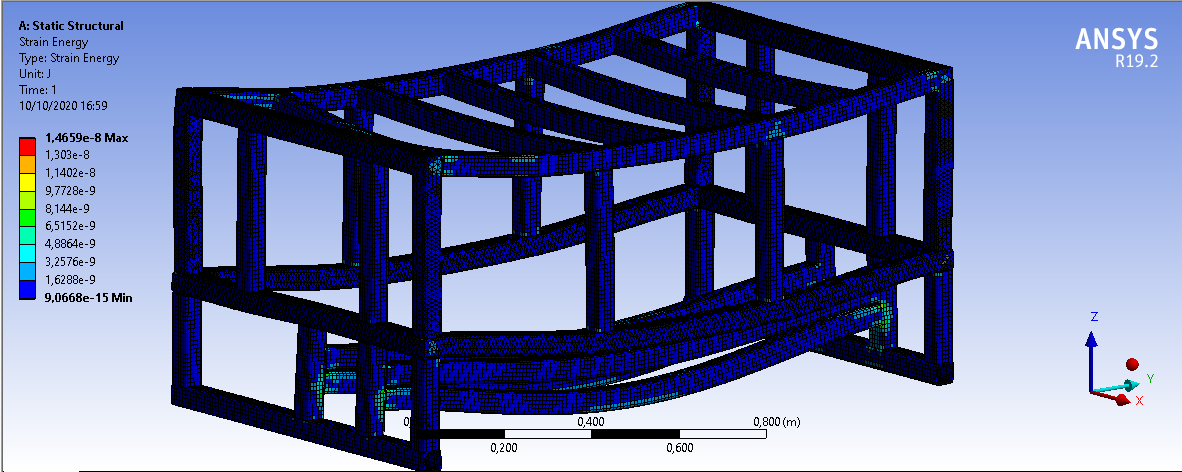
\includegraphics[width=1\textwidth]{figuras/estrutura/AnaliseEstaticaTubular/Energy_tubular.png}
%    \caption{Análise da Energia de tensão da estrutura}
%    \label{fig:Energy_Strain}
%\end{figure}

\begin{figure}[ht]
    \centering
    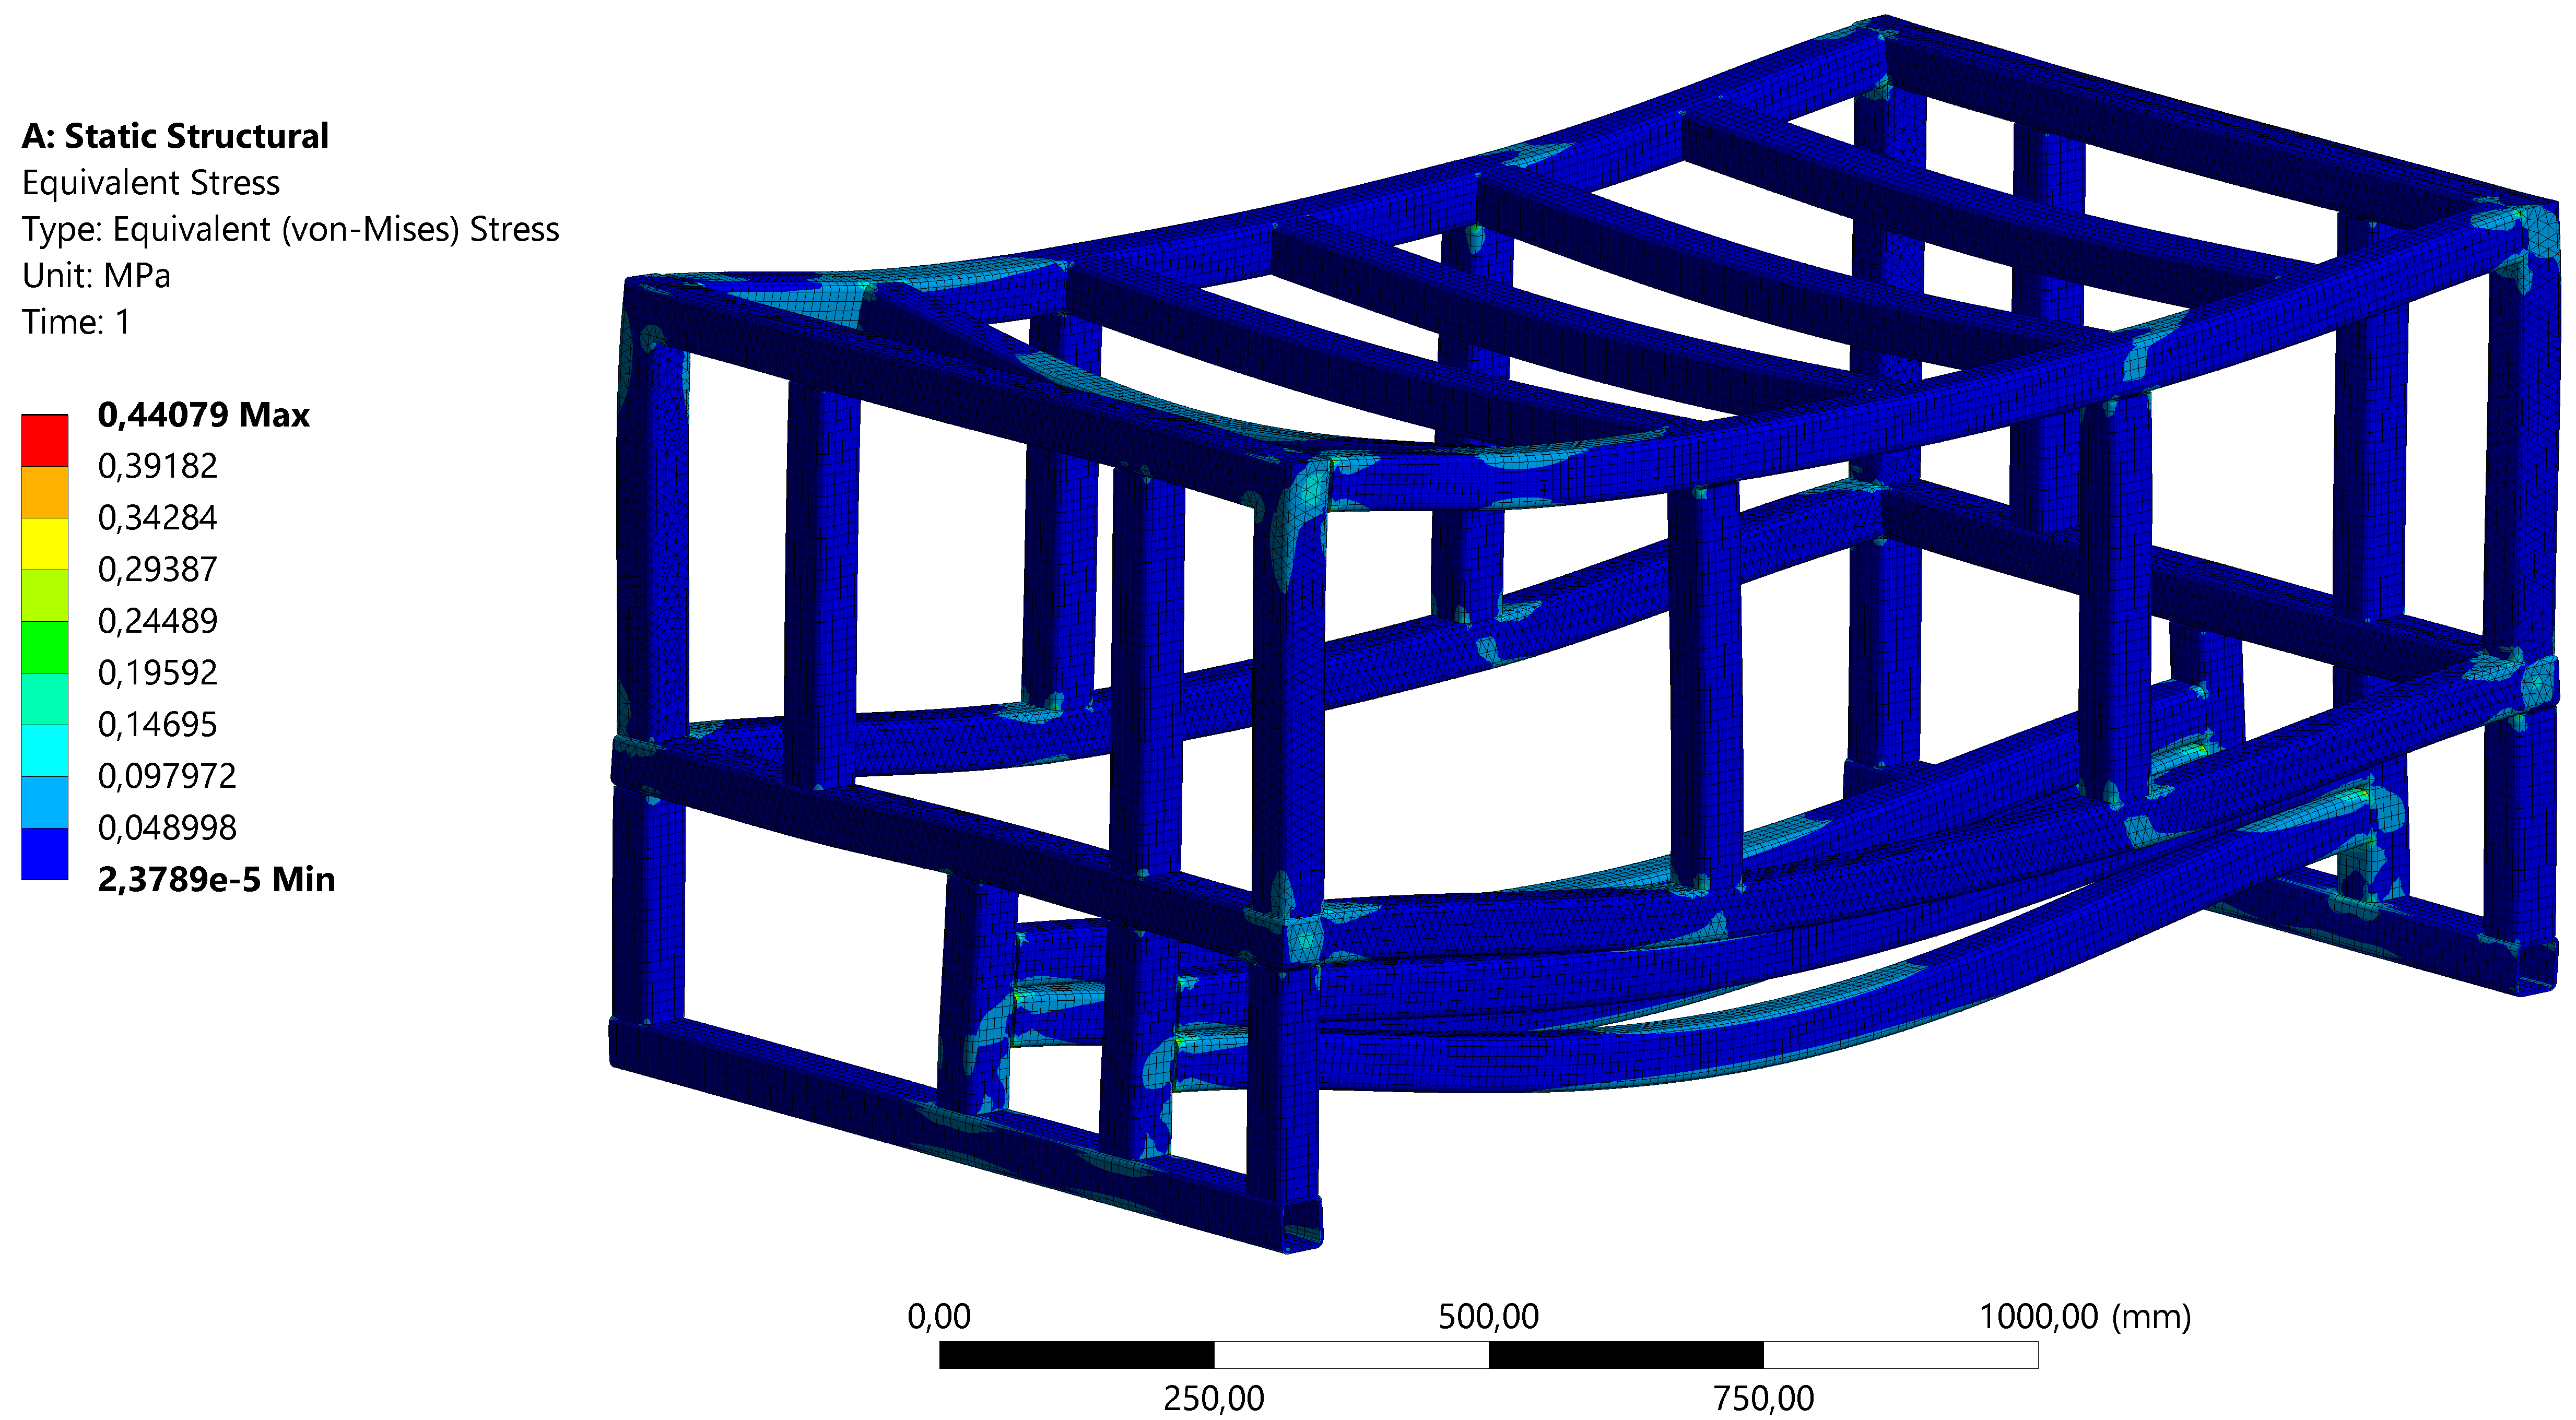
\includegraphics[width=1\textwidth]{figuras/estrutura/AnaliseEstaticaTubular/Von-Mises Stress_Tubular.png}
    \caption{Análise da Tensão Equivalente von Mises}
    \label{fig:Von_Mises_tubular}
\end{figure}

Pode-se concluir, pelas figuras supracitadas e valores máximos apresentados, que a estrutura comporta facilmente todas as cargas aplicadas e devido aos baixos valores apresentados, viu-se a oportunidade de trazer aspectos ergonômicos para o produto alterando-se a altura da estrutura por meio de tubos de apoio, que por conta de serem estrategicamente posicionados, não se esperam mudanças significativas a ponto de se fazer necessárias outras avaliações por simulação.


\subsection{Análise de Vibrações} \label{section:AnaliseVibracoes}
A proposta apresentada para vibrações compreende um estudo limitado ao conhecimento das frequências naturais do objeto em estudo e validações somente para aspecto estacionário de operação do motor, o qual é bem estabelecido teoricamente e se dará principalmente ao fato da ausência de mecanismos para análise experimental do protótipo, afim de caracterizar efeitos transientes, coeficientes de armotecimento e elátisco do componente estrutural, e portanto conhecimento apenas dos graus de liberdade de vibração da estrutura.

A abordagem então faz uso do método teórico conhecido como análise modal, o qual representa o comportamento físico de vibração de componentes estruturais acoplados para uma transformação na qual esse fenômeno é convertido em um sistema de múltiplos graus de liberdade desacoplados \cite{inmanbook}, fornecidos através de frequências naturais, formas modais e, adicionalmente, fatores de participação modal em uma estrutura.

Na abordagem realizada pela análise modal, a vibração máxima ocorre nas frequências naturais ou harmônicas, e geralmente se deve evitar. Em outras palavras, o estudo dos graus de liberdade da estrutura nos diz em quais frequências o sistema é vulnerável à vibrações com amplitude acentuadamente maior em consequência de um estímulo externo, ou em outras palavras, quando o sistema está exposto à ressonância \cite{inmanbook}. Justifica-se o tópico em razão de que caso fossem descobertas frequências naturais dentro da faixa de excitação aplicada no equipamento, o projeto da estrutura teria que passar por mudanças afim de transladar as frequências naturais para fora da zona de excitação em que o produto iria operar.

Portanto, a forma dos modos produzidos pela análise modal nos diz como a estrutura tende a se deformar em razão de frequências naturais específicas e quais regiões sofreriam por concentradores de tensão e com isso, pode-se traçar estratégias para evitar principalmente possíveis consequências às juntas soldadas, com o desgaste gerado \cite{failure} ou ao impacto oriundo de tensões residuais na estrutura e seu efeito na resistência à fadiga do componente \cite{fatigue}. Além disso, os fatores de participação de modo nos dizem quais modos seriam mais estimulados, que para interesse prático, têm valor significativo apenas para os 10 primeiros componentes modais \cite{inmanbook}.

Para condições de contorno, foram adotadas as configurações de corpo livre, situação na qual pode-se fazer análise das frêquencias naturais do subgrupos. Com relação aos contatos, devido à falta de fixação entre as engrenagens e o fuso no modelo simplificado, foi aderido a configuração \textit{bonded} ao invés do \textit{frictional} por se assemelhar mais ao comportamento real da estrutura.
As formas modais naturais são apresentadas nas Fig. \ref{fig:modos12}, \ref{fig:modos34}, \ref{fig:modos56}, \ref{fig:modos78} e \ref{fig:modos910}.

%Vale ressaltar que por conta dos seis graus de liberdade da estrutura na condição livre-livre levarão aos seis primeiros modos do corpo de prova a valor, pois tais modos representam os modos de corpo rígido, que são fisicamente consequência dos movimentos não restringidos do objeto \cite{inmanbook}. 
\begin{figure}[H]
\centering
\subfloat[Modo 1]{\label{fig:modo1}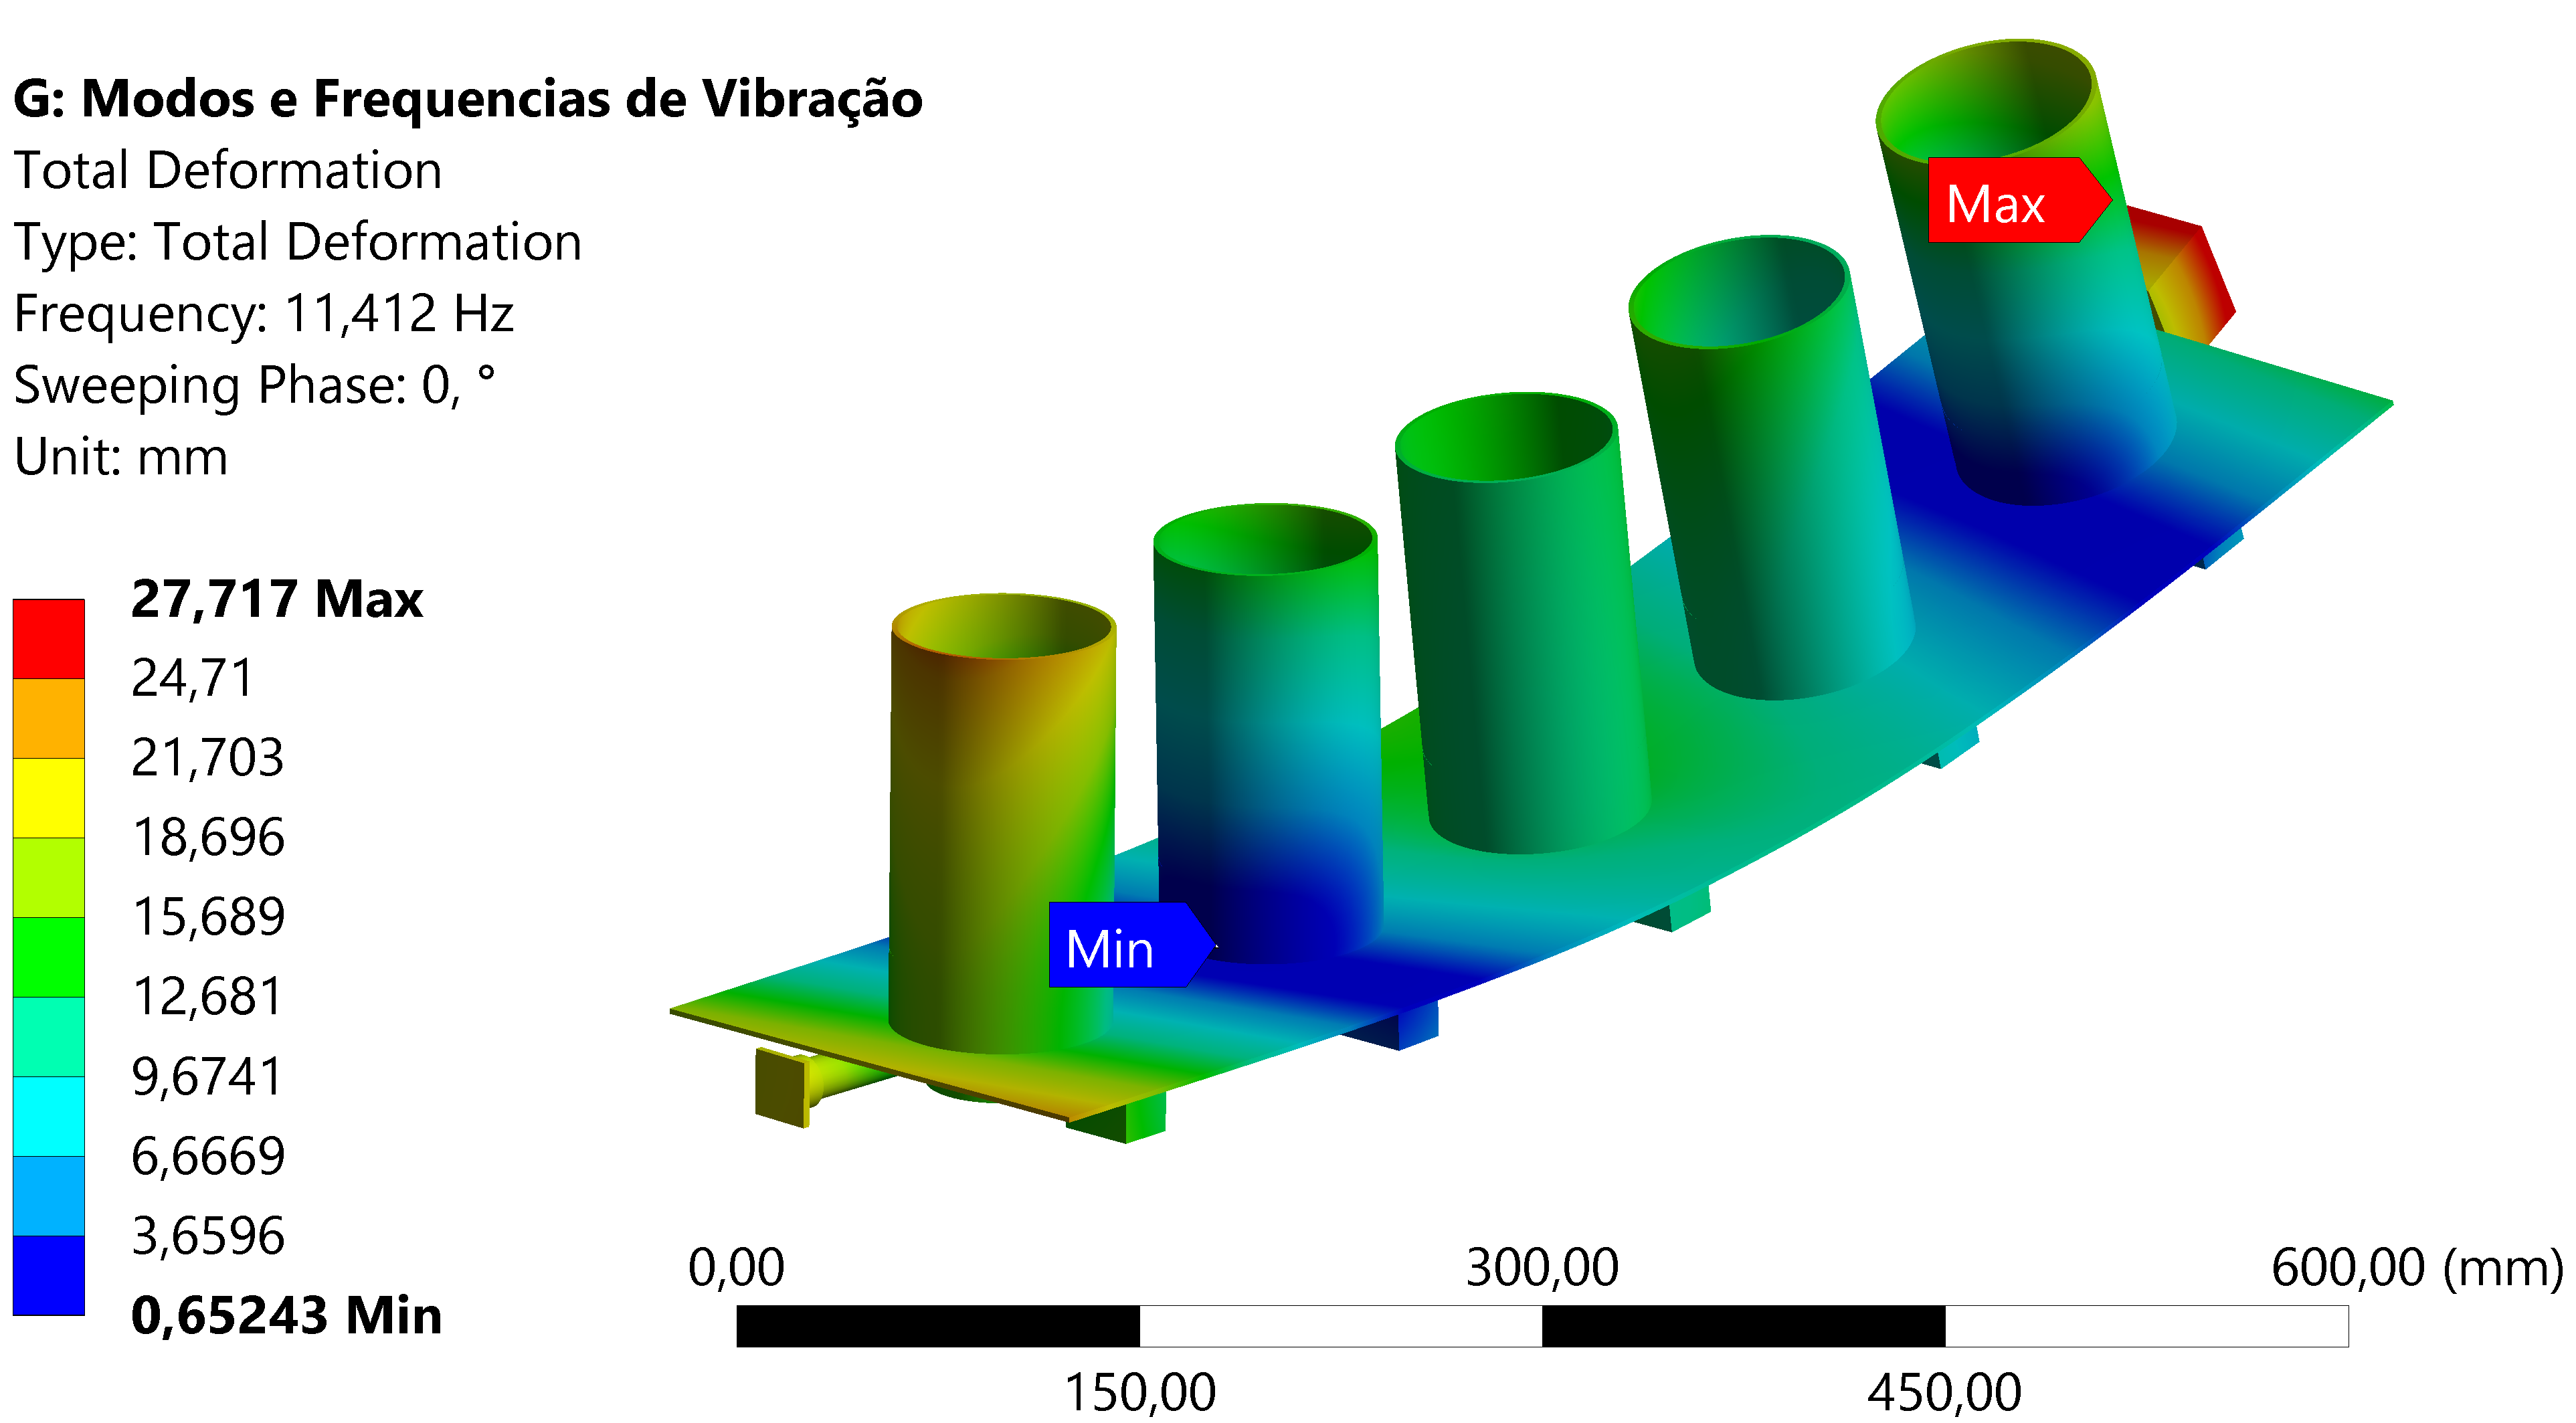
\includegraphics[width=.5\linewidth]{figuras/estrutura/Imagens PC3/Vibrações/modo 1.png}}\hfill
\subfloat[Modo 2]{\label{fig:modo2}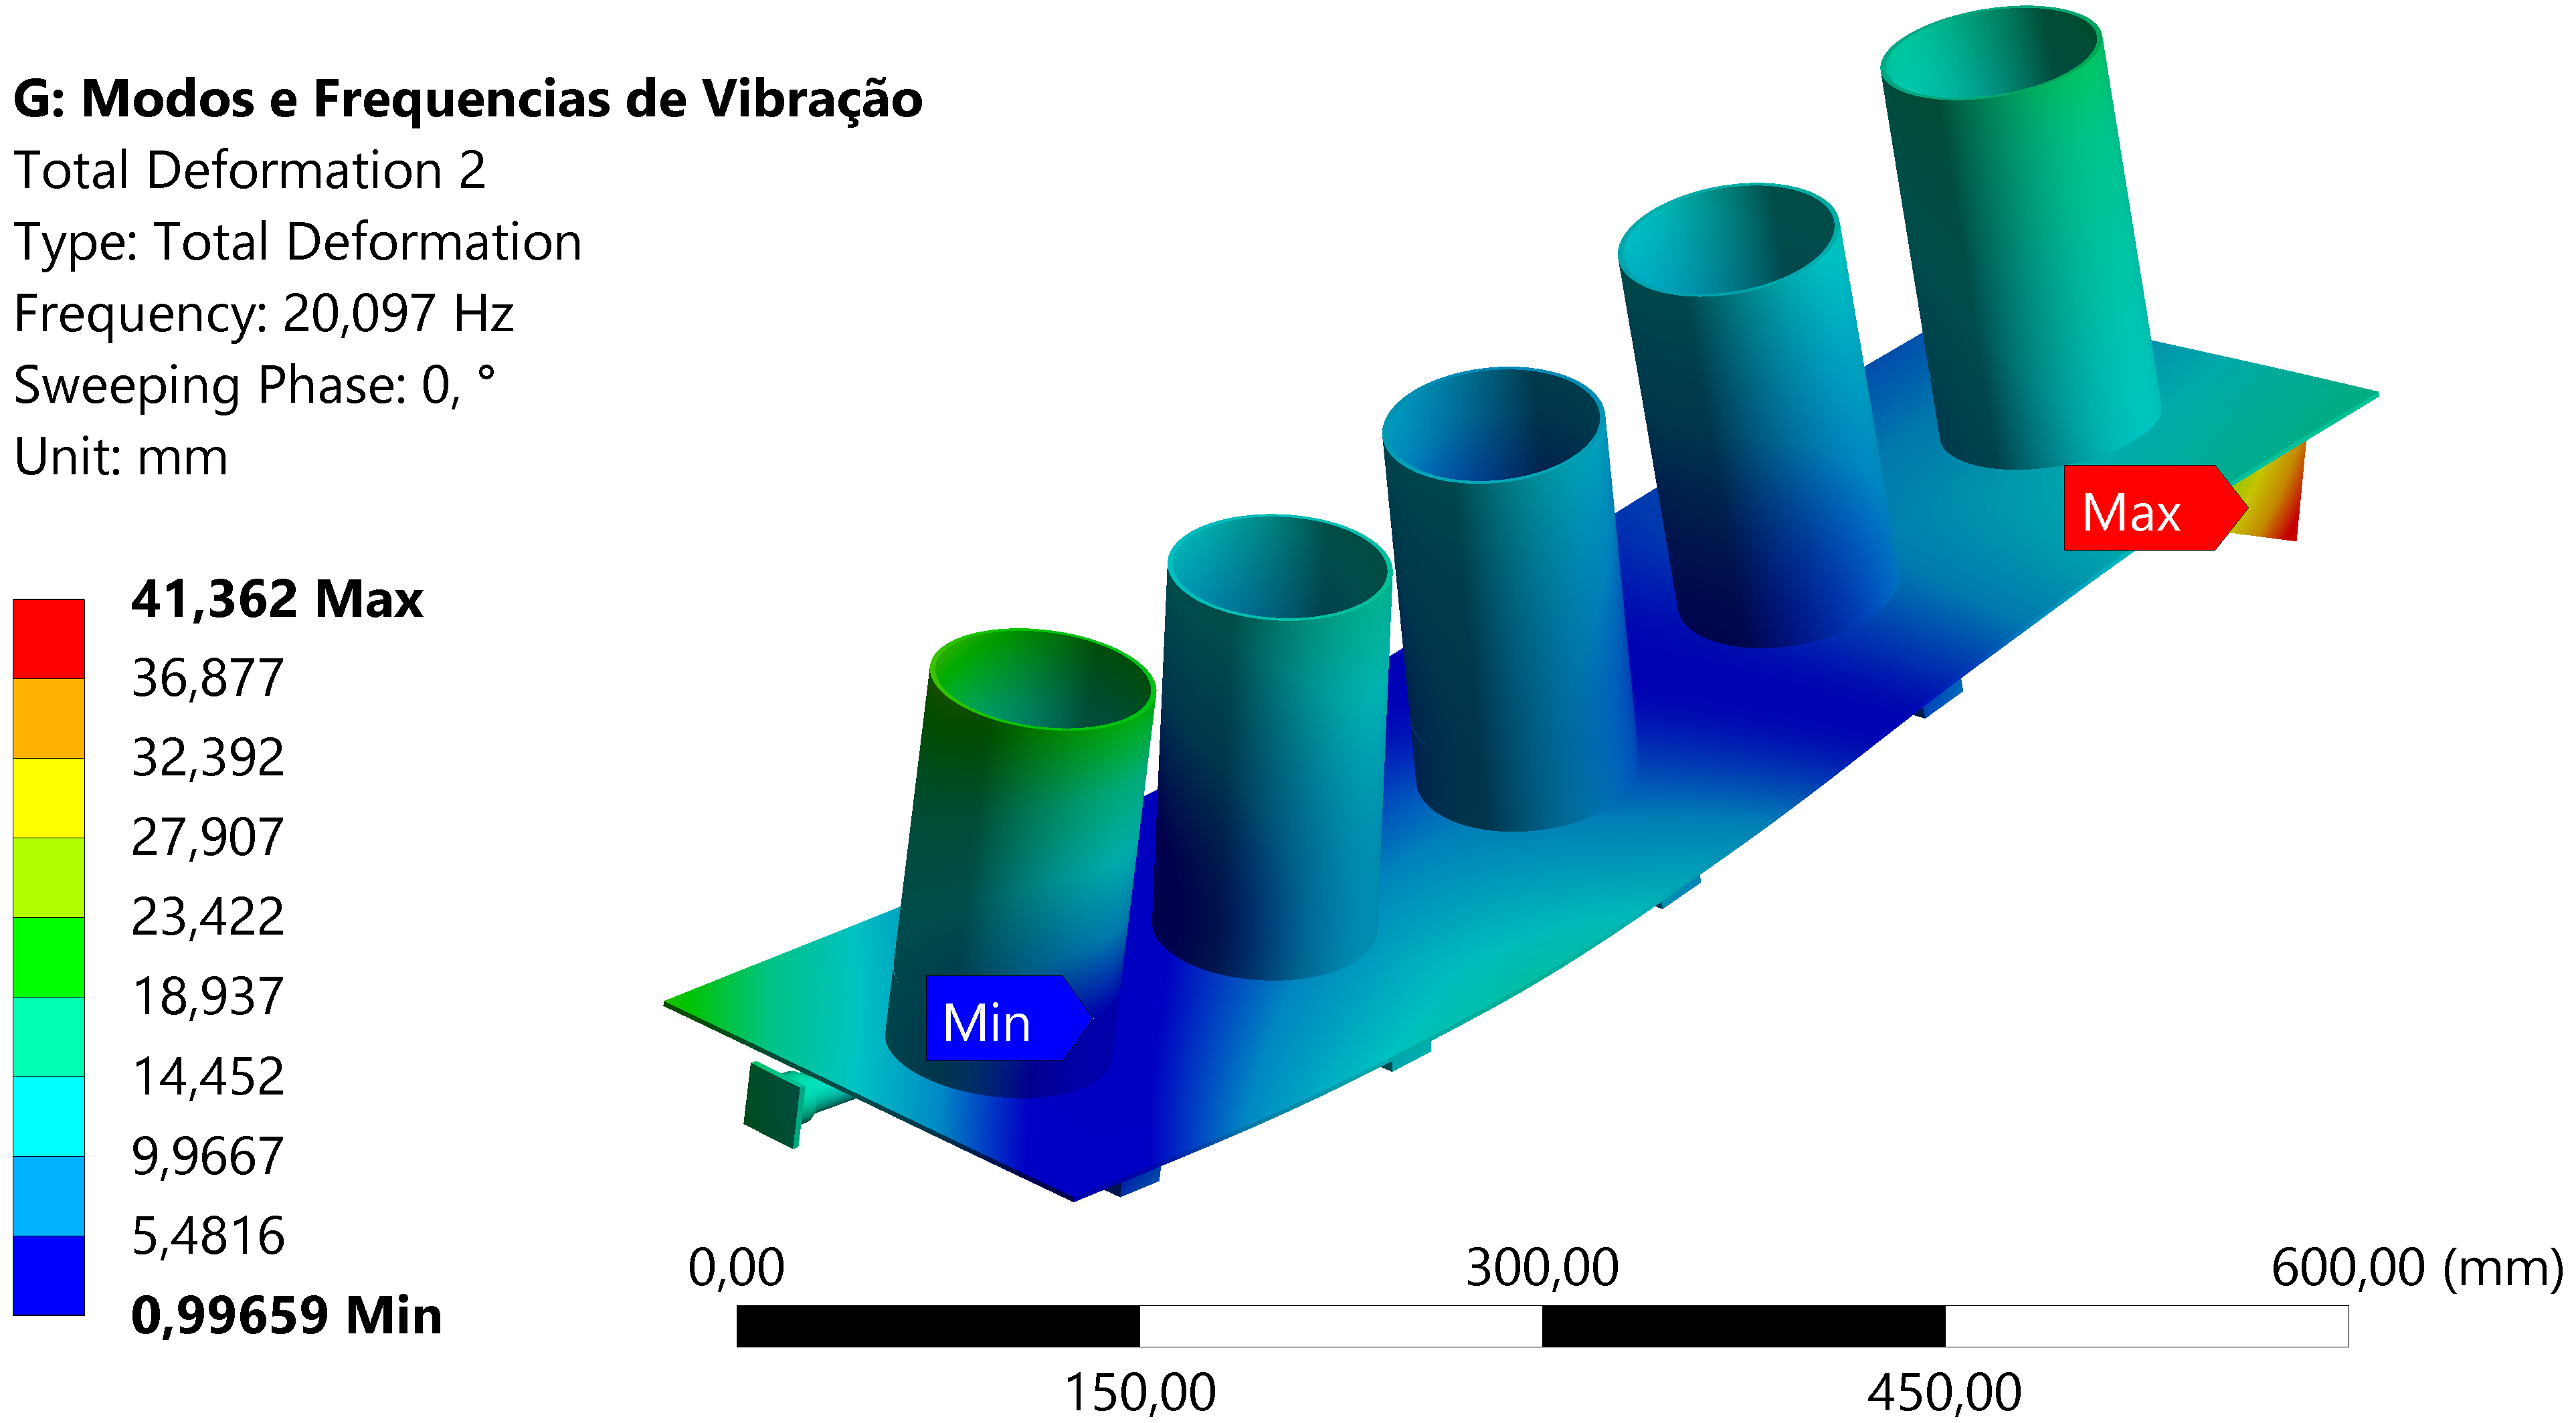
\includegraphics[width=.5\linewidth]{figuras/estrutura/Imagens PC3/Vibrações/modo 2.png}}\par 
\caption{Representação das formas modais 1 e 2}
\label{fig:modos12}
\end{figure}

\begin{figure}[H]
\centering
\subfloat[Modo 3]{\label{fig:modo3}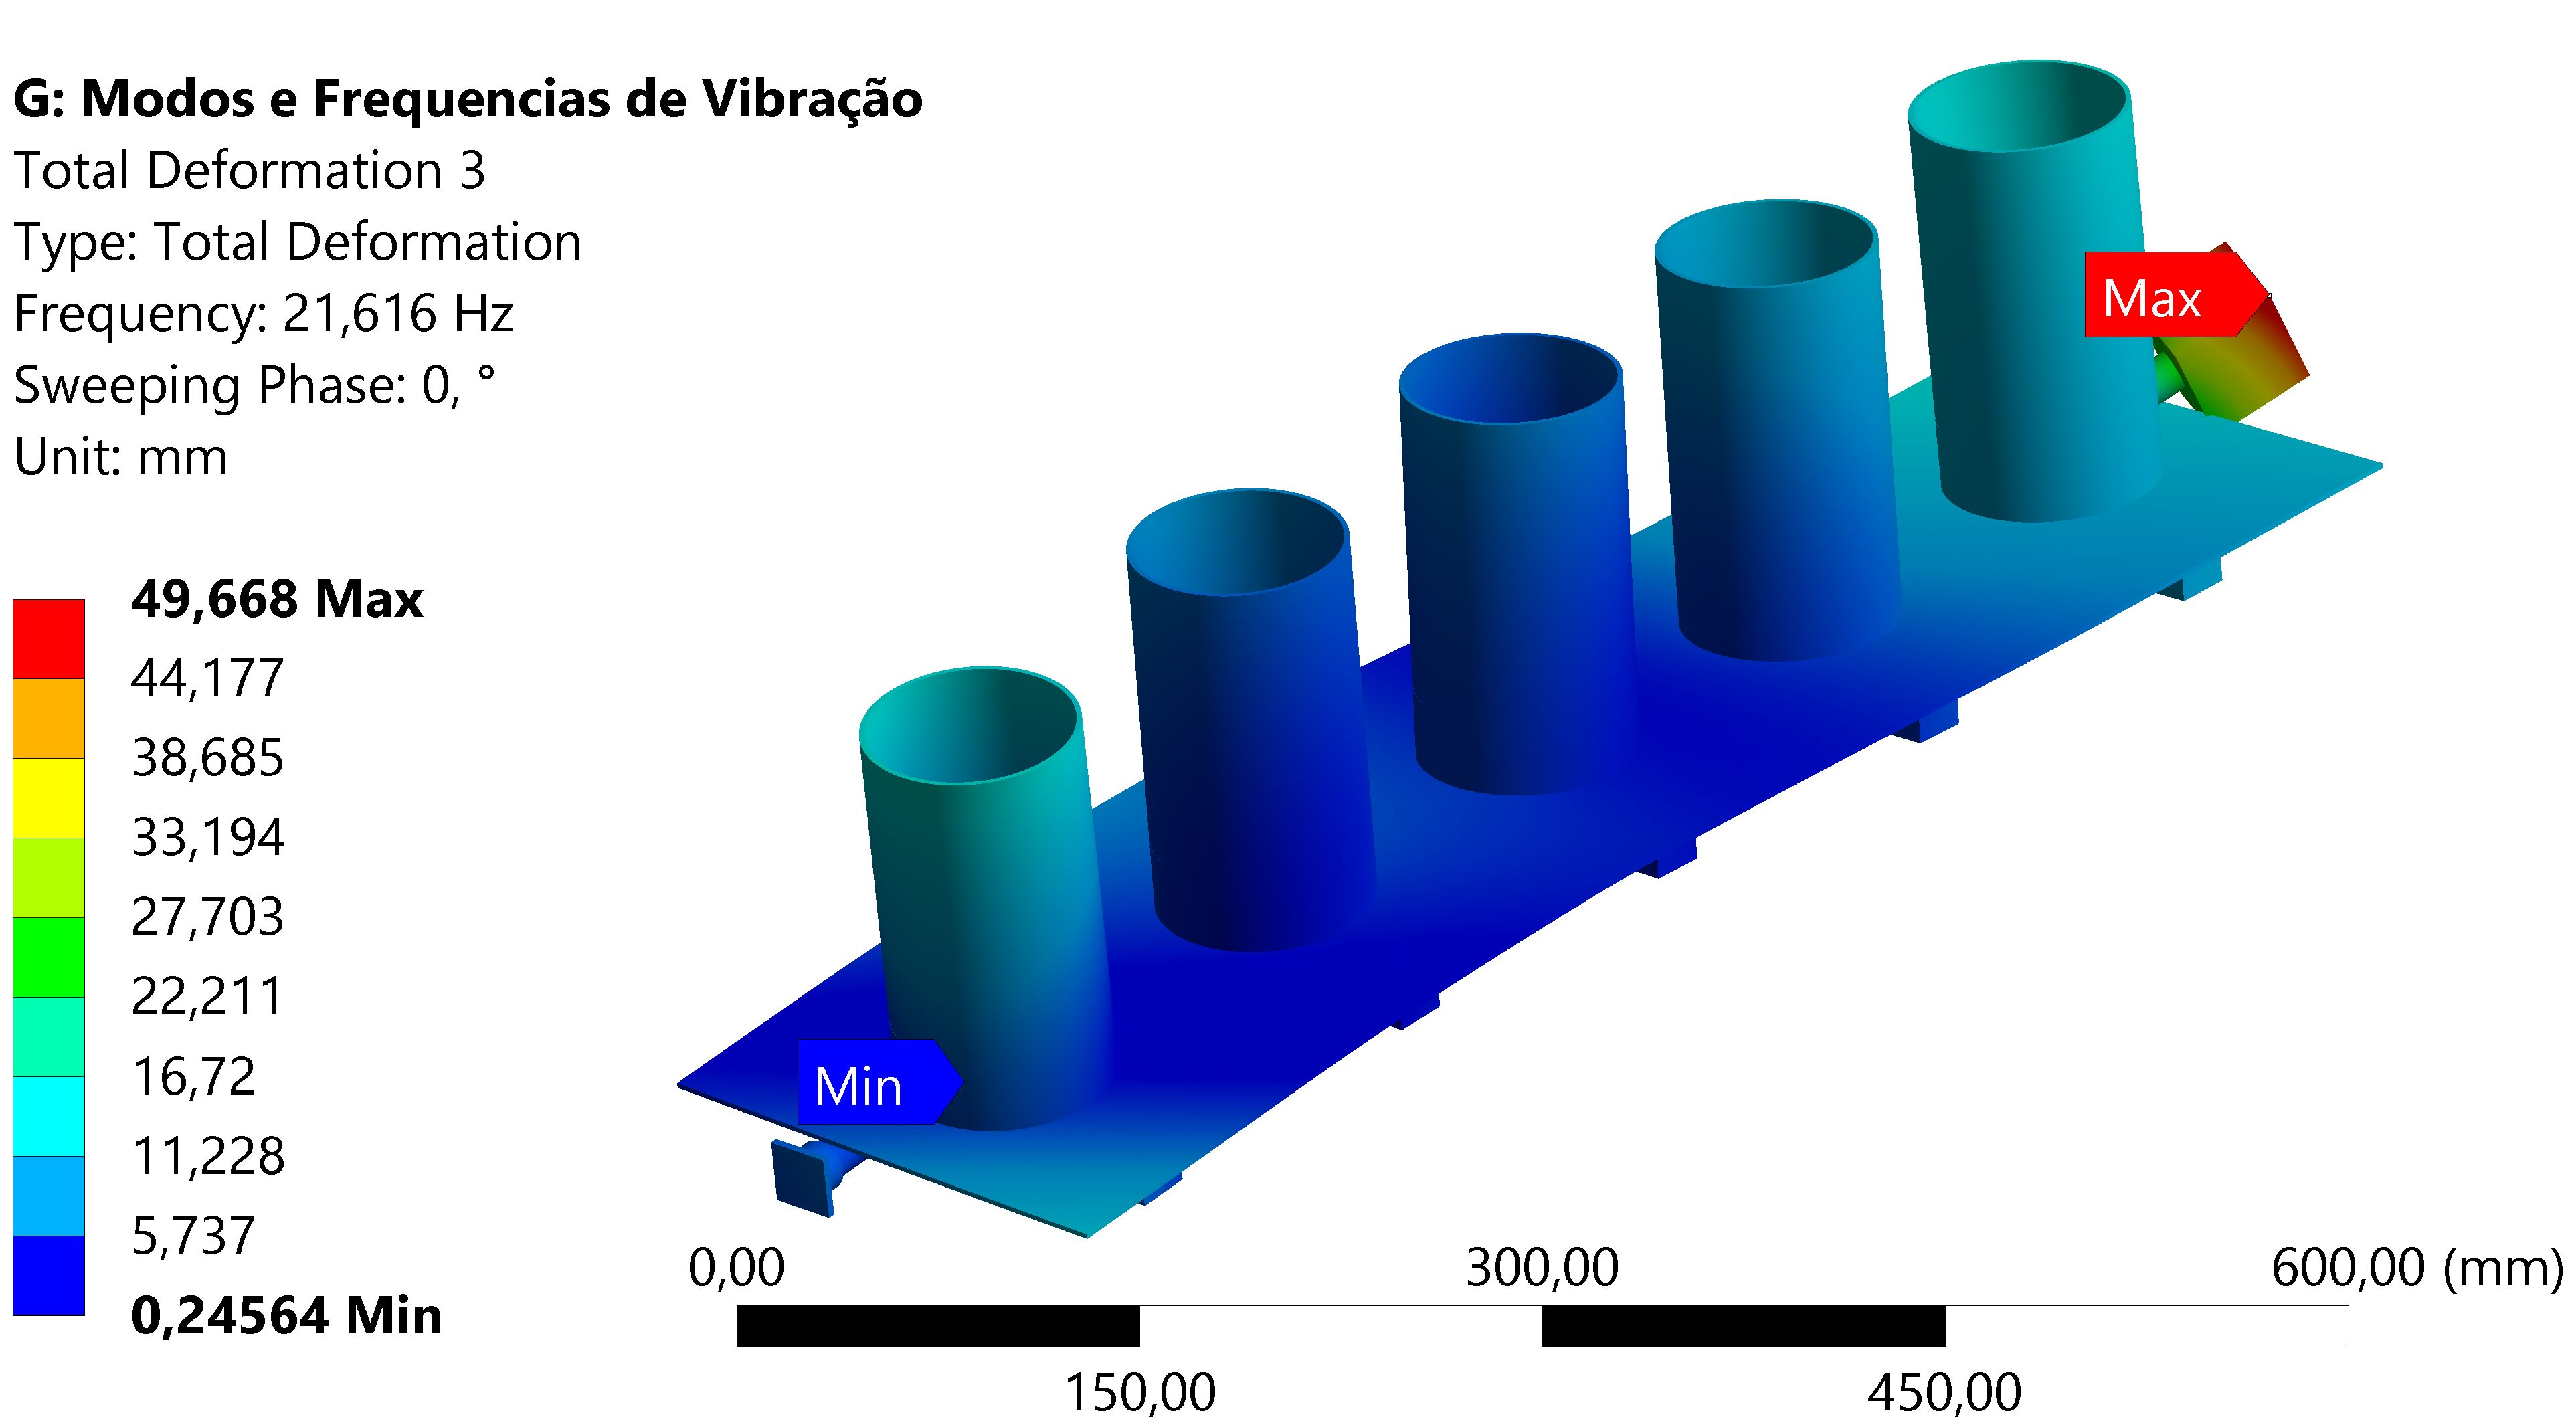
\includegraphics[width=.5\linewidth]{figuras/estrutura/Imagens PC3/Vibrações/modo 3.png}}\hfill
\subfloat[Modo 4]{\label{fig:modo4}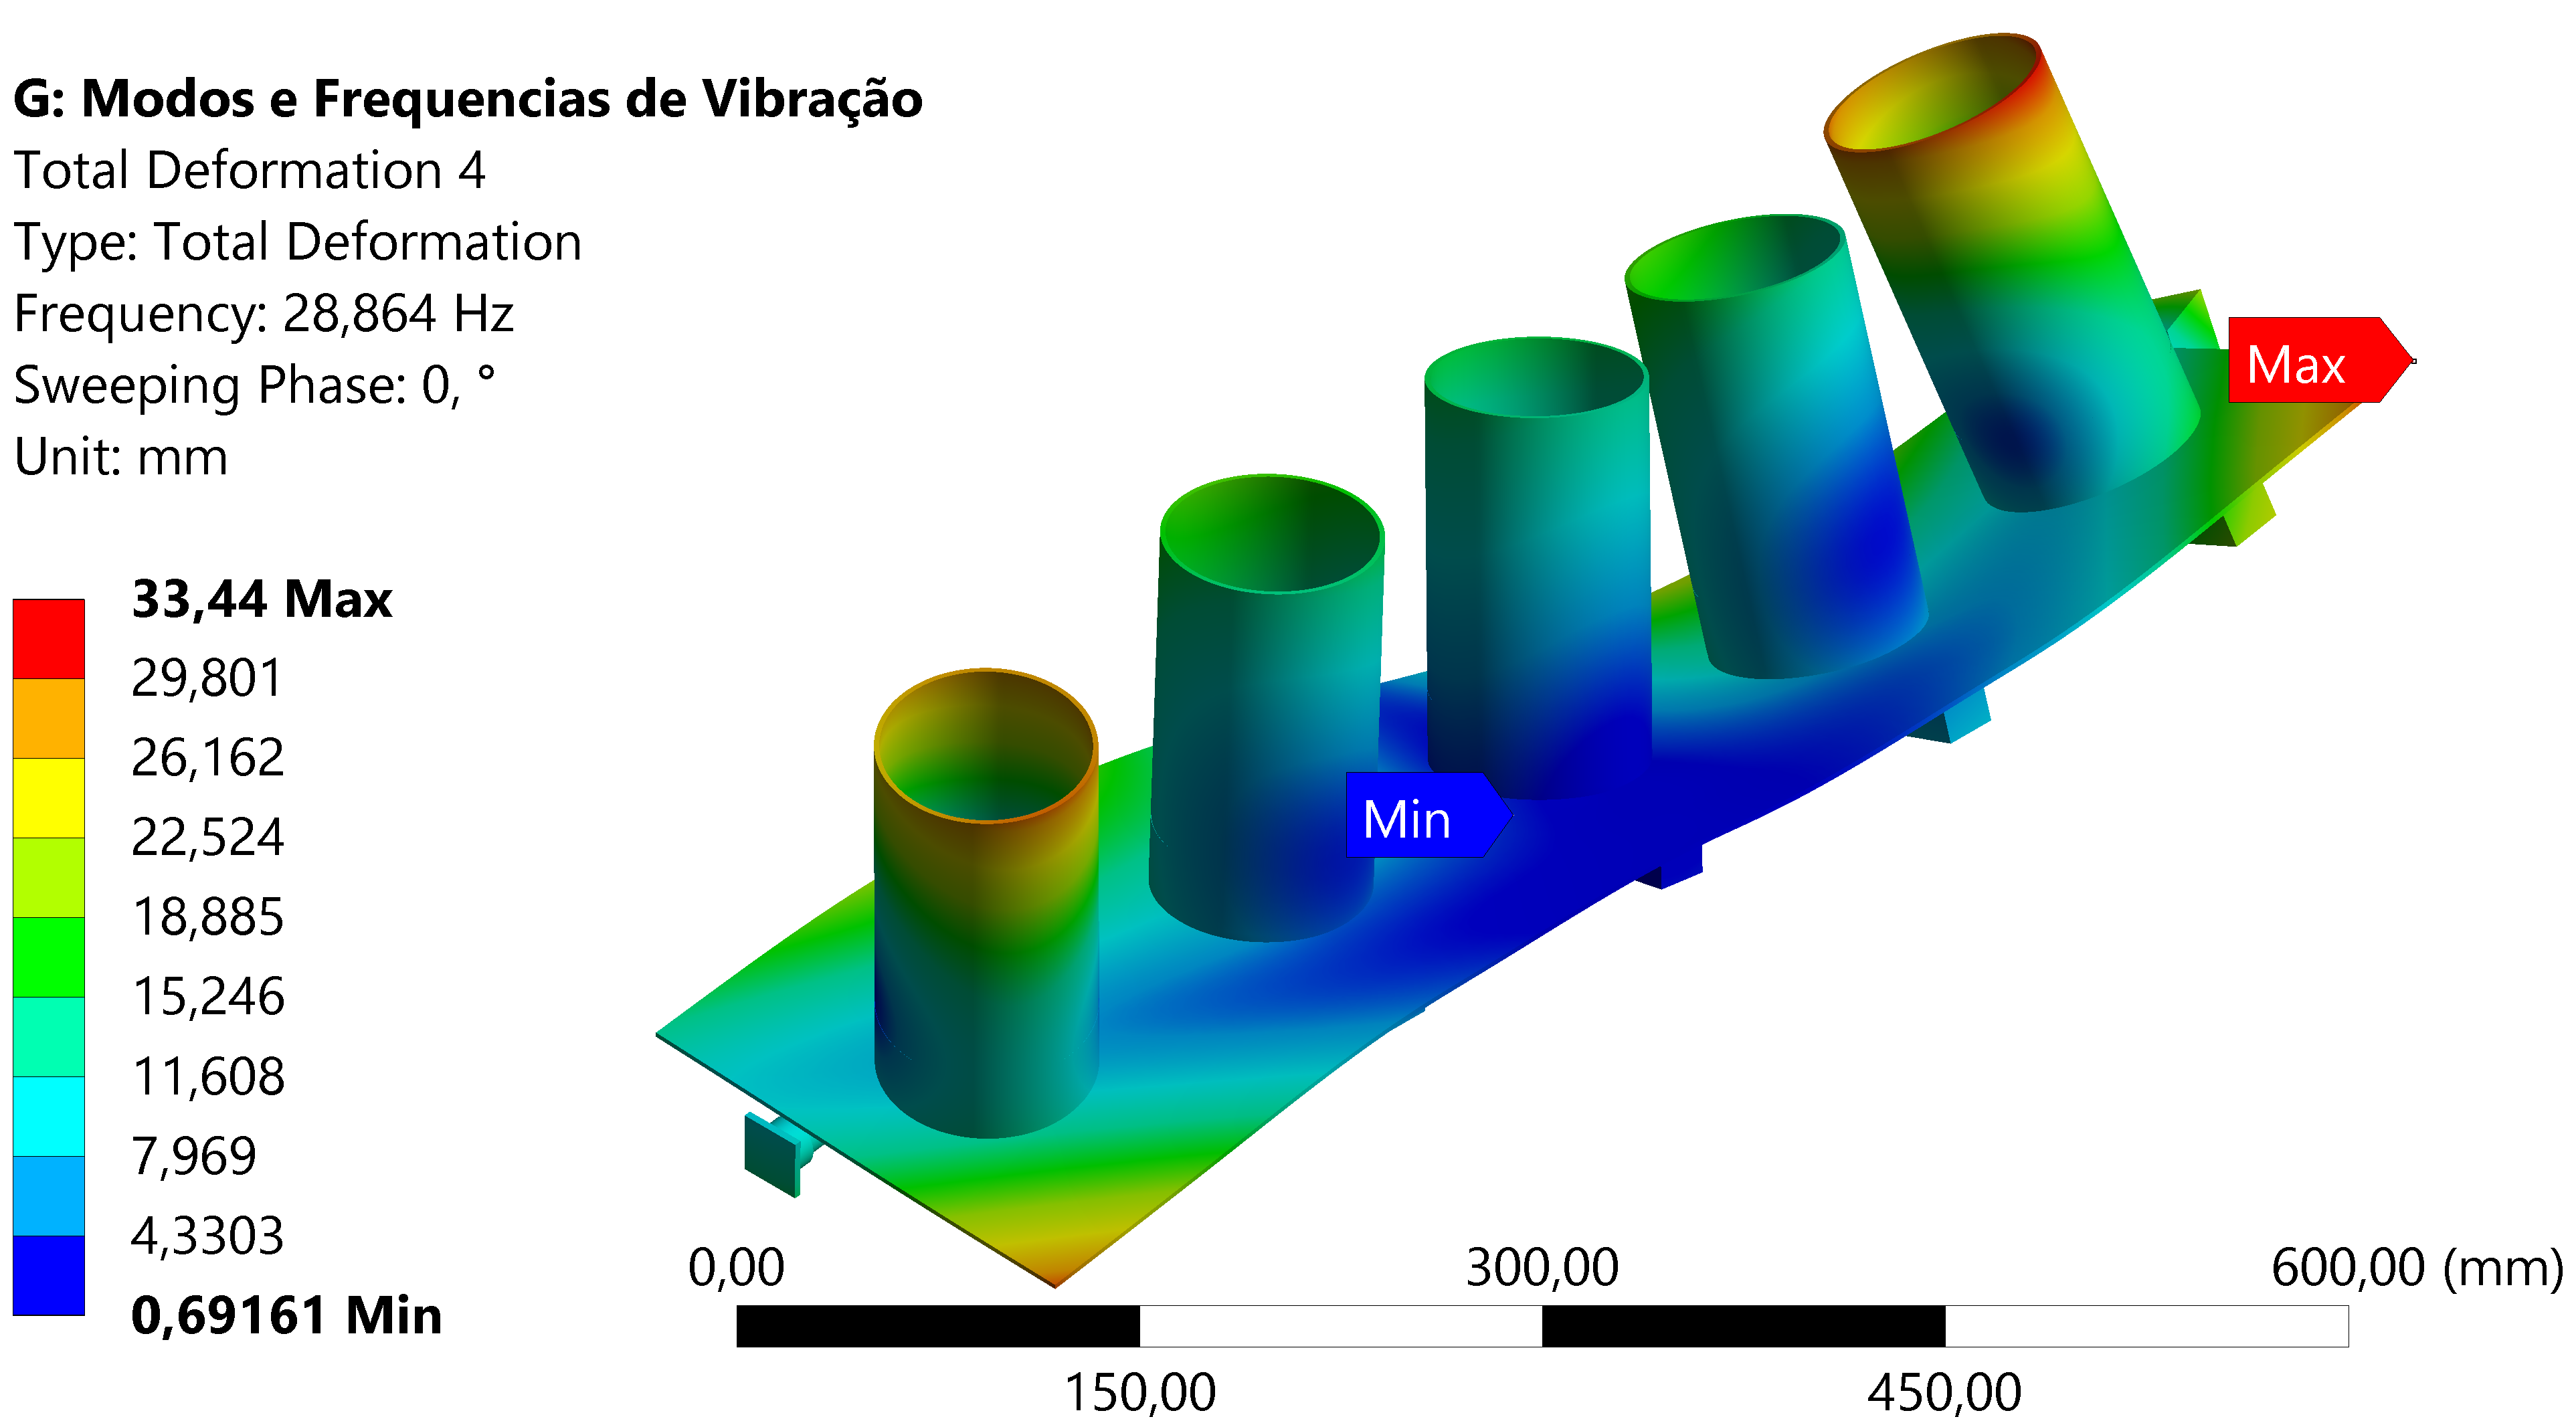
\includegraphics[width=.5\linewidth]{figuras/estrutura/Imagens PC3/Vibrações/modo 4.png}}\par 
\caption{Representação das formas modais 3 e 4}
\label{fig:modos34}
\end{figure}

\begin{figure}[H]
\centering
\subfloat[Modo 5]{\label{fig:modo5}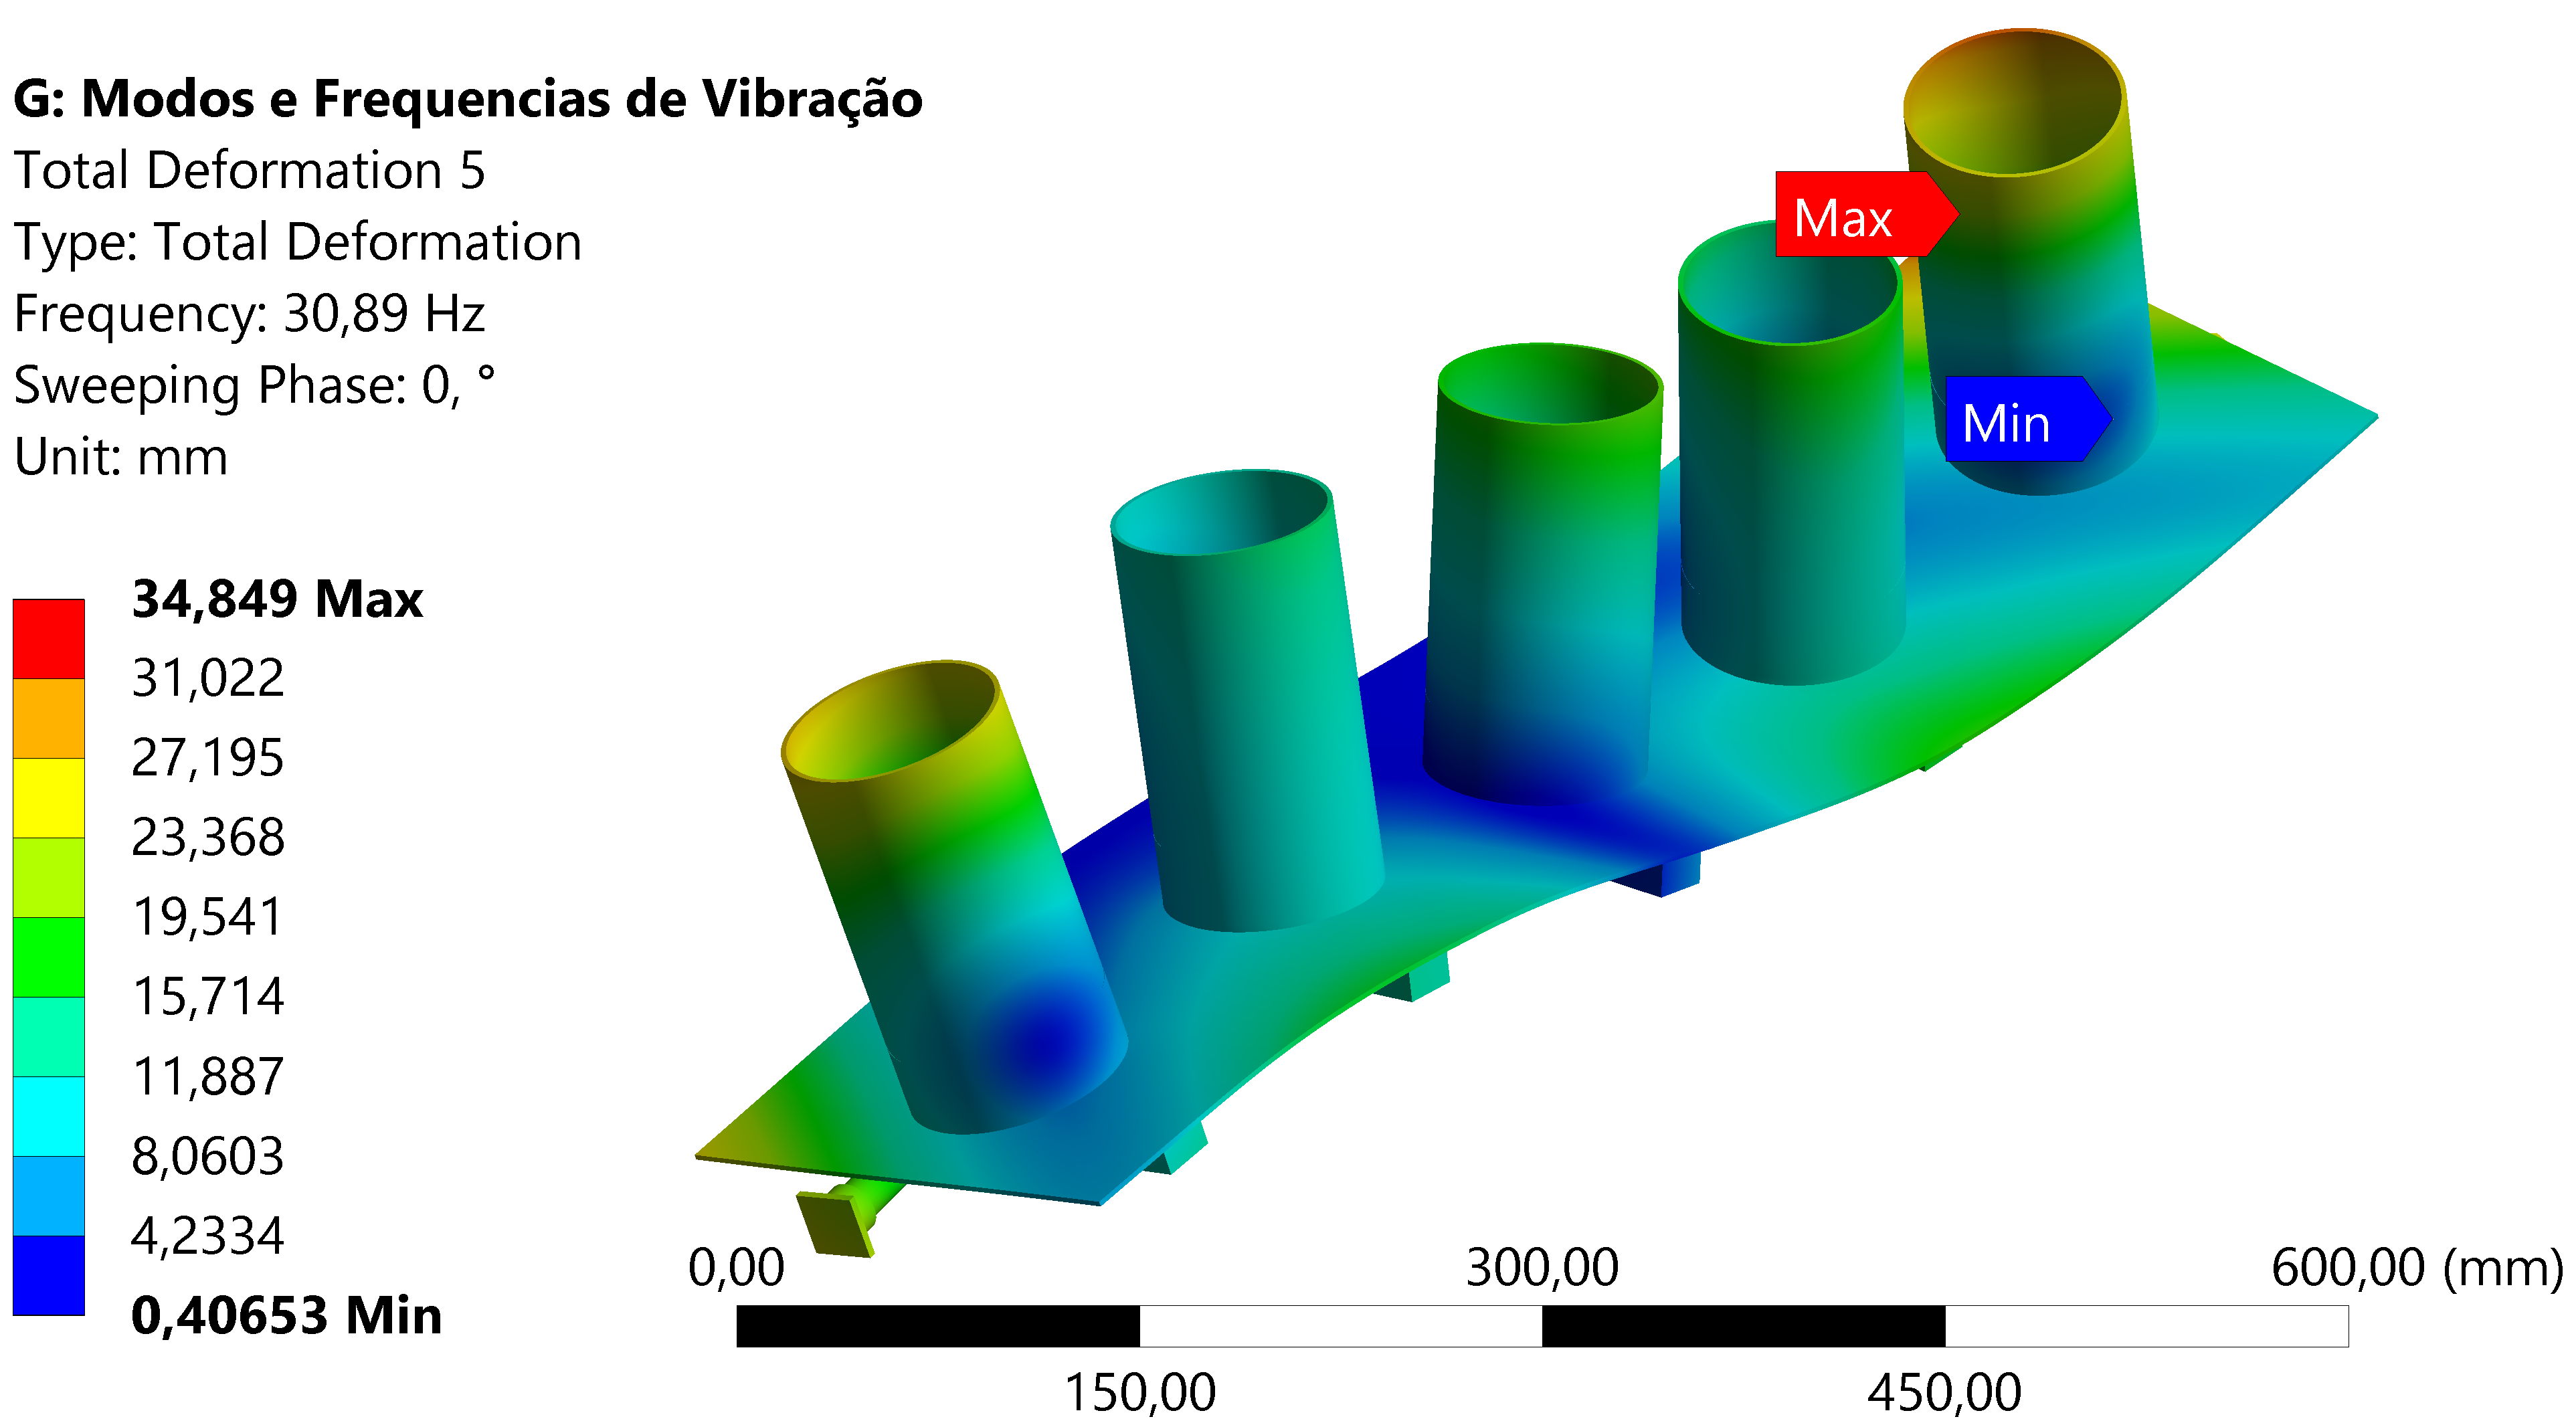
\includegraphics[width=.5\linewidth]{figuras/estrutura/Imagens PC3/Vibrações/modo 5.png}}\hfill
\subfloat[Modo 6]{\label{fig:modo6}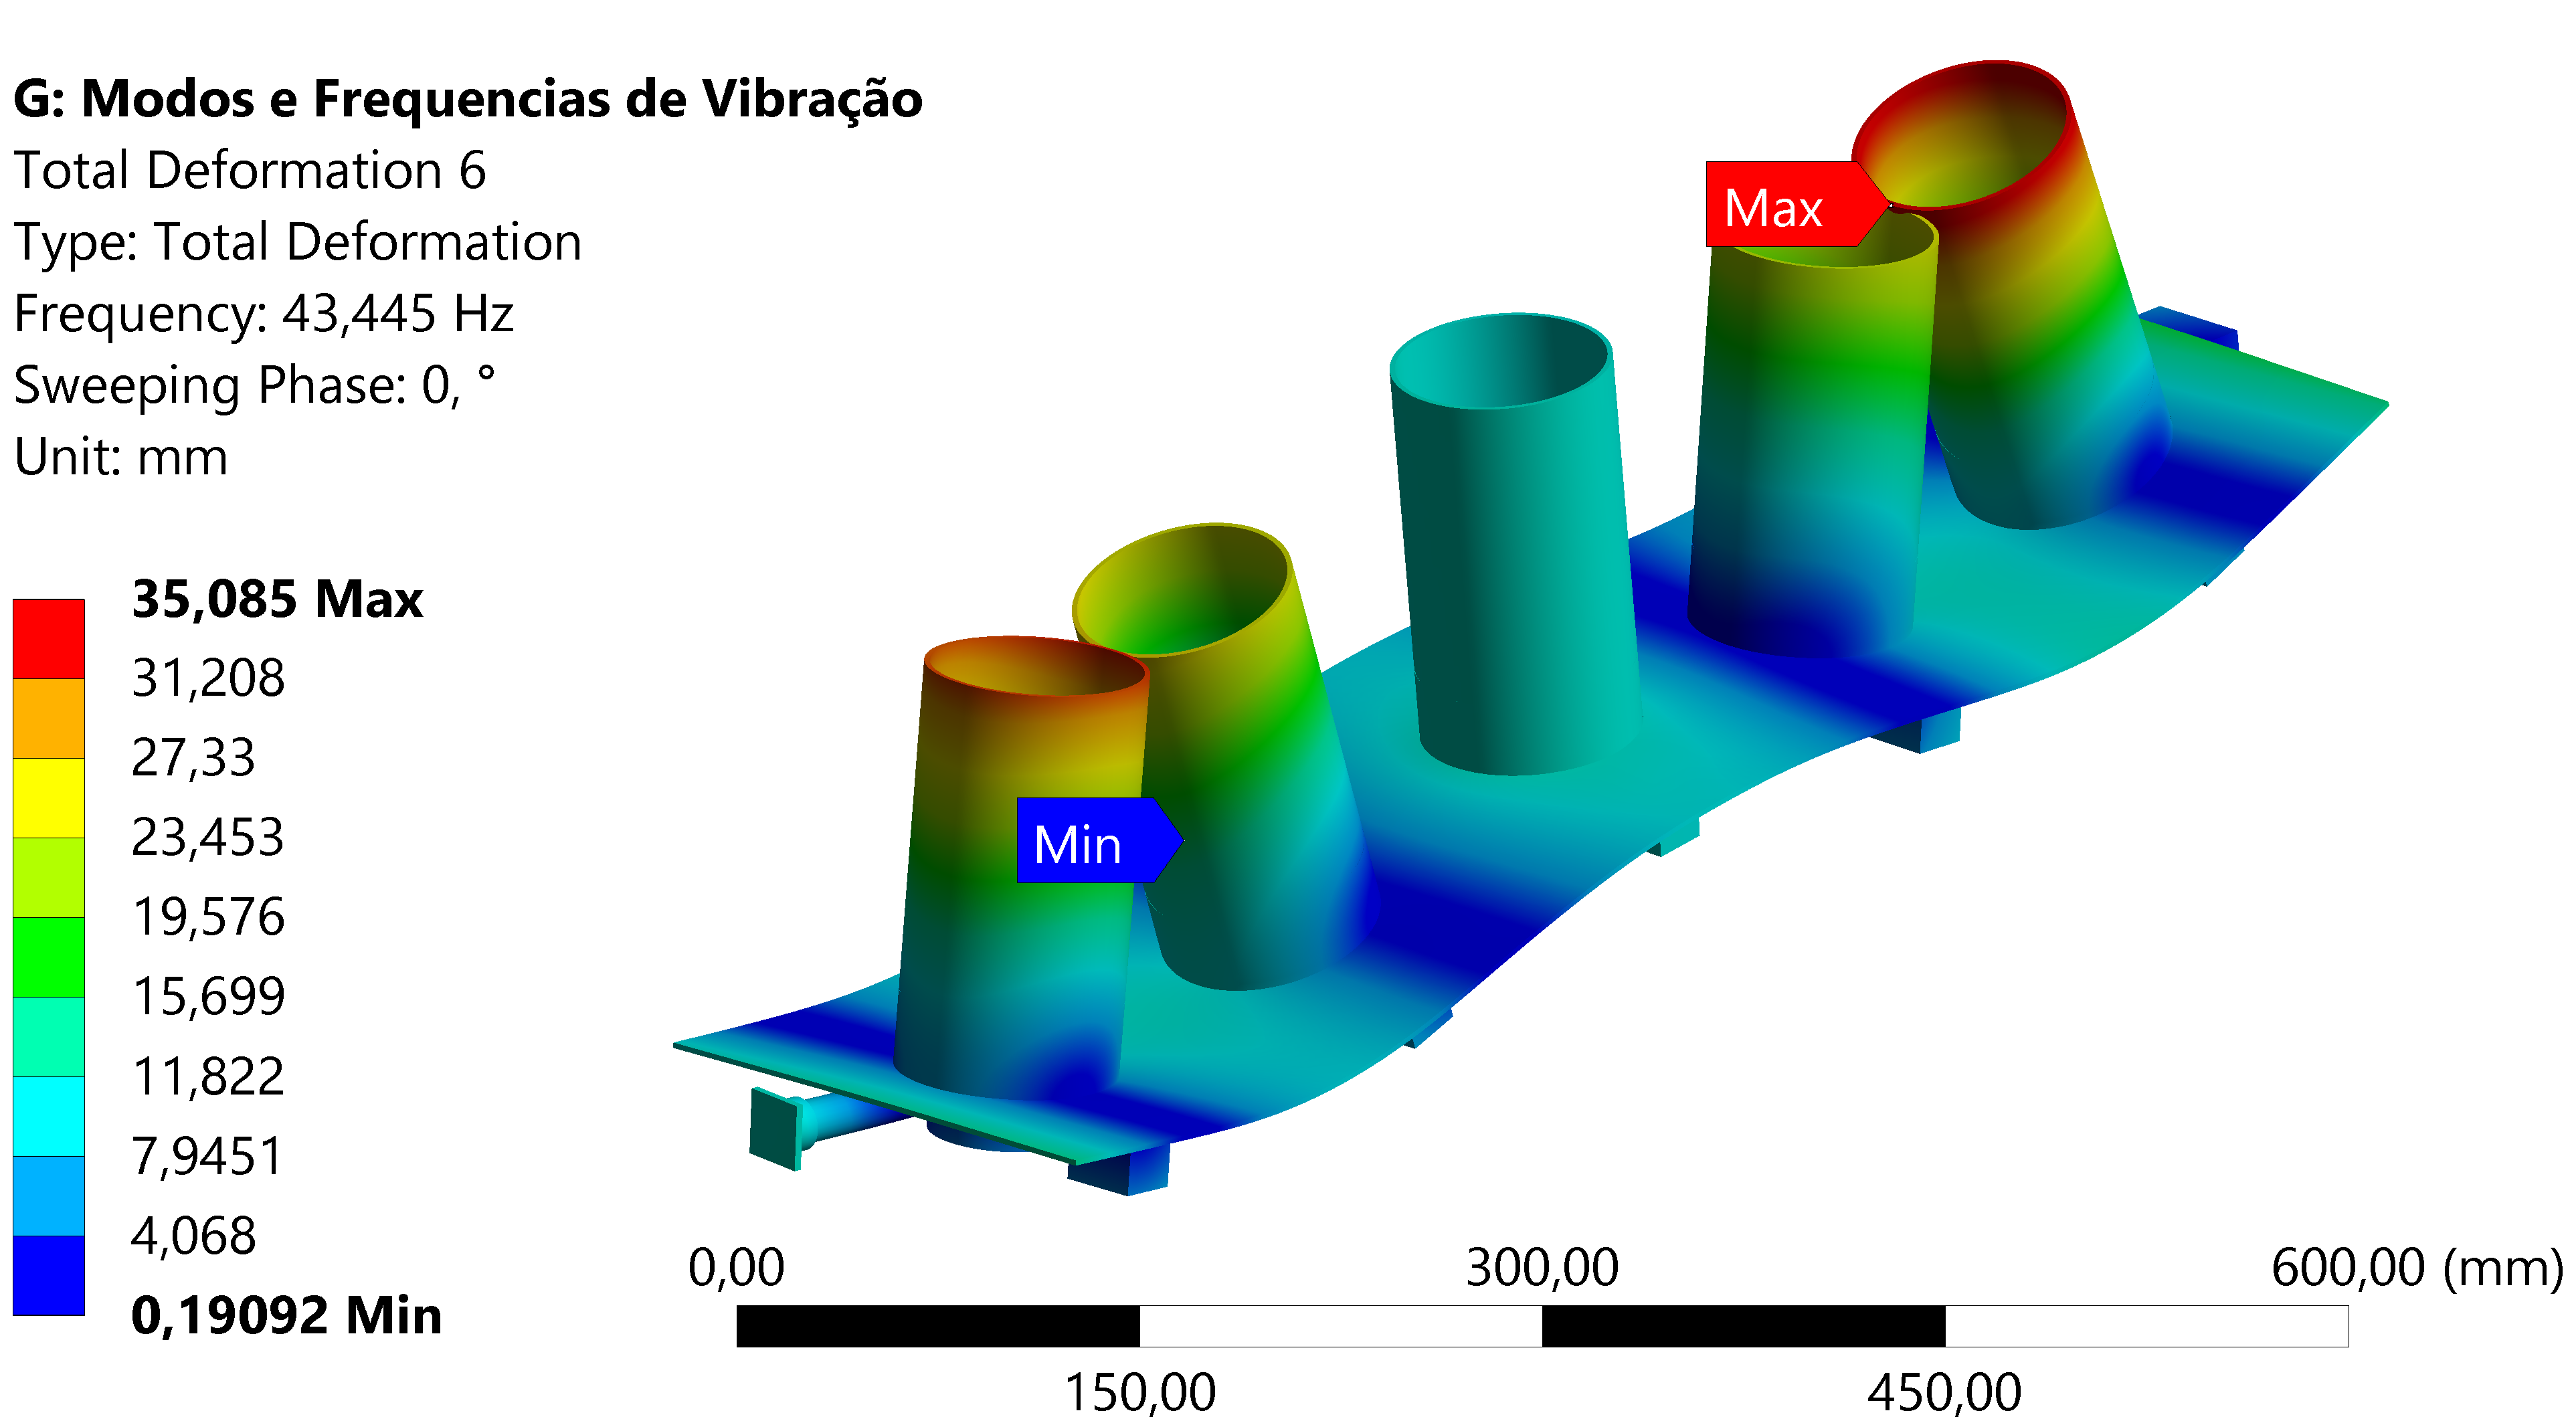
\includegraphics[width=.5\linewidth]{figuras/estrutura/Imagens PC3/Vibrações/modo 6.png}}\par 
\caption{Representação das formas modais 5 e 6}
\label{fig:modos56}
\end{figure}

\begin{figure}[ht]
\centering
\subfloat[Modo 7]{\label{fig:modo7}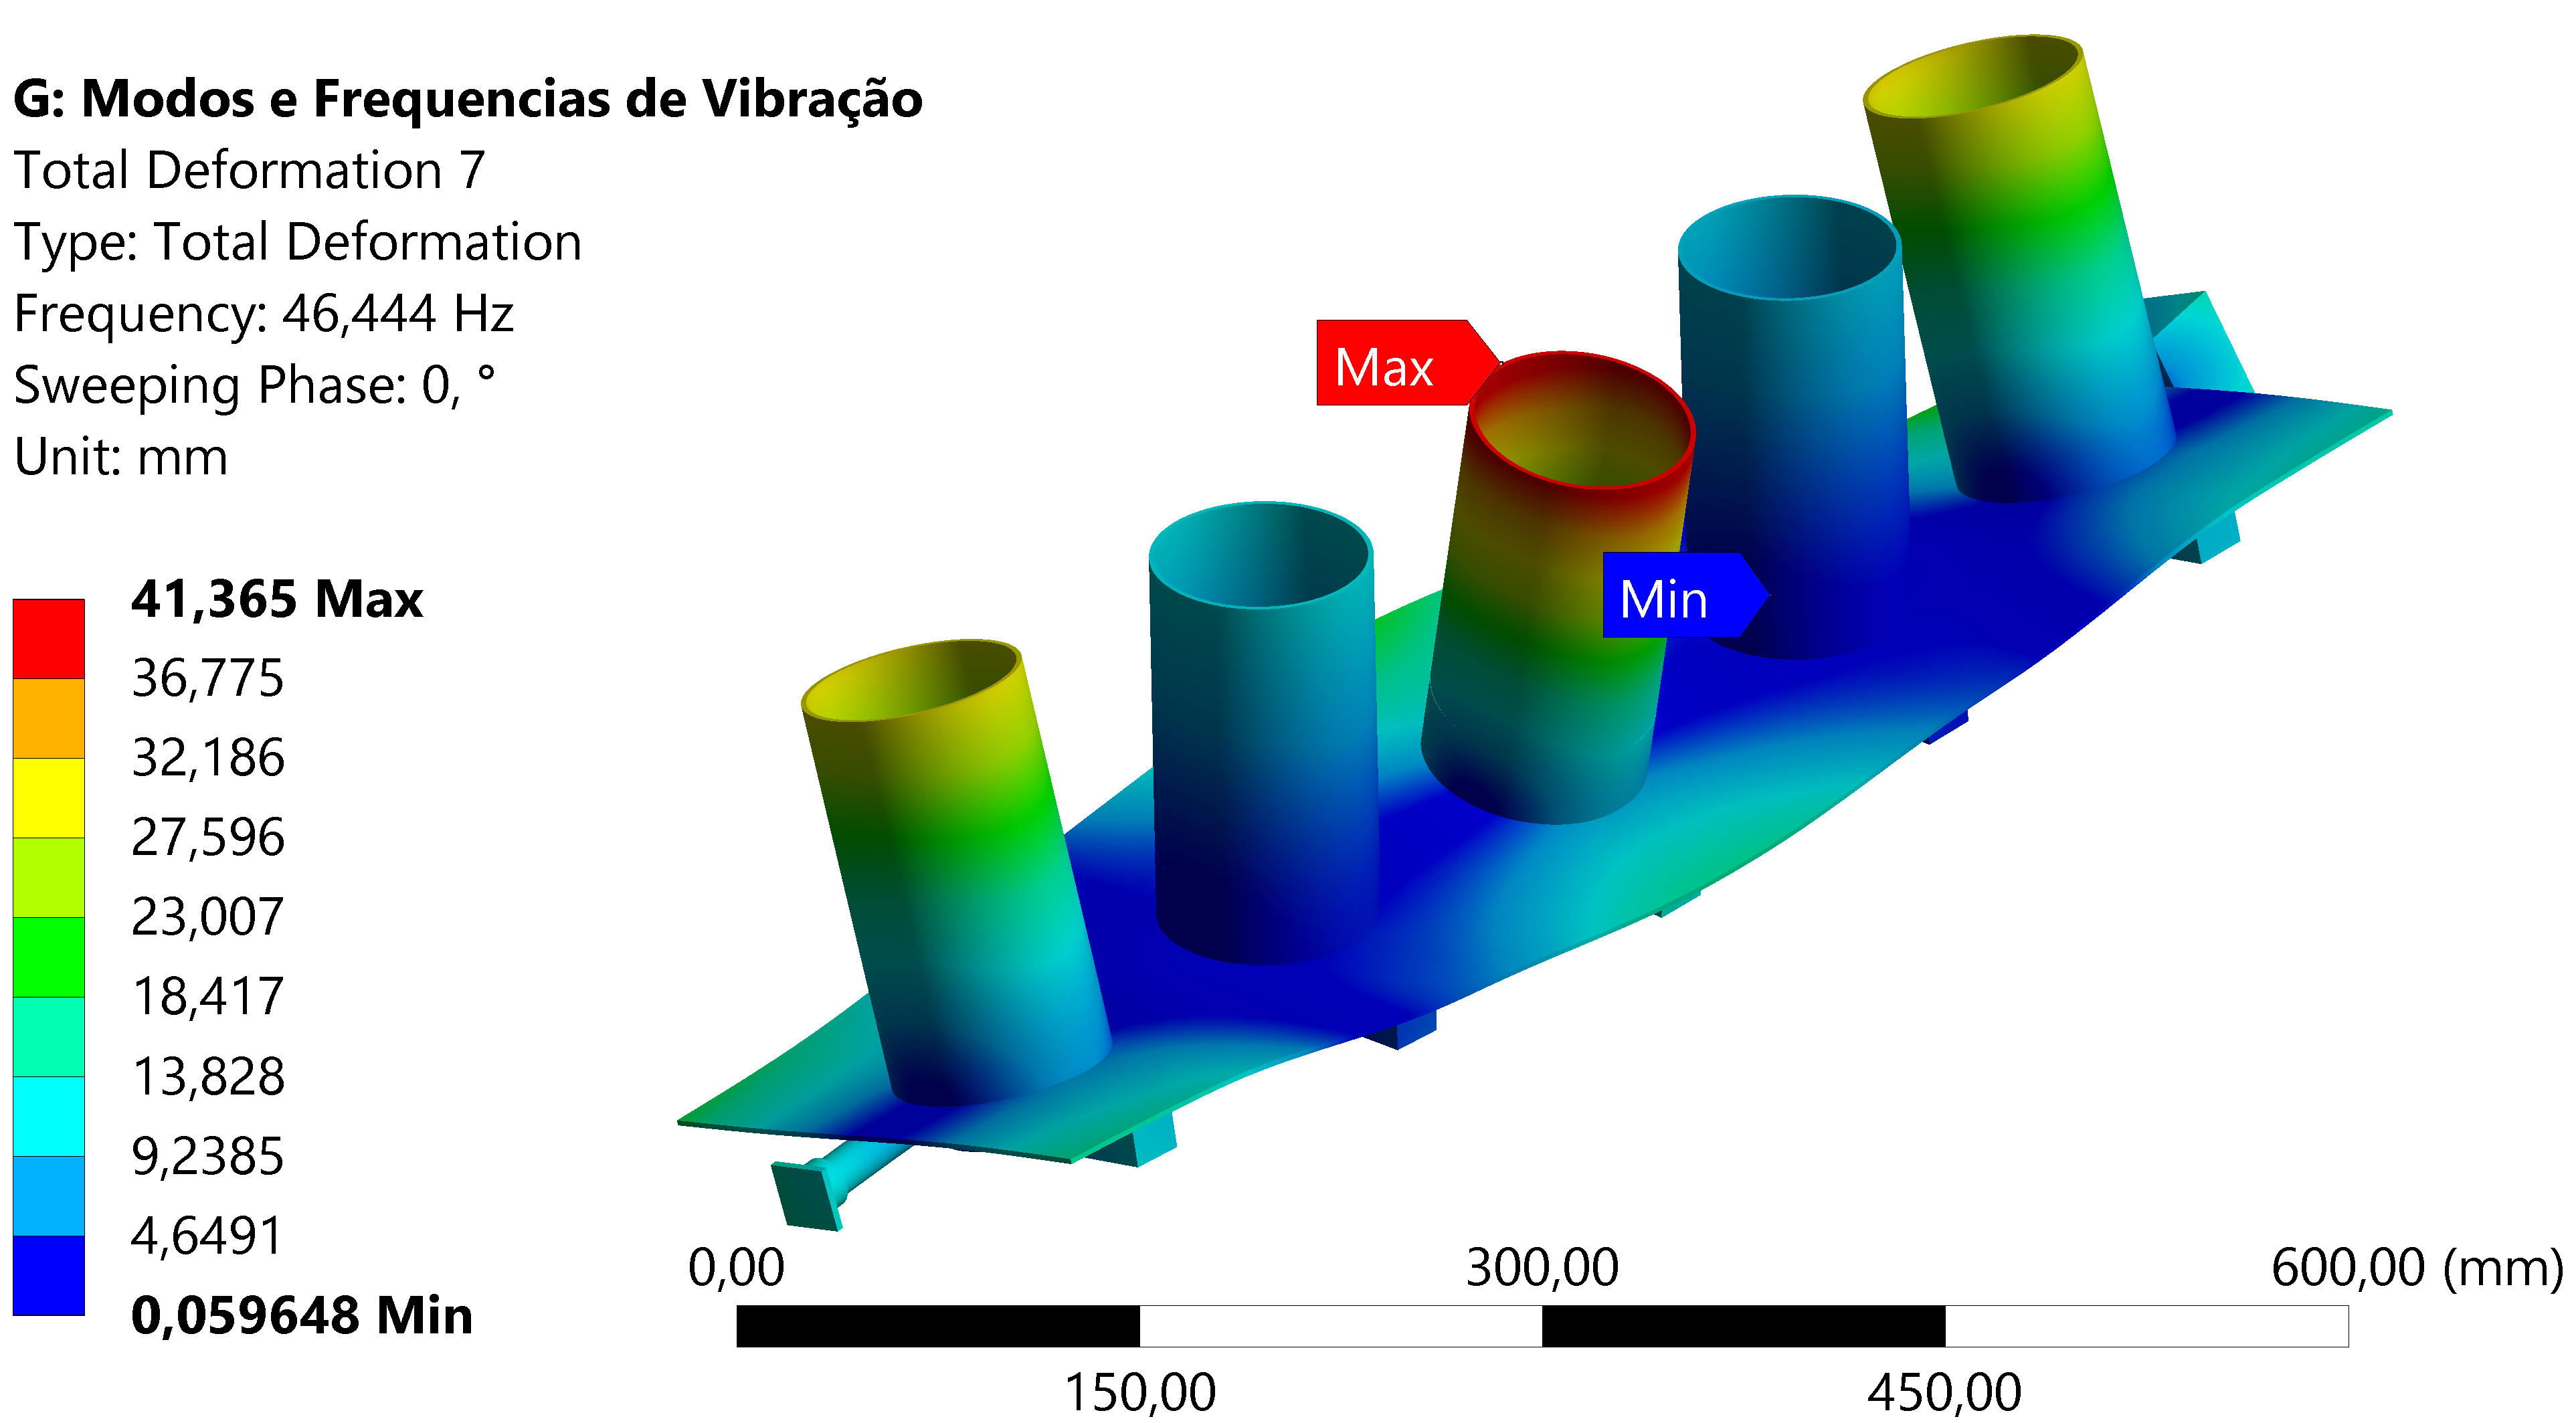
\includegraphics[width=.5\linewidth]{figuras/estrutura/Imagens PC3/Vibrações/modo 7.png}}\hfill
\subfloat[Modo 8]{\label{fig:modo8}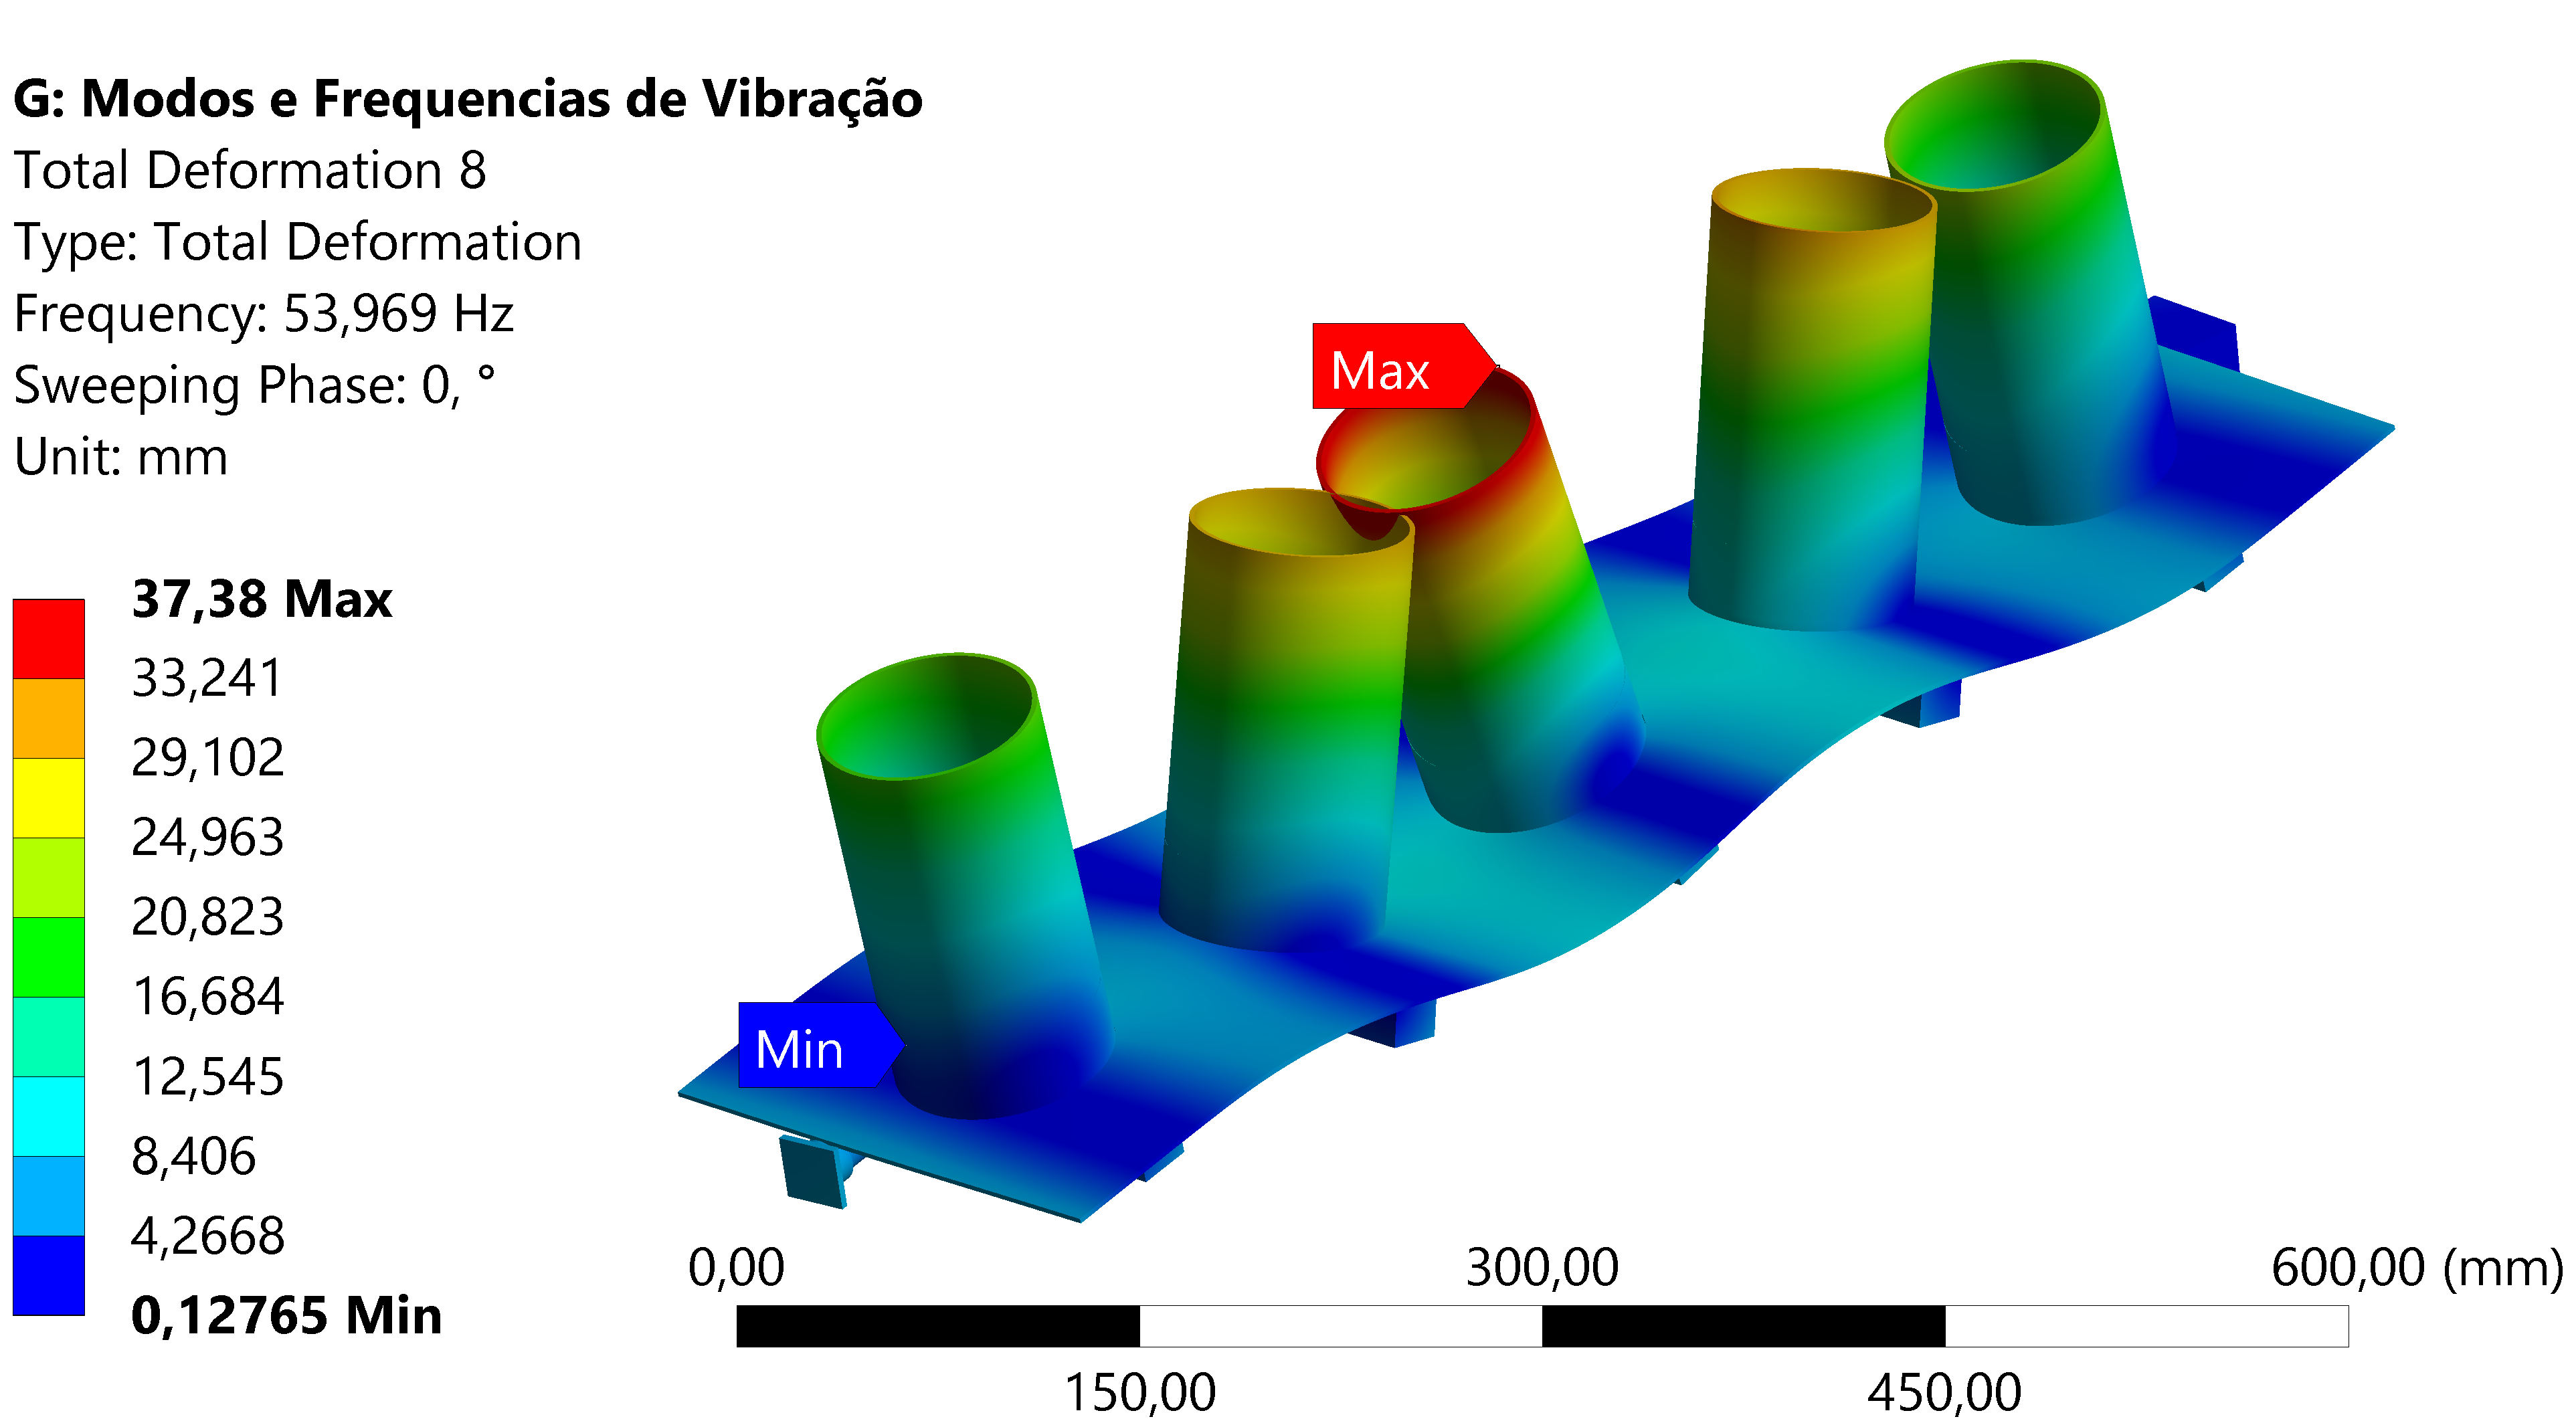
\includegraphics[width=.5\linewidth]{figuras/estrutura/Imagens PC3/Vibrações/modo 8.png}}\par 
\caption{Representação das formas modais 7 e 8}
\label{fig:modos78}
\end{figure}

\begin{figure}[ht]
\centering
\subfloat[Modo 9]{\label{fig:modo9}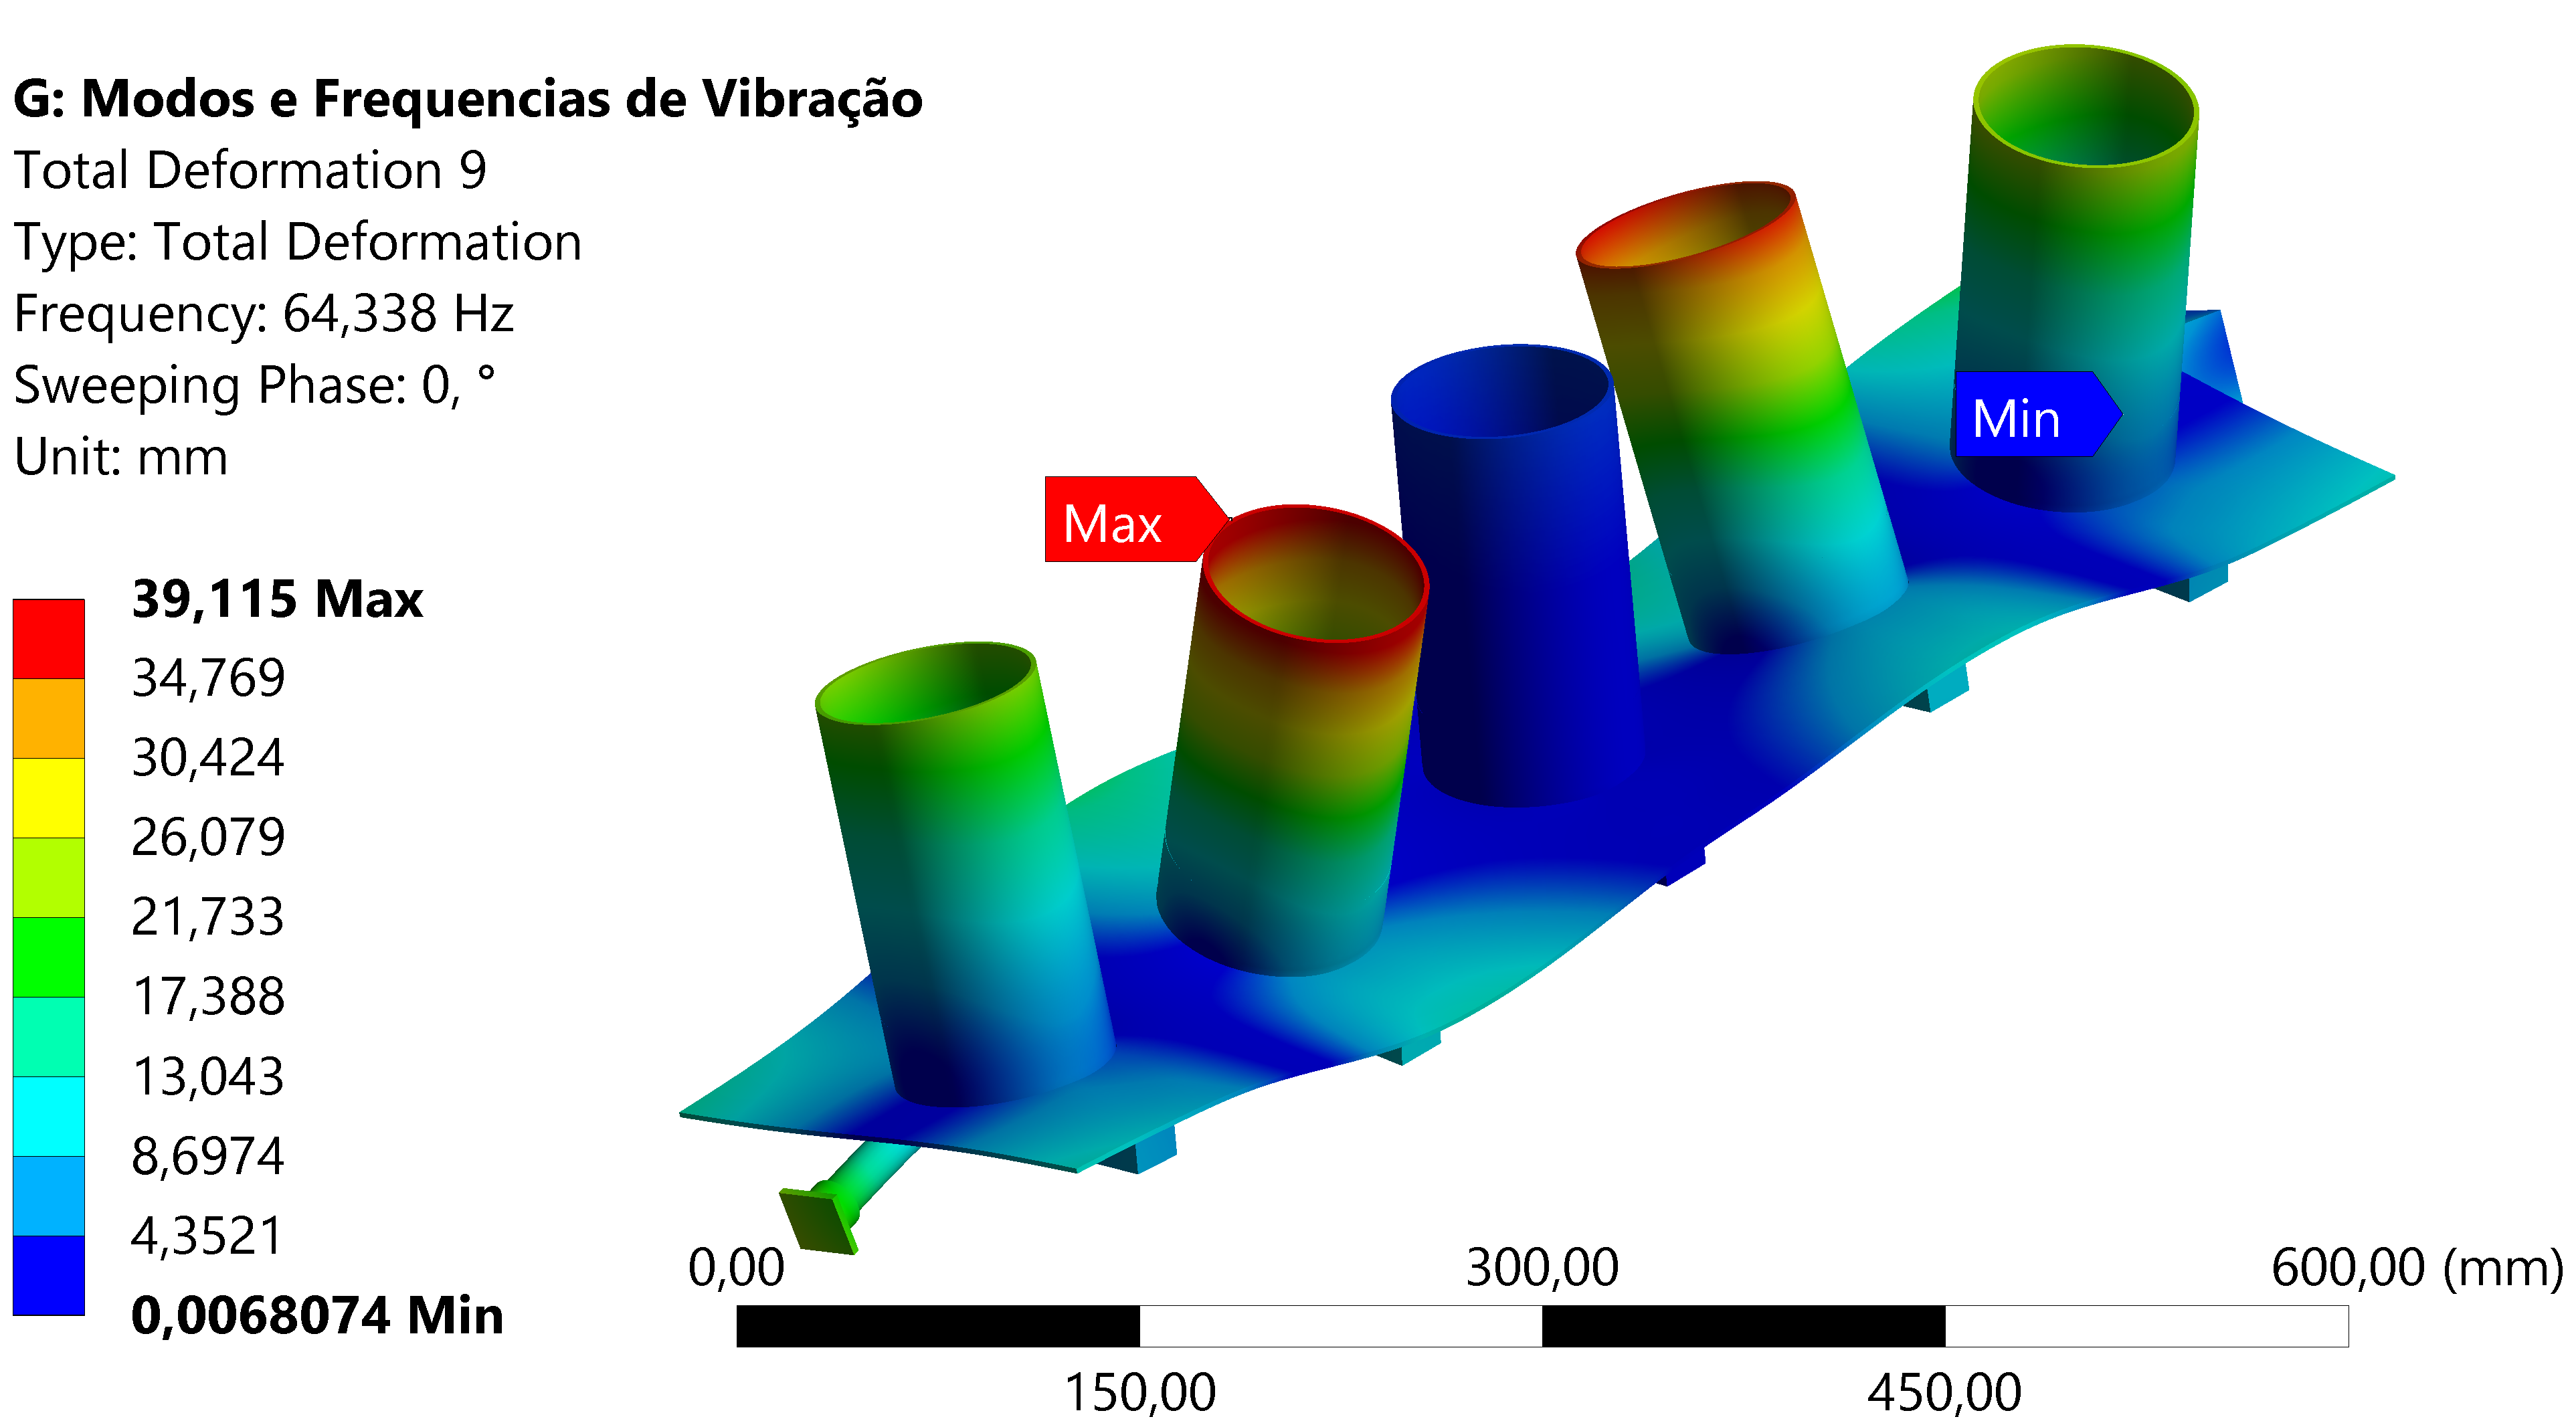
\includegraphics[width=.5\linewidth]{figuras/estrutura/Imagens PC3/Vibrações/modo 9.png}}\hfill
\subfloat[Modo 10]{\label{fig:modo10}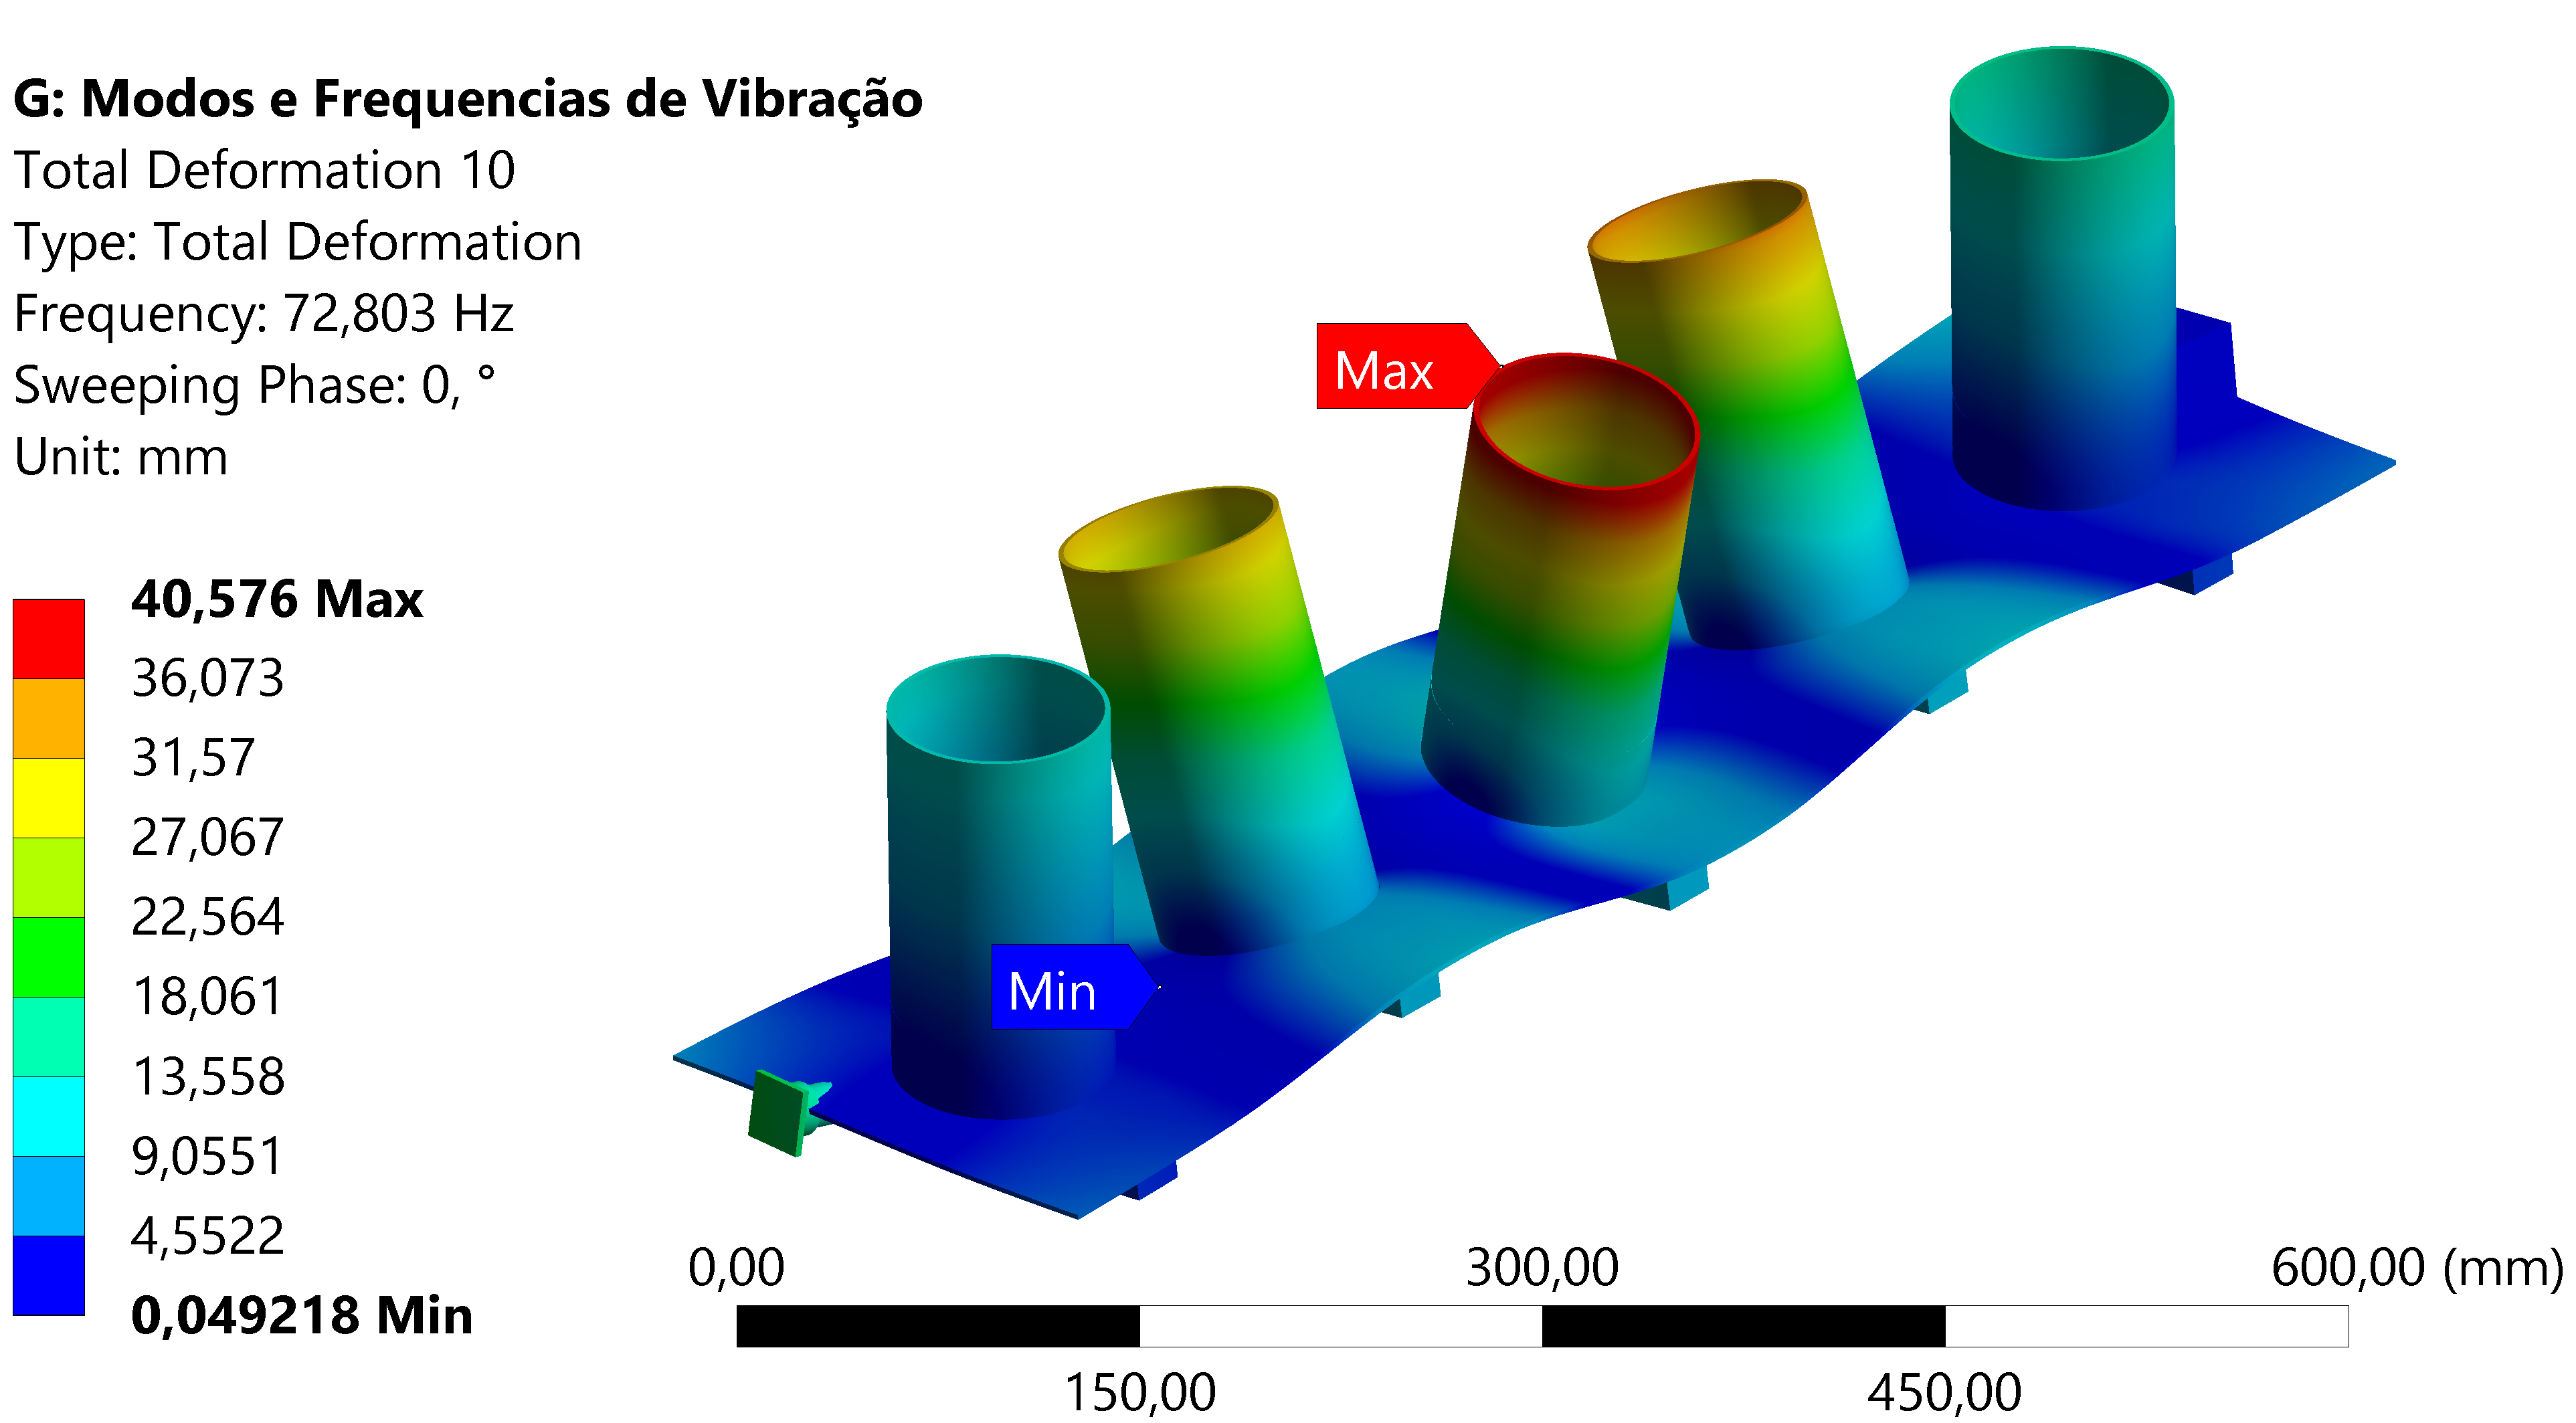
\includegraphics[width=.5\linewidth]{figuras/estrutura/Imagens PC3/Vibrações/modo 10.png}}\par 
\caption{Representação das formas modais 9 e 10}
\label{fig:modos910}
\end{figure}

Pela análise dos resultados, observa-se nós (efeitos nulos de deformação ou aproximadamente nulos) em cima dos contêiners 2 e 5 para o modo 1 (Fig. \ref{fig:modo1}), alto deslocamento da parte traseira do motor para o modo 2 (Fig. \ref{fig:modo2}), efeito similar no modo 3 (Fig. \ref{fig:modo3}) e efeito simétrico de deformação nos modos 4 e 5 (Fig. \ref{fig:modo4} e \ref{fig:modo5}). Para os modos 6 e 8 (Fig. \ref{fig:modo6} e \ref{fig:modo8}) verificam-se novamente os nós oscilando entre os compartimentos. Finalmente, os modos 7, 9 e 10 (Fig. \ref{fig:modo7}, \ref{fig:modo9} e \ref{fig:modo10}, respectivamente) apresentam efeitos de deformação nula em formato de cruz, passando por dentro dos contêiners de uma extremidade à outra no eixo do fuso e de uma lateral à outra nos centros dos objetos.  Um resumo das frequências naturais é disponibilizado na Tab. \ref{tab:modos}. 
\begin{table}[ht]
    \centering
    \footnotesize
    \caption{Tabela de Frequências Naturais do sistema}
    \label{tab:modos}
    \begin{adjustbox}{max width = \textwidth}
        \begin{tabular}{|c|c|}
            \hline
            \rowcolor[HTML]{A8DADC}
            \textbf{Modo} & \textbf{Frequência [Hz]}  \\ \hline
            1 & 11,4 \\ 
            \hline
            2 & 20,1 \\
            \hline
            3 & 21,6 \\
            \hline
            4 & 28,9 \\
            \hline
            5 & 30,9 \\
            \hline
            6 & 43,4 \\
            \hline
            7 & 46,4 \\
            \hline
            8 & 54,0 \\
            \hline
            9 & 64,3 \\
            \hline
            10 & 72,8 \\
            \hline
        \end{tabular}
    \end{adjustbox}
\end{table}

Como efeito conclusivo ao estudo, ressalta-se que a primeira frequência natural presente no modelo modal está contida na faixa de 11 Hz, enquanto a faixa de excitação do motor, conforme já citada no dimensionamento do fuso (seção \ref{section:dimensionamento_F_E}), opera em 2,6 Hz (158 rpm) e, portanto, há uma ampla margem de oscilação para a operação do componente, sem preocupações com as junções ou a estrutura como um todo no aspecto de vibrações. 

\subsection{Análise Térmica} \label{section:AnaliseTermica}
%\subparagraph*{$\bullet$ Análise térmica} \hfill


Com as dimensões e materiais da estrutura definidos, podemos embasar um estudo acerca da transferência de calor dentro do dispositivo. O dimensionamento do problema térmico compreende garantir que a temperatura interna dos contêineres seja limitado superior e inferiormente por um valor que não comprometa as propriedades dos medicamentos. 

Como já exposto anteriormente, nos objetivos específicos (veja \ref{section:Obj_esp}), as restrições seriam equivalentes a temperaturas acima de 15 $^{\circ}$C e abaixo de 30 $^{\circ}$C. Ressalta-se que a validação proposta aqui dita um comportamento do sistema afim garantir que o fluxo de calor advindo dos componentes eletrônicos não resulte em uma elevada temperatura interna através de arranjos da geometria interna.

  

Para o caso da solução proposta, compreende-se o subsistema simplificado já apresentado, com o incremento de um volume de controle e duas peças geradoras de potência (Atuador e \textit{Raspberry}). A Fig. \ref{fig:subgrupo_termico} exibe a configuração adotada para o problema térmico.

\begin{figure}[ht]
        \centering
        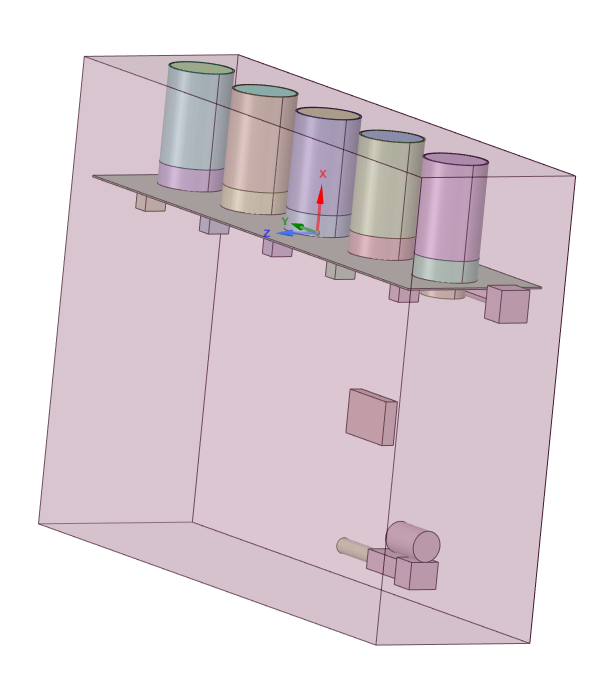
\includegraphics[width=.4\textwidth]{figuras/estrutura/Modelagem térmica/Geometria simplificada.png}
        \caption{Geometria simplificada para estudo da transferência de calor}
        \label{fig:subgrupo_termico}
    \end{figure}

Fisicamente falando, temos um problema que é caracterizado por uma convecção natural com o ar como fluido, fontes de calor oriundas apenas de componentes eletrônicos, atuando com mecanismos de transmissão por condução do núcleo até a superfície e difusão com ar \cite{transcal}. Como meios de condução, além dos componentes eletrônicos, teremos as partes físicas do subgrupo. As propriedades térmicas consideradas na simulação para cada material estão apresentadas na Tab. \ref{tab:Propriedadestermicas}.

\begin{table}[H]
    \centering
    \caption{}
    \label{tab:Propriedadestermicas}
    \begin{adjustbox}{max width = \textwidth}
        \begin{tabular}{|C{3.5cm}|C{4cm}|C{3.5cm}|C{4cm}|}
            \hline
            \rowcolor[HTML]{A8DADC}
            \textbf{Material} & \textbf{Coeficiente de Expansão Térmica \qquad  (K$^{-1}$)} & \textbf{Calor específico (J$\cdot$ kg$^{-1}\cdot$ K$^{-1}$)} & \textbf{Condutividade térmica isotrópica (J$\cdot$m$^{-1}\cdot$ s$^{-1}\cdot$ K$^{-1}$)} \\ \hline
              \textit{Nylon} 6.6 & 1,28 $\cdot10^{-4} $ & 1520 & 0,24 \\ \hline
              Polipropileno & 1,03 $\cdot10^{-4} $ & 1680 & 0,21 \\ \hline
              Aço Estrutural  & 1,20 $\cdot10^{-5} $ & 434 & 60,50 \\ \hline
              Aço Inox 304  & 1,70 $\cdot10^{-5} $ & 510 & 15 \\ \hline
              Aço SAE 1020  & 1,19 $\cdot10^{-5}$ & 486 & 51,90 \\ \hline
              Cobre  & 1,80 $\cdot10^{-5} $ & 385 & 401 \\\hline
             
        \end{tabular}
    \end{adjustbox}
\end{table}


As primeiras aproximações feitas no problema incluem a análise do problema de calor que inclui um subgrupo composto por:
\begin{itemize}
    \item Cinco cilindros com parede finita, as dimensões são idênticas as paredes cilíndricas nos contêineres (veja a cotagem \ref{fig:cilindro}) e do mesmo material (Aço Inoxidável 304).
    \item Cinco cilindros sólidos substituindo as partes da rampa, plataforma de seleção, engrenagens e compartimentos inferiores, sendo do material Polipropileno e mesmas dimensões da base do contêiner (veja cotagem \ref{fig:conteiner}). 
    \item Mesa de sustentação dos cilindros, com dimensões idênticas as do design inicial (veja cotagem \ref{fig:base_subgrupo}) e do mesmo material (Aço carbono SAE 1020).
    \item Cinco caixas menores em formato quadricular, representando os motores solenoides e acoplados à base de sustentação do cilindros, o material seria genérico (Aço estrutural).
    \item Uma caixa maior em formato quadricular, representando o motor de passo do subsistema, esta um pouco à frente dos cilindros, material genérico (Aço estrutural).
    \item Estrutura cilíndrica de mesmo comprimento e diâmetro do fuso do design inicial (veja cotagem \ref{fig:engrenagem_fundo}) e do mesmo material (\textit{Nylon} 6.6).
    \item Uma caixa em formato retangular, representando a \textit{Raspberry} em modelo de temperatura uniforme, presente abaixo do subgrupo de contêineres, material (liga de cobre presente no ANSYS).
    \item Uma versão simplificada do atuador linear presente desde a escolha preliminar do projeto, material genérico (Aço estrutural).
    \item Caixa de ar formulando o volume de controle da simulação de comprimento suficientemente grande para cobrir toda a estrutura a ser simulada (800x600x230 mm$^3$)
\end{itemize}

Para cargo de informação ao leitor, a Tab. \ref{fig:energia_carga} , presente na solução energética, descreve a carga global e potências geradas pelo componentes elétricos e eletrônicos escolhidos para o sistema, e com o auxílio da análise feita pelo projeto da fonte (veja tópico \ref{section:energia_fonte}), observamos que o cenário 4 representa o estado da máquina que consumiria a maior quantidade de energia e os componentes responsáveis pelo consumo. Com ambas as informações, conseguimos caracterizar a análise transiente da temperatura global do sistema, onde iremos preliminarmente agrupar os componentes em funcionamento no cenário ao longo do tempo. Para critério de simplificação, adotará-se um modelo onde:
\begin{itemize}
    \item As potências dos sensores fotoelétricos, por proximidade física, serão posicionadas nas faces de baixo dos solenoides;
    \item As potências da \textit{Raspberry}, dos microcontroladores, do visor e dos \textit{drivers} L298 e do motor de passo serão inseridas como fontes de calor internas à \textit{Raspberry};
    \item As potências do atuador linear, da câmera e do sensor RFID, por proximidade física, serão acopladas no interior da fonte de calor do Atuador. 
    \item O motor de passo terá uma potência interna gerada em conjunto com a potência do sensor de temperatura.
\end{itemize}

A próxima etapa descreve o funcionamento temporal do sistema, e caracteriza-se com funcionamento permanente dos sensores, câmeras, microcontroladores e visor (100\% da potência a todo instante), \textit{Raspberry} com operação de 50 a 100\% da potência máxima presente na tabela supracitada, motor de passo ativo durante a rotação do fuso do subgrupo, além do funcionamento do atuador linear e \textit{drivers} por 5 segundos com escala linear de aumento e declínio de potência. A Tab. \ref{tab:estruturas_termica} ilustra o funcionamento do sistema simplificado:

\begin{table}[H]
    \centering
    \caption{Comportamento temporal das potências do Sistema}
    \label{tab:estruturas_termica}
    \begin{adjustbox}{max width = \textwidth}
        \begin{tabular}{|C{2cm}|C{3cm}|C{3cm}|C{3cm}|C{3cm}|C{3cm}|C{4cm}}
            \hline
            \rowcolor[HTML]{A8DADC}
            \textbf{Tempo (s)}&\textbf{Raspberry (W)} & \textbf{Atuador Linear (W) } & \textbf{Motor de Passo (W)} & \textbf{Solenoides (W)} & \textbf{Total (W)} \\ \hline
            0 & 8,00 & 0,75 & 0 & 2,50 & 11,25
            \\ \hline
              5 & 45,90	 & 24,75  & 4,80 & 2,50 & 78,00
             \\ \hline 
             10 &  12,15 & 0,75 & 4,80 & 2,50 & 20,20
             \\ \hline
             30 & 12,15	 & 0,75  & 4,80 & 2,50 & 20,20
             \\ \hline
              32 & 15,90 & 0,75 & 2,90 & 2,50 & 22,10
             \\ \hline
              37 & 41,10 & 24,75 & 0 & 2,50 & 68,40
             \\ \hline
              42 & 12,15 & 0,75 & 0 & 2,50 & 15,40
             \\ \hline
              62 & 12,15 & 0,75 & 0 & 2,50 & 15,40
             \\ \hline
              64 & 15,90 & 0,75 & 0 & 2,50 & 19,20
             \\ \hline
              69 & 41,10 & 24,75 & 0 & 2,50 & 68,40
             \\ \hline
              74 & 12,15 & 0,75 & 0 & 2,50 & 15,40
             \\ \hline
               94 & 12,15 & 0,75 & 0 & 2,50 & 15,40
             \\ \hline
                96 & 15,90 & 0,75 & 0 & 2,50 & 19,20
             \\ \hline
              101 & 41,10 & 24,75 & 0 & 2,50 & 68,40
             \\ \hline
              106 & 12,15 & 0,75 & 0 & 2,50 & 15,40
             \\ \hline
             126 & 12,15 & 0,75 & 0 & 2,50 & 15,40
             \\ \hline
            128 & 15,90 & 0,75 & 0 & 2,50 & 19,20
             \\ \hline
            133 & 35,10 & 24,75 & 0 & 2,50 & 68,40
             \\ \hline
             138 & 12,50 & 0,75 & 0 & 2,50 & 15,40
             \\ \hline
        158  & 12,50 & 0,75 & 0 & 2,50 & 15,40
             \\ \hline
             163  & 8,40 & 0,8 & 0 & 2,50 & 11,70
             \\ \hline
        7200  & 8,40 & 0,8 & 0 & 2,50 & 11,70
             \\ \hline
        
        \end{tabular}
    \end{adjustbox}
\end{table}

Para as condições de contorno do problema, foram estabelecidas curvas de potência com os dados inscritos na Tab. \ref{tab:estruturas_termica} fornecidas através das fontes internas para o caso do atuador, da \textit{Raspberry} e do motor de passo, e da representação de fontes de calor nas faces dos solenoides para representar os sensores fotoelétricos. 

Foi escolhido a temperatura ambiente local como 22 $^{\circ}$C, meio de convecção como ar com respectivo coeficiente de convecção igual a $5$ {W}/m$^{2}$. As paredes superiores e laterais teriam temperatura inicial de 22 $^{\circ}$C e tempo de simulação com duração de 2 horas (7200 segundos), sendo os 2 minutos e 43 segundos iniciais a etapa do funcionamento de um ciclo completo da máquina.

Dos resultados obtidos das Fig. \ref{fig:calor_normal} e \ref{fig:calor_volume}, observamos um comportamento praticamente idêntico a condição inicial, com variação da temperatura local próxima as fontes de calor mais acentuada porém com baixa intensidade, sendo levemente dissipada ao longo das duas horas. 

\begin{figure}[ht]
        \centering
        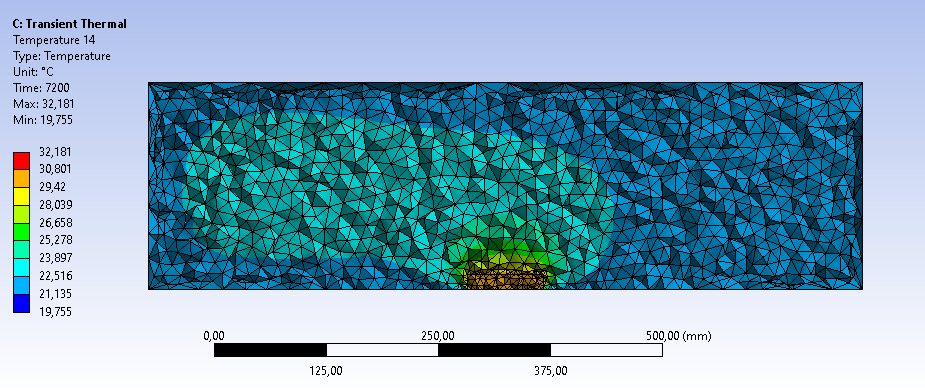
\includegraphics[width=0.85\textwidth]{figuras/estrutura/Modelagem térmica/horizontal.png}
        \caption{Trasferência de calor normal ao volume de controle}
        \label{fig:calor_normal}
    \end{figure}
    
    \begin{figure}[H]
        \centering
        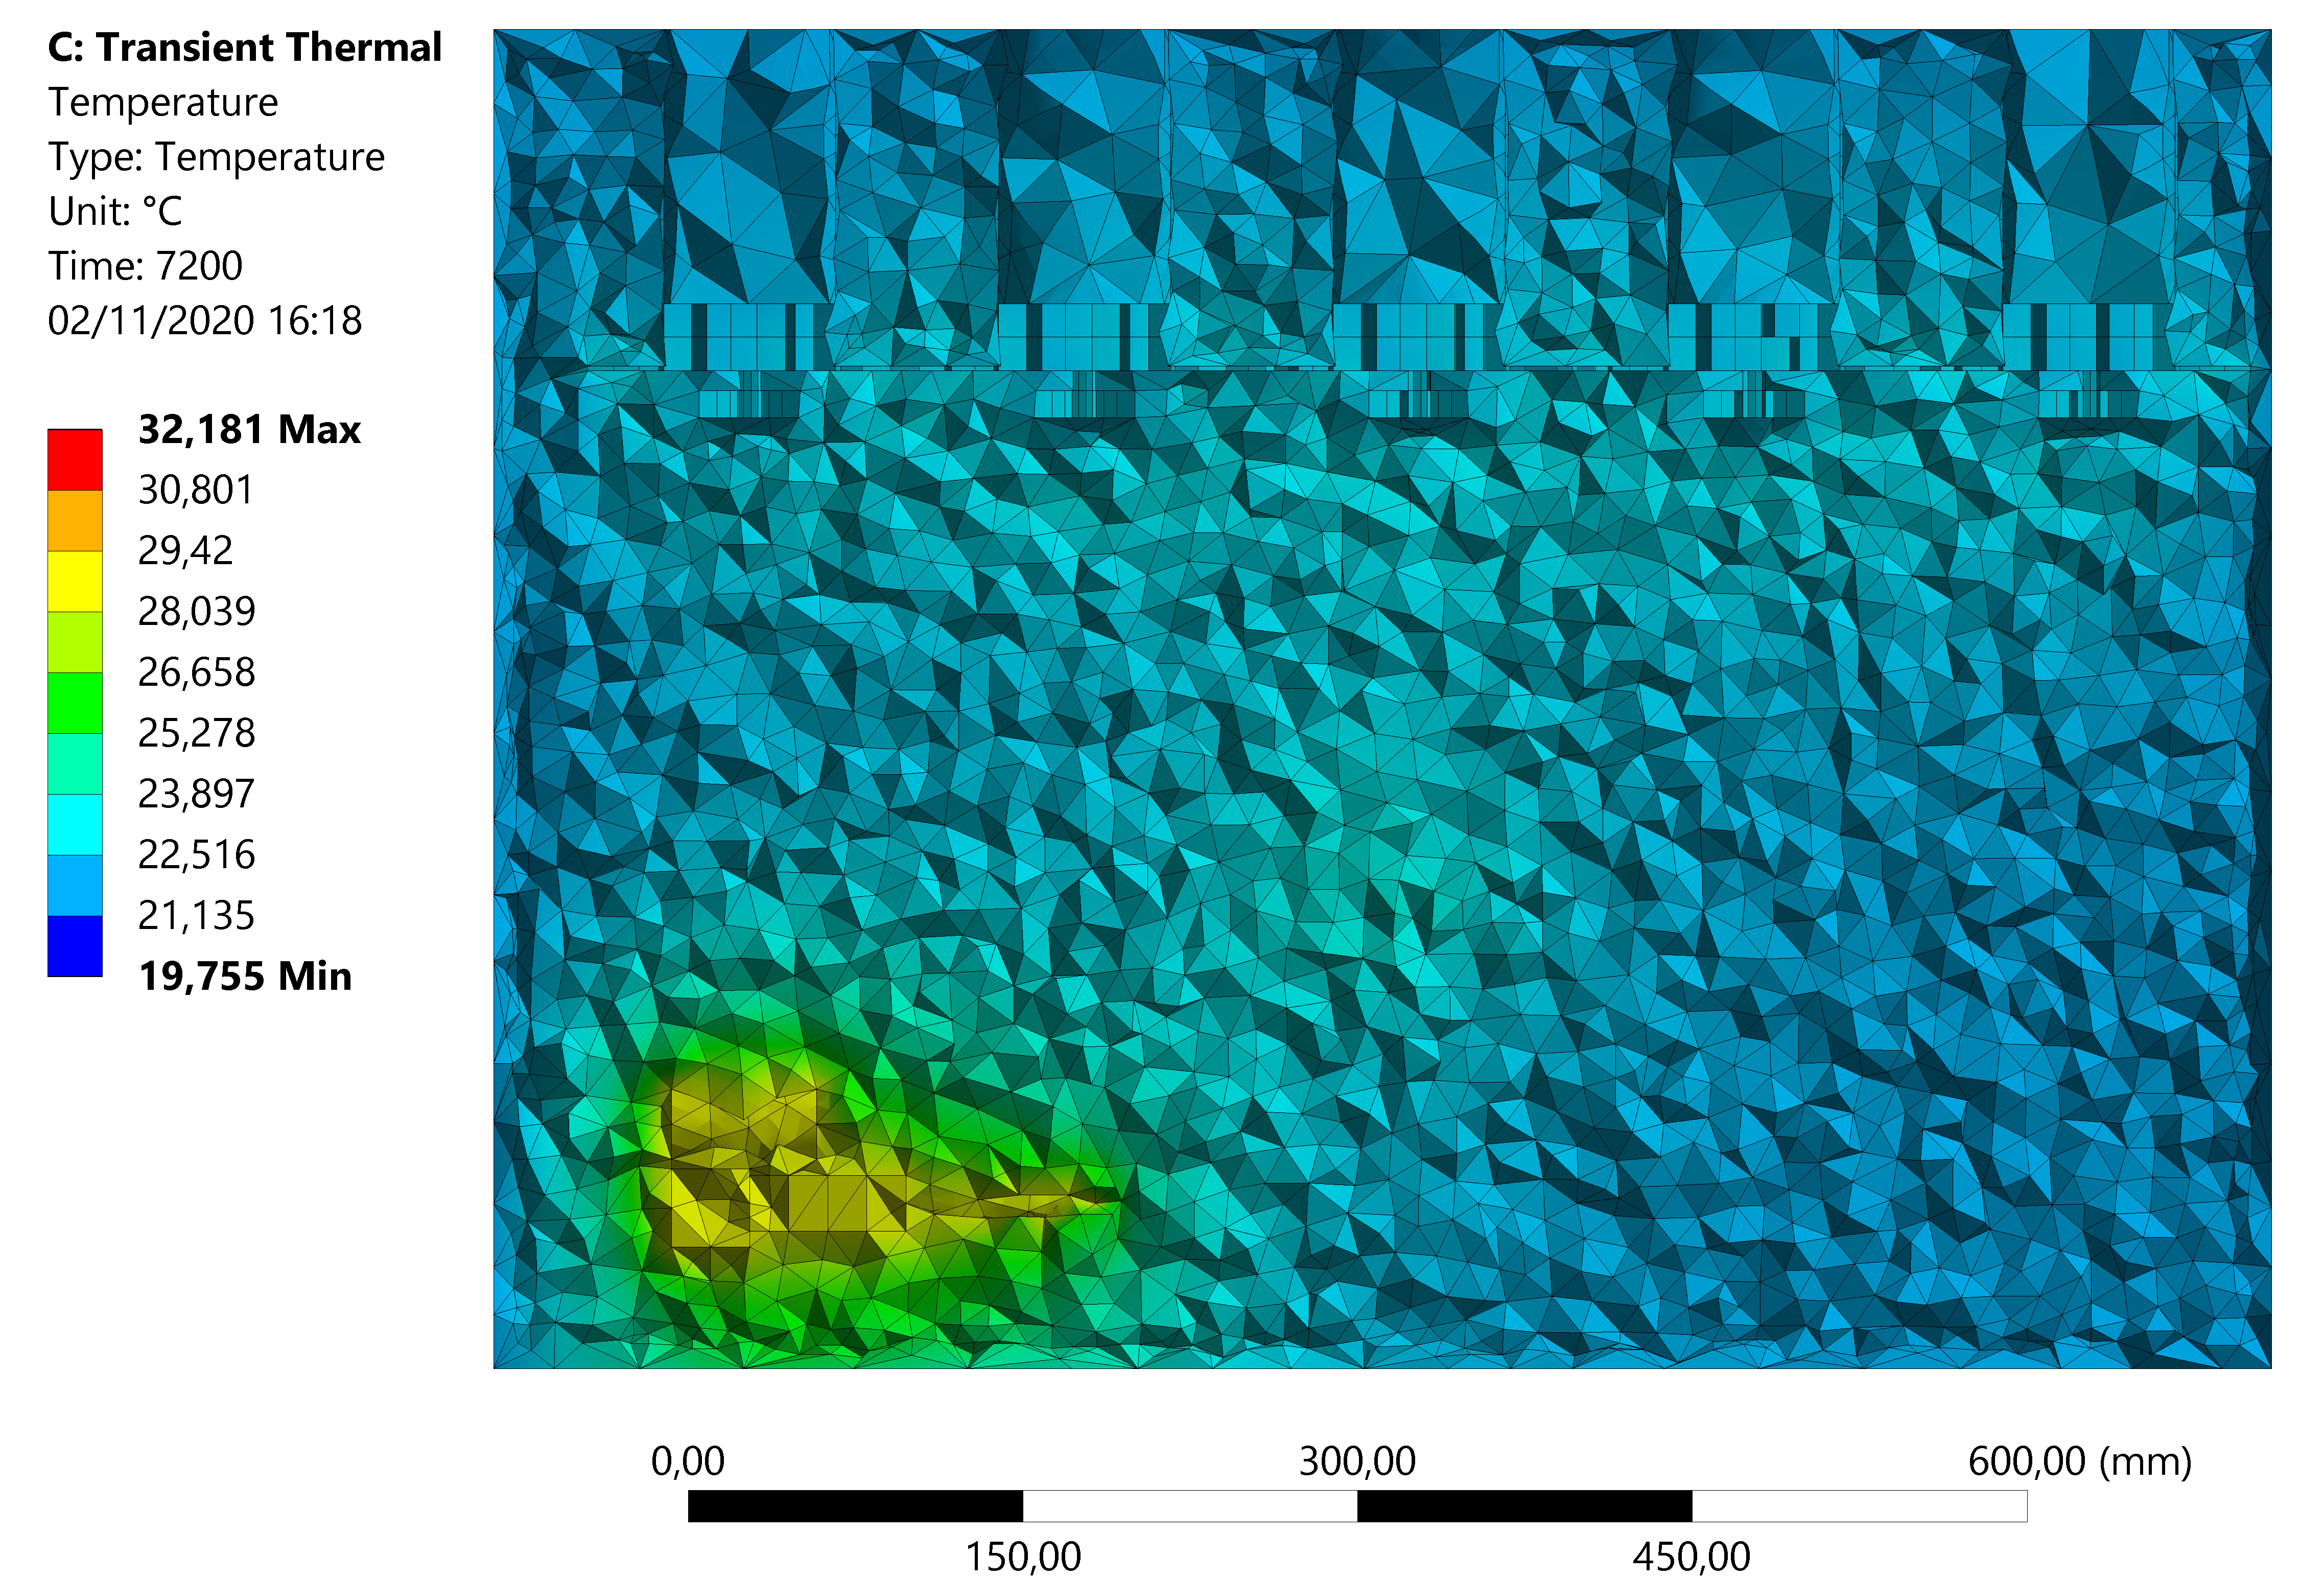
\includegraphics[width=0.8\textwidth]{{figuras/estrutura/Modelagem térmica/volume.png}}
        \caption{Transferência de calor dentro do volume de controle}
        \label{fig:calor_volume}
    \end{figure}
 %   
%  \begin{figure}[ht]
%        \centering
%        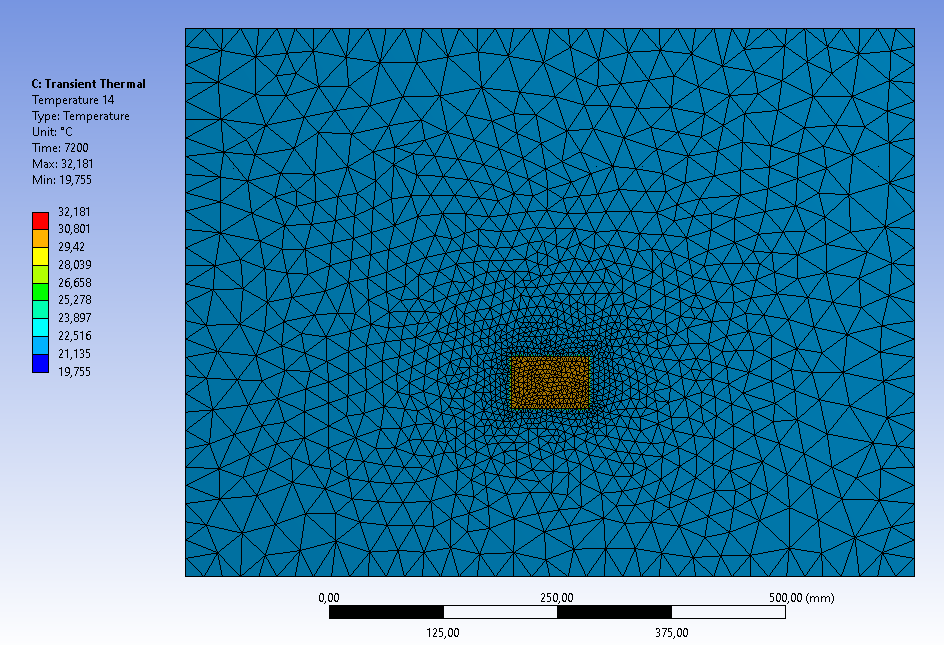
\includegraphics[width=.8\textwidth]{{figuras/estrutura/Modelagem térmica/placa.png}}
 %       \caption{Transferência de calor no plano da placa do circuito}
 %       \label{fig:calor_plano}
  %  \end{figure}

Com relação às temperaturas máxima e mínima, iremos fazer o uso do gráfico de convergência da temperatura máxima, apresentado na Fig. \ref{fig:temp_max}.

 \begin{figure}[H]
        \centering
        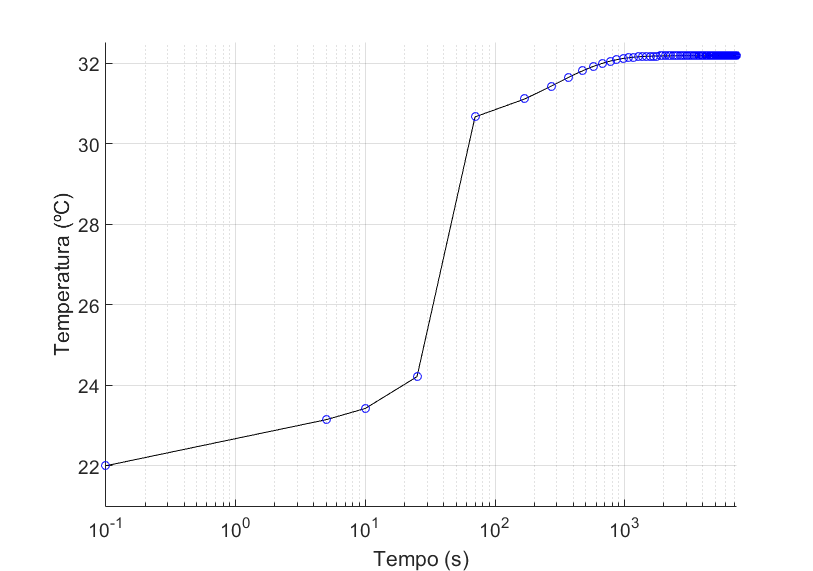
\includegraphics[width=.8\textwidth]{{figuras/estrutura/Modelagem térmica/grafico.png}}
        \caption{Temperatura máxima alcançada ao longo do tempo}
        \label{fig:temp_max}
    \end{figure}

Observamos que o modelo atinge para o valor limite de temperatura de 32,2 $^{\circ}$C em torno de 23 minutos dentro da placa retangular durante o processo de resfriamento do sistema pelo ambiente. Logo após o período de alta taxa de transferência de calor, a temperatura global sobe um pouco, e a temperatura da fonte principal de calor \textit{(Raspberry)} começa a baixar sua temperatura e normaliza em torno de 30,8 $^{\circ}$C. Apesar da alta temperatura, por conta das propriedades isolantes do meio (ar), as temperaturas elevadas são isoladas e levemente são dissipadas sem uma propagação intensa da onda de calor. Por conta disso, as temperaturas dos contêineres puderam ser controladas sem a necessidade de um mecanismo ativo de controle de temperatura.

Com relação à temperatura mínima, observamos uma discordância em razão da aproximação numérica, onde por conta do passo finito dos nós da malha, obtivemos resultados de absorção de calor nas proximidades da placa emissora. As consequências do resultado não têm impacto na análise, visto que são pontos com temperaturas dentro da faixa do modelo, e não são suficientemente altas para causar uma divergência do resultado final da simulação. Resultados podem ser conferidos na Fig. \ref{fig:erros}.

 \begin{figure}[ht]
        \centering
        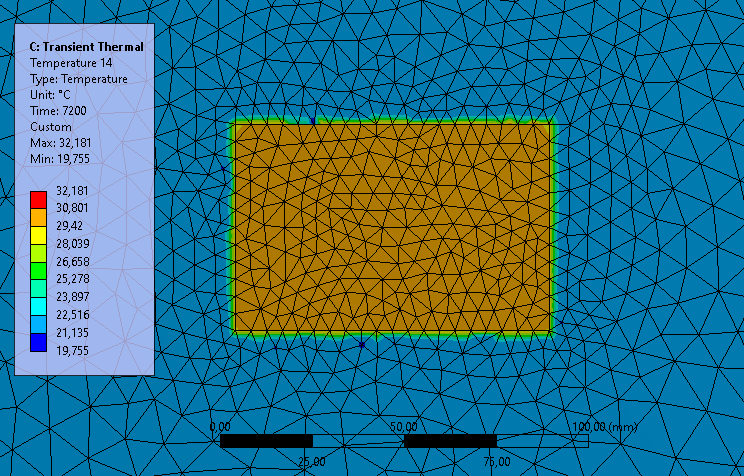
\includegraphics[width=.8\textwidth]{{figuras/estrutura/Modelagem térmica/erro.png}}
        \caption{Erros gerados pelas dimensões finitas do método computacional}
        \label{fig:erros}
    \end{figure}
    
Com o auxílio da simulação, pudemos verificar um aumento mínimo de temperatura na região de interesse, ou seja, na zona dos contêineres, correspondente a 1,5 $^{\circ}$C de acréscimo temperatura global, e consequentemente, aprova a construção de um dispositivo para começar o planejamento de utilização do sistema para armazenagem de medicamentos em casos gerais de temperatura ambiente, com faixa equivalente de 13,5 $^{\circ}$C a 28,5 $^{\circ}$C, possivelmente expansíveis por fontes externas de refrigeração/aquecimento, mas vale destacar a necessidade de isolamento adequado do sistema à fontes de calor exteriores (como o Sol, por exemplo).

Como efeito conclusivo, também foi possível aferir que há uma margem significativamente
alta para se realizar uma redistribuição espacial dos componentes fornecedores de calor, desde que não sejam posicionados suficientemente
próximos dos contêiners, de um modo a qual poderiam alterar significativamente a temperatura local dos comprimidos, como
pudemos observar com os resultados obtidos para as vizinhanças das fontes de calor.
